% Research note: closing edge loops at quantization time (the applied paper;
% the theory of obstructions is in the companion note, docs/research/turns-of-a-t-mesh).
% Build: `make paper NOTE=closing-loops` from the root of the repository, which
% first writes version.tex (the commit described, \enginecommit); without it,
% or by hand: pdflatex paper && bibtex paper && pdflatex paper && pdflatex paper
\documentclass[11pt,a4paper]{article}

\usepackage[T1]{fontenc}
\usepackage[utf8]{inputenc}
\usepackage{lmodern}
\usepackage[margin=2.5cm]{geometry}
\usepackage{amsmath,amssymb,amsthm}
\usepackage{booktabs}
\usepackage{array}
\usepackage{graphicx}
\usepackage{tikz}
\usetikzlibrary{arrows.meta,decorations.pathreplacing}
\usepackage[numbers,sort&compress]{natbib}
\usepackage[hidelinks]{hyperref}
\setlength{\emergencystretch}{2em}
% Room for the full-width figures of Section 6 at the top of a page.
\renewcommand{\topfraction}{0.9}
\renewcommand{\dbltopfraction}{0.9}
\renewcommand{\floatpagefraction}{0.8}
\renewcommand{\dblfloatpagefraction}{0.8}

\newtheorem{definition}{Definition}
\newtheorem{proposition}{Proposition}

\newcommand{\Z}{\mathbb{Z}}
\newcommand{\shift}{s}

% The commit of the engine described, written by `make paper` into
% version.tex (ignored by git).
\IfFileExists{version.tex}{\input{version.tex}}{}
\providecommand{\enginecommit}{unknown}

% Levels of evidence: each statement and table is framed with a tag naming
% what checks it (Lean, the engine's data, a measure, the proof on paper, a
% citation), read from the README of ../turns-of-a-t-mesh/lean, as in the companion
% paper. evidence.py, in that folder, checks that every statement has a level
% and that every Lean name cited is declared there. \def\plain{} before % Research note: closing edge loops at quantization time (the applied paper;
% the theory of obstructions is in the companion note, docs/research/turns-of-a-t-mesh).
% Build: `make paper NOTE=closing-loops` from the root of the repository, which
% first writes version.tex (the commit described, \enginecommit); without it,
% or by hand: pdflatex paper && bibtex paper && pdflatex paper && pdflatex paper
\documentclass[11pt,a4paper]{article}

\usepackage[T1]{fontenc}
\usepackage[utf8]{inputenc}
\usepackage{lmodern}
\usepackage[margin=2.5cm]{geometry}
\usepackage{amsmath,amssymb,amsthm}
\usepackage{booktabs}
\usepackage{array}
\usepackage{graphicx}
\usepackage{tikz}
\usetikzlibrary{arrows.meta,decorations.pathreplacing}
\usepackage[numbers,sort&compress]{natbib}
\usepackage[hidelinks]{hyperref}
\setlength{\emergencystretch}{2em}
% Room for the full-width figures of Section 6 at the top of a page.
\renewcommand{\topfraction}{0.9}
\renewcommand{\dbltopfraction}{0.9}
\renewcommand{\floatpagefraction}{0.8}
\renewcommand{\dblfloatpagefraction}{0.8}

\newtheorem{definition}{Definition}
\newtheorem{proposition}{Proposition}

\newcommand{\Z}{\mathbb{Z}}
\newcommand{\shift}{s}

% The commit of the engine described, written by `make paper` into
% version.tex (ignored by git).
\IfFileExists{version.tex}{\input{version.tex}}{}
\providecommand{\enginecommit}{unknown}

% Levels of evidence: each statement and table is framed with a tag naming
% what checks it (Lean, the engine's data, a measure, the proof on paper, a
% citation), read from the README of ../turns-of-a-t-mesh/lean, as in the companion
% paper. evidence.py, in that folder, checks that every statement has a level
% and that every Lean name cited is declared there. \def\plain{} before % Research note: closing edge loops at quantization time (the applied paper;
% the theory of obstructions is in the companion note, docs/research/turns-of-a-t-mesh).
% Build: `make paper NOTE=closing-loops` from the root of the repository, which
% first writes version.tex (the commit described, \enginecommit); without it,
% or by hand: pdflatex paper && bibtex paper && pdflatex paper && pdflatex paper
\documentclass[11pt,a4paper]{article}

\usepackage[T1]{fontenc}
\usepackage[utf8]{inputenc}
\usepackage{lmodern}
\usepackage[margin=2.5cm]{geometry}
\usepackage{amsmath,amssymb,amsthm}
\usepackage{booktabs}
\usepackage{array}
\usepackage{graphicx}
\usepackage{tikz}
\usetikzlibrary{arrows.meta,decorations.pathreplacing}
\usepackage[numbers,sort&compress]{natbib}
\usepackage[hidelinks]{hyperref}
\setlength{\emergencystretch}{2em}
% Room for the full-width figures of Section 6 at the top of a page.
\renewcommand{\topfraction}{0.9}
\renewcommand{\dbltopfraction}{0.9}
\renewcommand{\floatpagefraction}{0.8}
\renewcommand{\dblfloatpagefraction}{0.8}

\newtheorem{definition}{Definition}
\newtheorem{proposition}{Proposition}

\newcommand{\Z}{\mathbb{Z}}
\newcommand{\shift}{s}

% The commit of the engine described, written by `make paper` into
% version.tex (ignored by git).
\IfFileExists{version.tex}{\input{version.tex}}{}
\providecommand{\enginecommit}{unknown}

% Levels of evidence: each statement and table is framed with a tag naming
% what checks it (Lean, the engine's data, a measure, the proof on paper, a
% citation), read from the README of ../turns-of-a-t-mesh/lean, as in the companion
% paper. evidence.py, in that folder, checks that every statement has a level
% and that every Lean name cited is declared there. \def\plain{} before % Research note: closing edge loops at quantization time (the applied paper;
% the theory of obstructions is in the companion note, docs/research/turns-of-a-t-mesh).
% Build: `make paper NOTE=closing-loops` from the root of the repository, which
% first writes version.tex (the commit described, \enginecommit); without it,
% or by hand: pdflatex paper && bibtex paper && pdflatex paper && pdflatex paper
\documentclass[11pt,a4paper]{article}

\usepackage[T1]{fontenc}
\usepackage[utf8]{inputenc}
\usepackage{lmodern}
\usepackage[margin=2.5cm]{geometry}
\usepackage{amsmath,amssymb,amsthm}
\usepackage{booktabs}
\usepackage{array}
\usepackage{graphicx}
\usepackage{tikz}
\usetikzlibrary{arrows.meta,decorations.pathreplacing}
\usepackage[numbers,sort&compress]{natbib}
\usepackage[hidelinks]{hyperref}
\setlength{\emergencystretch}{2em}
% Room for the full-width figures of Section 6 at the top of a page.
\renewcommand{\topfraction}{0.9}
\renewcommand{\dbltopfraction}{0.9}
\renewcommand{\floatpagefraction}{0.8}
\renewcommand{\dblfloatpagefraction}{0.8}

\newtheorem{definition}{Definition}
\newtheorem{proposition}{Proposition}

\newcommand{\Z}{\mathbb{Z}}
\newcommand{\shift}{s}

% The commit of the engine described, written by `make paper` into
% version.tex (ignored by git).
\IfFileExists{version.tex}{\input{version.tex}}{}
\providecommand{\enginecommit}{unknown}

% Levels of evidence: each statement and table is framed with a tag naming
% what checks it (Lean, the engine's data, a measure, the proof on paper, a
% citation), read from the README of ../turns-of-a-t-mesh/lean, as in the companion
% paper. evidence.py, in that folder, checks that every statement has a level
% and that every Lean name cited is declared there. \def\plain{} before \input{paper} gives the paper
% without them, for a venue that wants it plain.
\newcommand{\lean}[1]{\texttt{\detokenize{#1}}}
\ifdefined\plain
\newenvironment{evidence}[3][]{}{}
\else
\usepackage[most]{tcolorbox}
\newcommand{\evlevel}[2]{\expandafter\newcommand\csname ev-name-#1\endcsname{#2}}
\evlevel{lean}{Lean, complete}
\evlevel{core}{Lean, algebraic core}
\evlevel{data}{Checked on the engine's data}
\evlevel{measured}{Measured}
\evlevel{prose}{Proof on paper only}
\evlevel{tested}{Conjecture, checked by computer}
\evlevel{cited}{Standard, cited}
\evlevel{open}{Open, no claim}
\newcommand{\evname}[1]{\csname ev-name-#1\endcsname}
\tcbset{evstyle-lean/.style={}, evstyle-core/.style={}, evstyle-data/.style={},
  evstyle-measured/.style={}, evstyle-tested/.style={}, evstyle-prose/.style={},
  evstyle-cited/.style={},
  evstyle-open/.style={frame hidden, borderline={0.4pt}{0pt}{black!45, dashed}}}
\newtcolorbox{evidence}[3][]{breakable, enhanced, colback=white,
  colframe=black!45, boxrule=0.4pt, arc=0pt, left=4pt, right=4pt, top=2pt,
  bottom=2pt, before skip=6pt, after skip=6pt, evstyle-#2,
  title={\footnotesize\textsc{\evname{#2}}\if\relax\detokenize{#3}\relax\else
    \quad #3\fi},
  coltitle=black, colbacktitle=white, titlerule=0.4pt, toptitle=1pt,
  bottomtitle=1pt, #1}
\fi

\title{Closing Edge Loops at Quantization Time:\\
Helix Constraints for T-Mesh Quantization\\[0.5em]
\large Research note --- draft, not peer reviewed}
\author{Marc Gardent%
\thanks{This note is distributed under the Creative Commons Attribution
4.0 International licence (CC BY 4.0). The code of openclare is under the
GPL-3.0-or-later of the repository. The note describes the engine at commit
\texttt{\enginecommit} of \url{https://github.com/marcgardent/openclare}.
A French translation is in \texttt{paper.fr.pdf}, beside this note.}\\
\normalsize Independent researcher\\
\normalsize ORCID: \href{https://orcid.org/0009-0000-6466-3098}{0009-0000-6466-3098}\\
\normalsize Contact: through the repository,
\url{https://github.com/marcgardent/openclare}}
\date{October 2026}

\begin{document}
\maketitle

\begin{abstract}
Automatic quad remeshing often produces edge loops that wind round a part of
the shape as helices instead of closing into rings. Bommes et
al.~\cite{bommes2011structure} remove such \emph{q-helices} from a finished
mesh; we prevent them where the integer structure of the mesh is decided, in
the quantization of a T-mesh. A straight walk across the patches of a T-mesh
that returns to its first side, a \emph{turn}, has a \emph{shift} that is an
integer linear form in the arc lengths; at whole lengths it is how far the
strip of quads following the turn comes back beside itself, and every strip
of the mesh is such a walk. We add the constraints that close turns to a
minimum-deviation quantizer~\cite{heistermann2023bimdf}, through a
least-change projection, repair walks and rounds of constraint generation on
the strips of the mesh, and keep the candidate with the fewest spiral edges,
counted by a test that tells helices from closed, open and border loops. Over
twelve models at three budgets near 3{,}000 quads, the engine leaves 4.92\%
of the edges on spiral loops (19.8\% without closing); on the seven models
that two other open-source remeshers also mesh validly, 2.2\% against 38.8\% % NIGHT4
and 21.7\%; on a human body, 1.5\%, against 2.5\% for the hand-made mesh.
An exact analysis of the closing system of that body shows that the conflict between closing
turns and keeping singularities apart is real but local, that the heuristic
rather than the constraints leaves most turns shifted, and that closing more
turns does not by itself make fewer spirals: the strips move with the
lengths, and the choice of the turns to close decides.
\end{abstract}

\section{Introduction}

In our experience, element shape and alignment are rarely what limits
field-aligned quad remeshing today (see the
surveys~\cite{bommes2013survey,campen2017survey}). What remains is structure:
the way edge loops run across the surface. Artists expect a loop round an
arm, a leg or a neck to be a ring. Automatic methods often produce a helix
instead: the loop goes round, comes back one or a few rows further, and winds
along the whole part (Figure~\ref{fig:overview}). Bommes et al.\ showed that
helical configurations are a main reason why the base complex of an otherwise
good quad mesh stays dense~\cite{bommes2011structure}, and removed them from
the finished mesh.

Whether a loop closes is decided upstream, when a quantizer assigns whole
lengths to the arcs of a T-mesh traced in a seamless
parametrization~\cite{campen2015qgp,lyon2021constrained,heistermann2023bimdf}.
Quantizers choose these lengths for consistency, validity and closeness to
the parametrization; the loops close or spiral as a side effect. This paper
constrains the loops in the quantization itself. Section~\ref{sec:turns}
defines \emph{turns}, straight walks across the patches of a T-mesh that
return to their first side, and shows that the \emph{shift} of a turn is an
integer linear form in the arc lengths that gives, at whole lengths, the
pitch of the strip of quads following it, and that every strip of the mesh
is such a walk. Section~\ref{sec:closing} adds the closing of turns to a
minimum-deviation quantizer through a least-change projection, repair walks
and rounds of constraint generation on the strips, with safeguards on folds,
distortion and budget. Section~\ref{sec:measure} gives a share of spiral
edges that tells helices of pitch up to four from closed, open and border
loops; loop counts and loop simplicity scores
exist~\cite{liu2025quadgpt,kong2026squadgen}, but they do not separate
helices from open loops. Section~\ref{sec:experiments} measures the method in
the open-source remesher openclare against two open-source remeshers and a
mesh modelled by hand, and Section~\ref{sec:exact} solves the closing system
of a human body exactly to see where the heuristic stands: the conflict
between closing turns and keeping singularities apart is local, the
heuristic leaves most of the shifted turns that no constraint forces, and
yet closing more turns does not by itself reduce the spirals, because the
strips of the mesh move with the lengths; adding the inequalities of the
corridor makes the count of closed strips exact, a coupling of shift and
corridor we found in no earlier quantizer. Section~\ref{sec:limits} states
the limitations and the open problems.

This work began as a programming project, openclare, an open-source quad
remesher, and became research when engineering alone could no longer tell
which results could be guaranteed and which computations could be saved.
Each result used here answers such a question. The shift of a turn is linear
in the arc lengths, so closing a loop becomes a linear constraint of the
quantizer rather than a test after the fact; its parity follows the length
of the turn, so some repairs are known to be impossible before they are
tried; and choosing the largest set of turns to close is NP-hard in the
algebraic form quantization takes, which is why the engine keeps to a heuristic, with an exact solver only on demand.

The theory behind the conflicts, which reads the shift as translational
holonomy of the flat metric and derives obstructions to closing from the
singularities, a lower bound on the turns every quantization leaves shifted,
and the NP-hardness of choosing the turns to close, is the subject of a
companion paper~\cite{gardent2026turns}; we state its results in one
sentence where we need them, without proof. Statements here are
\emph{proved} when they come with a proof, \emph{measured} when they come
from exact arithmetic or solver output on the systems openclare exports, and
\emph{conjectured} otherwise.

\section{Background and related work}\label{sec:related}

\paragraph{T-mesh quantization.}
Mixed-integer quadrangulation~\cite{bommes2009miq} and integer-grid
maps~\cite{bommes2013igm} decide the integer structure of a quad mesh in
their quantization. Campen et al.\ show that even a valid quantization of a seamless
parametrization is a hard combinatorial problem, and solve it through
systems of linear Diophantine equations~\cite{campen2015qgp}.
Lyon et al.\ solve a constrained version as an integer linear program,
bounding the directional deviation of the separatrices of the resulting
layout, and require, as openclare does, that the quantization keep
singularities apart~\cite{lyon2021constrained}. Heistermann et al.\ cast
quantization as a minimum-deviation flow on a bidirected graph and give a
fast approximate solver and an exact refinement~\cite{heistermann2023bimdf};
openclare follows their formulation. To our knowledge none of these
constrains the helices.

\paragraph{Helices after meshing.}
Bommes et al.~\cite{bommes2011structure} define a \emph{q-helix} as a dual
parametric line with an integer \emph{pitch} $h$ and \emph{turn length}
$\tau$: walking $\tau$ steps along it is equivalent to $h$ side-steps. They
detect minimal q-helices by the self-intersections of orthogonal dual lines
and remove them greedily with grid-preserving operators, closed dual paths of
shift and collapse steps that keep the mesh all-quad and its singularities in
place, followed by tangential smoothing; their experiments remove most
helices (from 17--52 down to 1--23 per model). They note that choosing the
pairs of singularities to align directly in the parametrization is often
complicated or even ambiguous to automate, giving the feature-aligned
T-meshes of Myles et al.~\cite{myles2010feature} as an example. Razafindrazaka and
Polthier~\cite{razafindrazaka2017optimal} replace the base complex of a
finished mesh by an optimal one, found as a perfect matching on a graph over
its singular vertices, and note that the operators
of~\cite{bommes2011structure} leave some spirals. Both work after meshing,
not in the quantization.

\paragraph{Periods round a tube.}
QuadCover~\cite{kalberer2007quadcover} lifts the cross field to a branched
covering where it becomes a vector field. The stripe parameterization of
tubular surfaces~\cite{kalberer2011stripe}, built on it, measures the jump
(``gap'') of the parameter across each cut path and rounds it to the nearest
whole number; the gap across a loop round a tube is what we call the shift of
a turn, and rounded to a non-zero whole number it gives a helix of that
pitch. That paper treats spiralling stripes as a legitimate outcome, and
notes that rounding the gaps for least distortion is a hard combinatorial
problem that it does not solve exactly.

\paragraph{Flat metrics and finite trajectories.}
Declaring every quad a unit square turns a quad mesh into a flat metric with
cone points at its irregular vertices. Chen et al.~\cite{chen2019metric}
characterize the metrics that arise this way; one of their conditions is a
\emph{finite geodesic lamination}, the straight lines of the field being
finite loops, which they assume rather than construct. Lei et
al.~\cite{lei2020quartic} show that a closed quad mesh induces a meromorphic
quartic differential and list as an open problem the guarantee that all its
trajectories are finite. A trajectory that is not finite is precisely an edge
loop that does not close. A quadratic differential all of whose non-critical
trajectories close is a Jenkins--Strebel
differential~\cite{strebel1984quadratic}; the complement of its critical
graph is a union of flat cylinders, and a helix is a cylinder glued back with
a shift of a whole number of rows. On a closed surface the valences $k(v)$ of
a quad mesh satisfy $\sum_v (4 - k(v)) = 4\chi$: with valences three and five only, a
closed human body needs at least eight vertices of valence three, but a hand-made base mesh has
hundreds, and their count says nothing of where the loops go.

\paragraph{Loops by construction.}
Dual loops meshing~\cite{campen2012dual} builds a layout from loops traced on
the surface, which close by construction; Lei et
al.~\cite{lei2017foliation} build quad meshes from a Strebel differential
with prescribed cylinders, and skeleton-guided
layouts~\cite{usai2015skeleton} follow the curve skeleton of an articulated
shape. Myles
et al.~\cite{myles2014robust} trace the field into a partition into patches,
Pietroni et al.~\cite{pietroni2016tracing} extract a layout from traced
field-coherent paths with a binary linear program, and Razafindrazaka et
al.~\cite{razafindrazaka2015perfect} obtain a layout as a minimum-weight
perfect matching. These methods build coarse layouts, or, for Myles et al.,
a parametrization from one; none asks the loops of a dense mesh to close.

\paragraph{Measuring loops.}
QuadGPT~\cite{liu2025quadgpt} counts \emph{quad rings} (closed loops of
faces) and \emph{quad lines} (open strips) and uses them as reward signals
for preference optimization, without telling spirals from open lines.
SQuadGen~\cite{kong2026squadgen} scores the loops of a layout by their
self-intersections and their rotation index, and reports the area share of
simple loops; it does not tell helices from open loops either.

\section{Turns of a T-mesh}\label{sec:turns}

A T-mesh is a partition of the surface into rectangles, the \emph{patches},
whose sides are made of \emph{arcs}; nodes where a trace stops on another are
T-junctions, and the singular vertices of the field are nodes. Each patch
$P$ has local coordinates with its first corner at the origin and its sides
along the axes. A quantization assigns every arc $a$ a length $\ell_a \in
\Z_{\ge 0}$ such that opposite sides of every patch have equal length, the
\emph{balances} $B\ell = 0$; the quad mesh is then read off as the integer
grid of each patch.

\begin{definition}[Turn]
A \emph{turn} $\gamma$ is a straight walk across patches, from an offset of
its first side that meets no node: it enters a patch through a side, leaves
through the opposite side at the same distance from the corresponding
corner, enters the neighbouring patch across the arc it reaches, and so on,
until it comes back into its first patch through its first side.
\end{definition}

\begin{figure}[t]
\centering
\input{figures/turn.tex}
\caption{A turn and the helix it makes. (a)~A band of a T-mesh on a
cylinder, cut open along the first side of $P_1$, which is drawn again,
dashed, past $P_4$, where it is glued; every node is at a whole position and
the faint grid is the quad mesh at these lengths. The turn $\gamma$ leaves
the first side at offset $o$ and crosses $P_1$ to $P_4$; measured from the
first corner of each patch, its offset grows by $\ell_b$, drops by $\ell_c$
and grows by $\ell_d$, so it comes back at $o + \shift_\gamma(\ell)$ with
$\shift_\gamma(\ell) = \ell_b - \ell_c + \ell_d = 1$. The corridor
(shaded), the offsets whose walk crosses the same arcs, is $1 < o < 4$.
(b)~The strip of quads at $o = 2.5$ on the cylinder: each round comes back
one row beside itself, through $o = 1.5$, $2.5$ and $3.5$, then leaves the
corridor: a helix of pitch $1$ (Proposition~\ref{prop:linear}).}
\label{fig:turn}
\end{figure}

Crossing from patch $P$ to patch $Q$ across an arc composes a quarter-turn
rotation of the local frame with a translation whose components are signed
sums of arc lengths along the rims of $P$ and $Q$, the position of a rim
point being the sum of the lengths of the arcs between it and the first
corner.

\begin{evidence}{core}{\lean{TMesh.Turn.shift_linear}, \lean{TMesh.Turn.mem_corridor_iff}, \lean{TMesh.Turn.comes_back}, \lean{TMesh.Turn.winds}; examples: \lean{TMesh.twistedTorus.walk_turn}; assumed: an oriented gluing; the corridor without half-integers is not formalized}
\begin{proposition}[The shift of a turn is linear]\label{prop:linear}
For a turn $\gamma$ there are integer coefficients $c_a$, independent of the
lengths, such that after a full turn a point of the first side has moved
across the walking direction by
\[
  \shift_\gamma(\ell) = \sum_a c_a\, \ell_a .
\]
For whole lengths $\ell$, let $o$ be a half-integer offset of the first side
whose walk at the lengths $\ell$ crosses the same patches as $\gamma$ (the
set of such offsets is the \emph{corridor} of $\gamma$ at $\ell$). Then the
dual line of the quad mesh at $o$ comes back at $o + \shift_\gamma(\ell)$:
it closes after one round if and only if $\shift_\gamma(\ell) = 0$. If
moreover $o + j\,\shift_\gamma(\ell)$ lies in the corridor for $j = 1, \dots,
t - 1$, it winds $t$ times round as a helix of pitch $|\shift_\gamma(\ell)|$
in the sense of~\cite{bommes2011structure}.
\end{proposition}
\end{evidence}

\begin{proof}[Sketch]
Each crossing is a map $x \mapsto R^k x + t$ with $R$ the quarter-turn and
$t$ a vector whose entries are sums of $\pm\ell_a$. The walk re-enters its
first side inward, so the composition along $\gamma$ has trivial rotation and
is a translation $T_\gamma(\ell)$, linear in $\ell$ with integer
coefficients. Its component along the walking direction does not move a
point of the first side off that side; its component across is
$\shift_\gamma(\ell)$. Singularities are nodes, never inside a patch, so the
quad mesh is a regular grid along the walk, and a dual line at distance $o$
from the first corner, as long as it crosses the same patches as $\gamma$,
comes back at distance $o + \shift_\gamma(\ell)$.
\end{proof}

The component of $T_\gamma(\ell)$ along the walking direction is the
\emph{length} $\alpha_\gamma(\ell)$ of the turn, also an integer linear form,
which at whole lengths is the number of quads of the strip in one turn. The
shift is the across component of the translational holonomy of the flat
metric along the turn; for a ring of quads it is the
twist of a cylinder. What is specific here is its expression in the arc
lengths of a T-mesh, as a constraint of the quantization. The companion
paper~\cite{gardent2026turns} shows that it is set by the singularities: for
a turn whose curve is simple, it equals up to sign the across component of
the Burgers vector of the singular vertices on one side, so that two parallel turns bounding an annulus free
of singular vertices have the same shift, and a helix is a property of a
whole cylinder of turns, not of one of them. In openclare
(\texttt{quantization/tubes.rs}) the shift is built once per turn as an
expression in the arc lengths, by composing the rim expressions of the
crossed patches; evaluated at the real lengths of the parametrization it
gives the \emph{real shift}, the twist the field itself gives the cylinder.
Figure~\ref{fig:turn} shows a turn, its corridor and the helix its shift
makes.

The closing constraint $\shift_\gamma(\ell) = 0$ thus speaks of a fixed
sequence of crossed patches, and describes a strip of the mesh only together
with the corridor. Explicitly, let $\gamma$ cross the arcs $a_1, \dots, a_m$
in turn; the walk from offset $o$ crosses the side holding $a_j$ at the
distance $\epsilon_j o + q_j(\ell)$ from its first corner, with $\epsilon_j =
\pm 1$ and $q_j$ an integer linear form, and $a_j$ starts at the distance
$e_j(\ell)$, a sum of arc lengths. At whole lengths and for a half-integer
$o$, the corridor is cut out by the inequalities
\begin{equation}\label{eq:corridor}
  e_j(\ell) + \tfrac12 \;\le\; \epsilon_j\, o + q_j(\ell) \;\le\; e_j(\ell) +
  \ell_{a_j} - \tfrac12, \qquad j = 1, \dots, m,
\end{equation}
two per crossing. The closing steps of Section~\ref{sec:closing} impose the
shifts but not these inequalities; Section~\ref{sec:exact} measures what
this costs. The strips themselves are all walks of this kind.

\begin{definition}[Strip]
For whole lengths $\ell$ balancing every patch, with every patch side
positive and no two singular vertices at the same point, the quad mesh is, in
each patch, the integer grid of its sides. A \emph{strip} is a maximal
sequence of quads, each sharing with the next the edge opposite the one it
shares with the previous.
\end{definition}

\begin{evidence}{core}{\lean{Completeness.completeness_at_given_lengths}, in a model; assumed: integer rectangles glued along their arcs by $t \mapsto \pm t + c$, $c$ whole; a closed surface, crossing an arc taking the unit edges of a side one to one onto unit edges; that the cycles of the model are the strips of the mesh; the strips that reach a border are not formalized}
\begin{proposition}[Completeness at given lengths]\label{prop:complete}
Let $\ell$ be as in the definition. Every strip of the quad mesh that
crosses a side $\sigma$ of a patch $P$ at the quad edge $[k, k+1]$ of
$\sigma$ is the walk taken \emph{with the lengths $\ell$} from $\sigma$ at
offset $k + \tfrac12$. On a closed surface the strips are thus the cycles of
the walk on the half-integer stations of all sides, each oriented strip one
cycle, and a strip closes after one round exactly when the turn it follows
has $\shift_\gamma(\ell) = 0$. With borders, the strips that reach a border
are open paths of the walk.
\end{proposition}
\end{evidence}

\begin{proof}
Inside $P$, the quads of the strip are the unit squares between the grid
lines at $k$ and $k+1$ across $\sigma$; their dual line is the straight line
at $k + \tfrac12$, which reaches the opposite side at the same distance from
the corresponding corner, the move of the walk. The crossing map to the
neighbouring patch is a quarter-turn followed by a translation with whole
components: it maps the grid of $P$ onto the grid of the neighbour and the
midpoint of a quad edge onto the midpoint of a quad edge. Every node lies at
a whole distance along the sides, so a walk at a half-integer offset never
meets a node and the arc it crosses is determined; an arc of length zero
holds no half-integer and no walk crosses it. Strip and walk thus continue
together, patch after patch; positive sides make every station lie on a quad
edge of the mesh.
\end{proof}

A walk from a fixed share of the real side lengths samples the turns;
Proposition~\ref{prop:complete} says where the turns of a given mesh are
\emph{all} found: at the half-integers of its whole lengths. The constraint
rounds of Section~\ref{sec:closing} use it.

\section{Closing turns in quantization}\label{sec:closing}

This section describes the engine at commit \texttt{\enginecommit}, in
\nolinkurl{crates/openclare/src/quantization/}. The quantizer minimizes a
separable cost of the whole lengths, subject to the balances, by cancelling
improving walks in a strip network. The network is the minimum-deviation-flow
formulation of~\cite{heistermann2023bimdf}; their objective is a sum of
absolute deviations and their solver is based on matchings. The cost of arc
$a$ at length $x$ is
\[
  w_a \Bigl[(x - \lambda r_a)^2 + 4 \sum_f s_f\, \bigl(\sigma_f x - \lfloor
  \sigma_f x \rceil\bigr)^2\Bigr] + 10^7 \max(0,\, b_a - x)^2,
  \qquad w_a = \frac{1}{\lambda r_a + 1},
\]
where $f$ runs over the folds of the surface the arc crosses, $\sigma_f$ is
the share of the arc at which $f$ lies, $s_f \in [0, 1]$ its sharpness and
$\lfloor \cdot \rceil$ the nearest integer: the second term draws a vertex
onto each fold, and the last makes going below a lower bound $b_a$ cost more
than any walk saves. The fold term is periodic in $x$, so the cost is convex
only on the arcs that cross no fold; where folds are crossed, cancelling walks
reaches a local optimum, not the optimum of a convex flow. The real lengths $r_a$ carry a fixed per-arc
perturbation of at most $0.5\%$, drawn from a seed, so that arcs of equal length do not all
change at the same scale; the scale $\lambda$ is searched for the number of
quads asked for, and arcs whose zero length would break the structure of the
mesh, by bringing two singular vertices together, are held at length at
least one, the \emph{bounds of separation}. Closing turns is a side constraint that is not a
flow constraint; Figure~\ref{fig:closing} shows its effect on one turn.

\begin{figure}[t]
\centering
\input{figures/closing.tex}
\caption{The turn of Figure~\ref{fig:turn} before and after closing, on the
same T-mesh. (a)~With $\ell_d = 2$, $\shift_\gamma(\ell) = 1$: the strips of
the corridor form one helix. (b)~The column of $P_4$ sits one unit higher:
$\ell_d$ and the arc above $P_4$ on the same side are one shorter, no node
passes another, and only lengths have changed. Now $\shift_\gamma(\ell) = 1 -
2 + 1 = 0$, and the corridor holds three closed rings, at $o = 1.5$, $2.5$
and $3.5$.}
\label{fig:closing}
\end{figure}

\paragraph{Finding turns.}
From points at given shares along each side of each patch, we walk straight
across patches and keep the walks that return. Not every shifted turn should
close: a turn round a part of the shape whose real shift is far from zero is
not a rounding artefact, the field winds round the part, and a turn round a
group of singularities may legitimately come back shifted. A turn is
therefore \emph{held} if its real shift is above $0.05$, its \emph{lean}, the
real shift as a share of its length, below a bound, and its length below a
multiple of the side of the T-mesh (the side of a square of its area). Two
turns with the same shift expression up to sign are one ring and held once.
Eight \emph{ways} are tried: starting shares $\{0.5\}$ or $\{0.2, 0.5,
0.8\}$, lean bounds $0.05$ or $0.12$, length bounds $2$ or $6$ sides; a way
that holds the same turns as another is skipped.

\paragraph{Least-change projection.}
The real lengths $r_a$, at scale one, are changed as little as possible, in
the weighted least-squares sense, for every held turn $\gamma \in H$ to have
zero shift and every patch to stay balanced:
\[
  \min_{x}\ \sum_a v_a\,(x_a - r_a)^2
  \quad\text{s.t.}\quad B x = 0,\quad \shift_\gamma(x) = 0\ \ \forall\gamma\in H,
  \qquad v_a = \frac{1}{r_a + 1},
\]
solved with a sparse Cholesky factorization of the balances, computed once
per quantization, and a small dense Schur complement for the turns. Arcs the
solution would make negative are held at zero and the system solved again
(an active set). If the system cannot be met, the held turn left with the
largest shift is let go and the projection repeated. The projected lengths
$x$ then take the place of $r$ in the cost above, and $\lambda$ is searched
on them.

\paragraph{Integer search and repair.}
The integer search of the quantizer runs on the projected targets. Rounding
leaves some turns shifted by one or a few rows. Repair walks are then taken
one at a time: a walk is guided by a linear term $\beta_a x$ added to the cost
of each arc, with $\beta_a = 0.5 \sum_\gamma \operatorname{sign}(\shift_\gamma)
c_{\gamma, a}$ over the turns shifted by at least one half, $c_{\gamma, a}$
the coefficient of arc $a$ in the shift of $\gamma$
(Proposition~\ref{prop:linear}), and accepted if it reduces the total shift, costs little in
deviation, keeps the structure intact and the number of quads within
tolerance. A second, \emph{aimed} repair treats each held turn still shifted
on its own: the term is put on its arcs alone, with $3$ in place of $0.5$, and a walk is accepted if it
shifts that turn less and the others no more. Two results of the companion
paper~\cite{gardent2026turns} prune these walks. On a closed sphere the shift
of every turn has, at all whole balanced lengths, the parity of its length,
$\alpha_\gamma(\ell) \equiv \shift_\gamma(\ell) \pmod 2$, so a walk that
keeps the length of a turn of odd shift cannot close it; on the pieces that
are closed spheres such walks are turned down without being judged. And a
turn whose shift equals, modulo the balances, a non-negative combination of
arc lengths is never negative and vanishes only when those arcs do; such a
turn already at its least is not aimed at. The debug builds of the engine
check the integer coefficients of the shifts and the parity.

\paragraph{Rounds of constraint generation.}
After a way whose lengths are admissible (within the budget and the
deviation cap below), up to three rounds of lazy constraint generation
follow; the constraints added are equalities on the shifts, not
integrality cuts. Every strip of the whole lengths is walked
(Proposition~\ref{prop:complete}; up to $6$ times the side of the mesh);
those that come back shifted although their real lengths bring them back
within $0.12$ of their length are held as well, and the projection and the
integer search are run again from the lengths of the round before. In these
rounds the projection does not use the active set and the repair is not
aimed. Each round gives one more candidate.

\paragraph{Selection and safeguards.}
For every candidate, the quad mesh connectivity is built and its share of
edges on spiral loops measured (Section~\ref{sec:measure}). A candidate is
kept if it spirals less than the plain search (without closing), its number
of quads is within the tolerance (or no further from the budget than that of
the plain search), its mean absolute deviation from the real lengths is at
most $\max(1.5\,d_0,\ d_0 + 0.2)$ with $d_0$ that of the plain search, and it
leaves the vertices no further from the folds of the surface than the plain
search did, by more than chance would. If the candidate with the fewest
spirals still has spiral edges, twelve other draws of the per-arc
perturbation, from the next twelve seeds, are each quantized and closed as
above, and the closed lengths each would keep join the candidates on the
same terms, provided their deviation from the real lengths is no larger than
that of the engine's candidate with the fewest spirals: a draw that spirals
less may lie further from the shape. Among candidates that spiral equally,
the engine's own come first, then the draws in the order of their seeds, so
the choice is deterministic. The three with the fewest spirals are kept, in
that order, then the plain lengths. The ways and the draws are independent
and run in parallel. After meshing, if the first candidate makes a face fold over
the surface, the others are meshed in turn until one does not, and the mesh
with the fewest folds, then the fewest spirals, is kept.

\section{Measuring loops}\label{sec:measure}

An edge loop is followed straight through every regular vertex (valence
four, interior), each edge belonging to one loop. A loop is \emph{closed} if
it comes back to its start; \emph{border} if it runs from border to border;
\emph{open} if it stops at an irregular vertex or a non-quad face; and
\emph{spiral}, whatever its ends, if a strip of quads leaving it across meets
it again, the same way round, within $k_{\max} = 4$ quads. The last test
catches helices of pitch up to four, including bundles of interleaved
helices~\cite{bommes2011structure}, while a ring is met again only round a
whole torus or over a cap the other way round. We report the share of edges
on each kind of loop, edges of borders left out. The same count chooses
among the candidates of Section~\ref{sec:closing} and colours the spiral
loops in the figures.

\section{Experiments}\label{sec:experiments}

Every figure is measured on the engine of version 0.7.0 (commit
\texttt{e13fadb}), on the output meshes against their sources;
Appendix~\ref{app:provenance} gives the script and the summary of every
figure. The engine is deterministic: one run per model and budget. Models:
twelve organic and mechanical models for development, and a corpus of $33$
models for the full bench, among them two human bodies from Blender's
Essentials library (CC0) whose base meshes, modelled by hand, serve as
references. All runs were made on one machine, an Intel Core i7-7700K (4
cores, 8 threads, 4.2\,GHz, 2017) with 62\,GB of memory, shared with other
jobs; each summary records the load average, which reached $15$ during some
runs, so times are wall-clock times and give orders of magnitude only. % NIGHT4
Linear and mixed-integer
programs were solved with HiGHS 1.8.0~\cite{huangfu2018highs} through SciPy
1.16.3~\cite{virtanen2020scipy} (\texttt{linprog} and \texttt{milp}), with
default options except one thread and the time limits stated.

\paragraph{Spirals on the twelve development models.}
The share of edges on spiral loops is chaotic on a single model: a change of
one per cent of the budget moves it as much as a real change of the method.
We therefore judge the engine by its mean over the twelve models at three
budgets, $2{,}970$, $3{,}000$ and $3{,}030$ quads ($36$ runs).
The engine leaves $4.92\%$ of the edges on spiral loops ($3.24\%$,
$4.95\%$ and $6.58\%$ at the three budgets; $117$ spiral loops in the $36$
meshes, all valid), with $36.1\%$ of the edges on closed loops, a mean
distance to the source of $0.381$\textperthousand\ of the diagonal and a mean
corner deviation of $5.05$ degrees. Table~\ref{tab:dev} adds the parts of
the method one at a time to the same engine, through its experiment
options, over the same $36$ runs: from $19.81\%$ of spiral edges without
closing to $4.92\%$. Across the lines the Hausdorff distance stays within
$4\%$ and the mean corner deviation within $5\%$. The decrease is not
monotone: the deviation cap, which turns down the candidates too far from
the real lengths, raises the share from $6.63\%$ to $8.43\%$, and the
constraint rounds and the floor of the cap bring it back down.

\begin{table}[t]
\centering
\small
\begin{tabular}{lrrr}
\toprule
& spiral edges & Hausdorff (\textperthousand) & corner deviation (deg) \\
\midrule
no closing & 19.81\% & 8.35 & 4.90 \\
closing: lean bound $0.05$, turns up to $2$ sides & 10.14\% & 8.43 & 5.01 \\
+ lean bound $0.12$ & 9.08\% & 8.33 & 5.07 \\
+ aimed repair & 7.86\% & 8.12 & 5.10 \\
+ turns up to $6$ sides & 6.63\% & 8.32 & 5.15 \\
+ deviation cap, without its floor & 8.43\% & 8.29 & 5.10 \\
+ constraint rounds & 7.26\% & 8.30 & 5.14 \\
+ active set & 7.58\% & 8.27 & 5.04 \\
+ floor of the cap & 5.85\% & 8.38 & 5.10 \\
+ fold guard & 5.85\% & 8.38 & 5.10 \\
+ twelve other draws: the engine & 4.92\% & 8.38 & 5.05 \\
\bottomrule
\end{tabular}
\caption{Parts of the method, engine of version 0.7.0 with its experiment
options: each line adds one part to those above; mean over the twelve
models at three budgets ($36$ runs per line). The last line sets no option
and gives the $36$ meshes of the engine byte for byte.}
\label{tab:dev}
\end{table}

\paragraph{Against other remeshers.}
The full bench of version 0.7.0 ($3{,}000$ quads; one run per model for
openclare and AutoRemesher~\cite{autoremesher}, the median of five seeds for
QuadriFlow~\cite{huang2018quadriflow}, run through Blender) compares the
tools. They do not mesh the same models: QuadriFlow produces a mesh for $22$
of the $33$ models, AutoRemesher for $18$. On the $7$ models that all three
mesh validly in every run, the mean share of spiral edges is $2.2\%$ for % NIGHT4
openclare, $38.8\%$ for QuadriFlow and $21.7\%$ for AutoRemesher; on the $15$
models where all three produce a mesh, valid or not, $2.9\%$, $27.2\%$ and % NIGHT4
$27.3\%$. Without closing (the same engine through the same chain, with no
way of closing tried) openclare has $15.3\%$ and $15.2\%$ on the same
subsets. The comparison favours openclare by construction as well: the engine
chooses among its candidates by this very share (Section~\ref{sec:closing}),
which the other two do not optimize, and the share sees no helix of pitch
above four. A measure of structure the selection does not use is left to
future work.

\paragraph{Against the hand-made mesh.}
The male body of the Essentials library has a base mesh of $10{,}590$ quads
modelled by hand, with $2.5\%$ of spiral edges in $3$ spiral loops and
$31.6\%$ of its edges on closed loops. Remeshed by openclare at that count
with the closing of Section~\ref{sec:closing}, it has $1.46\%$ of spiral
edges, in $11$ spiral loops: fewer spiral edges than the hand-made mesh, in
more loops. It has $36.5\%$ of its edges on closed loops, a mean distance to
the source of $0.19$\textperthousand\ of the diagonal and a mean corner
deviation of $4.3$ degrees, against $0.17$\textperthousand\ and $9.2$ degrees
for the hand-made mesh; these fidelity figures compare meshes made for
different ends, the hand-made one being a base mesh whose distance and
angles are choices of its modeller. With the lean bound $0.05$ alone (ways
0, 1, 4 and 5 of Section~\ref{sec:exact}), the body has $1.67\%$ of spiral
edges in $12$ loops.

Figure~\ref{fig:overview} shows the body meshed by openclare with and
without closing, next to the hand-made mesh and QuadriFlow's; mesh~(b) is
the run above. Without closing, helices wind round both legs, the upper
torso, along the left arm and on the head. With closing, the loops round the
limbs and the torso are rings, as on the hand-made mesh, and the spiral
loops left run along the outer side of the left arm to the hand and over the
top of the head. QuadriFlow winds helices round the torso, the shoulders,
the legs and one arm. Closing does not remove every spiral loop
(Figure~\ref{fig:closeups}): at the left wrist it closes the loops of the
thumb and the back of the hand, which spiral without closing, but a loop
along the outer side of the forearm spirals on both meshes; near the right
eye neither openclare mesh has a spiral loop, and both keep some on the
forehead and at the ear.

\begin{figure*}[t]
\centering
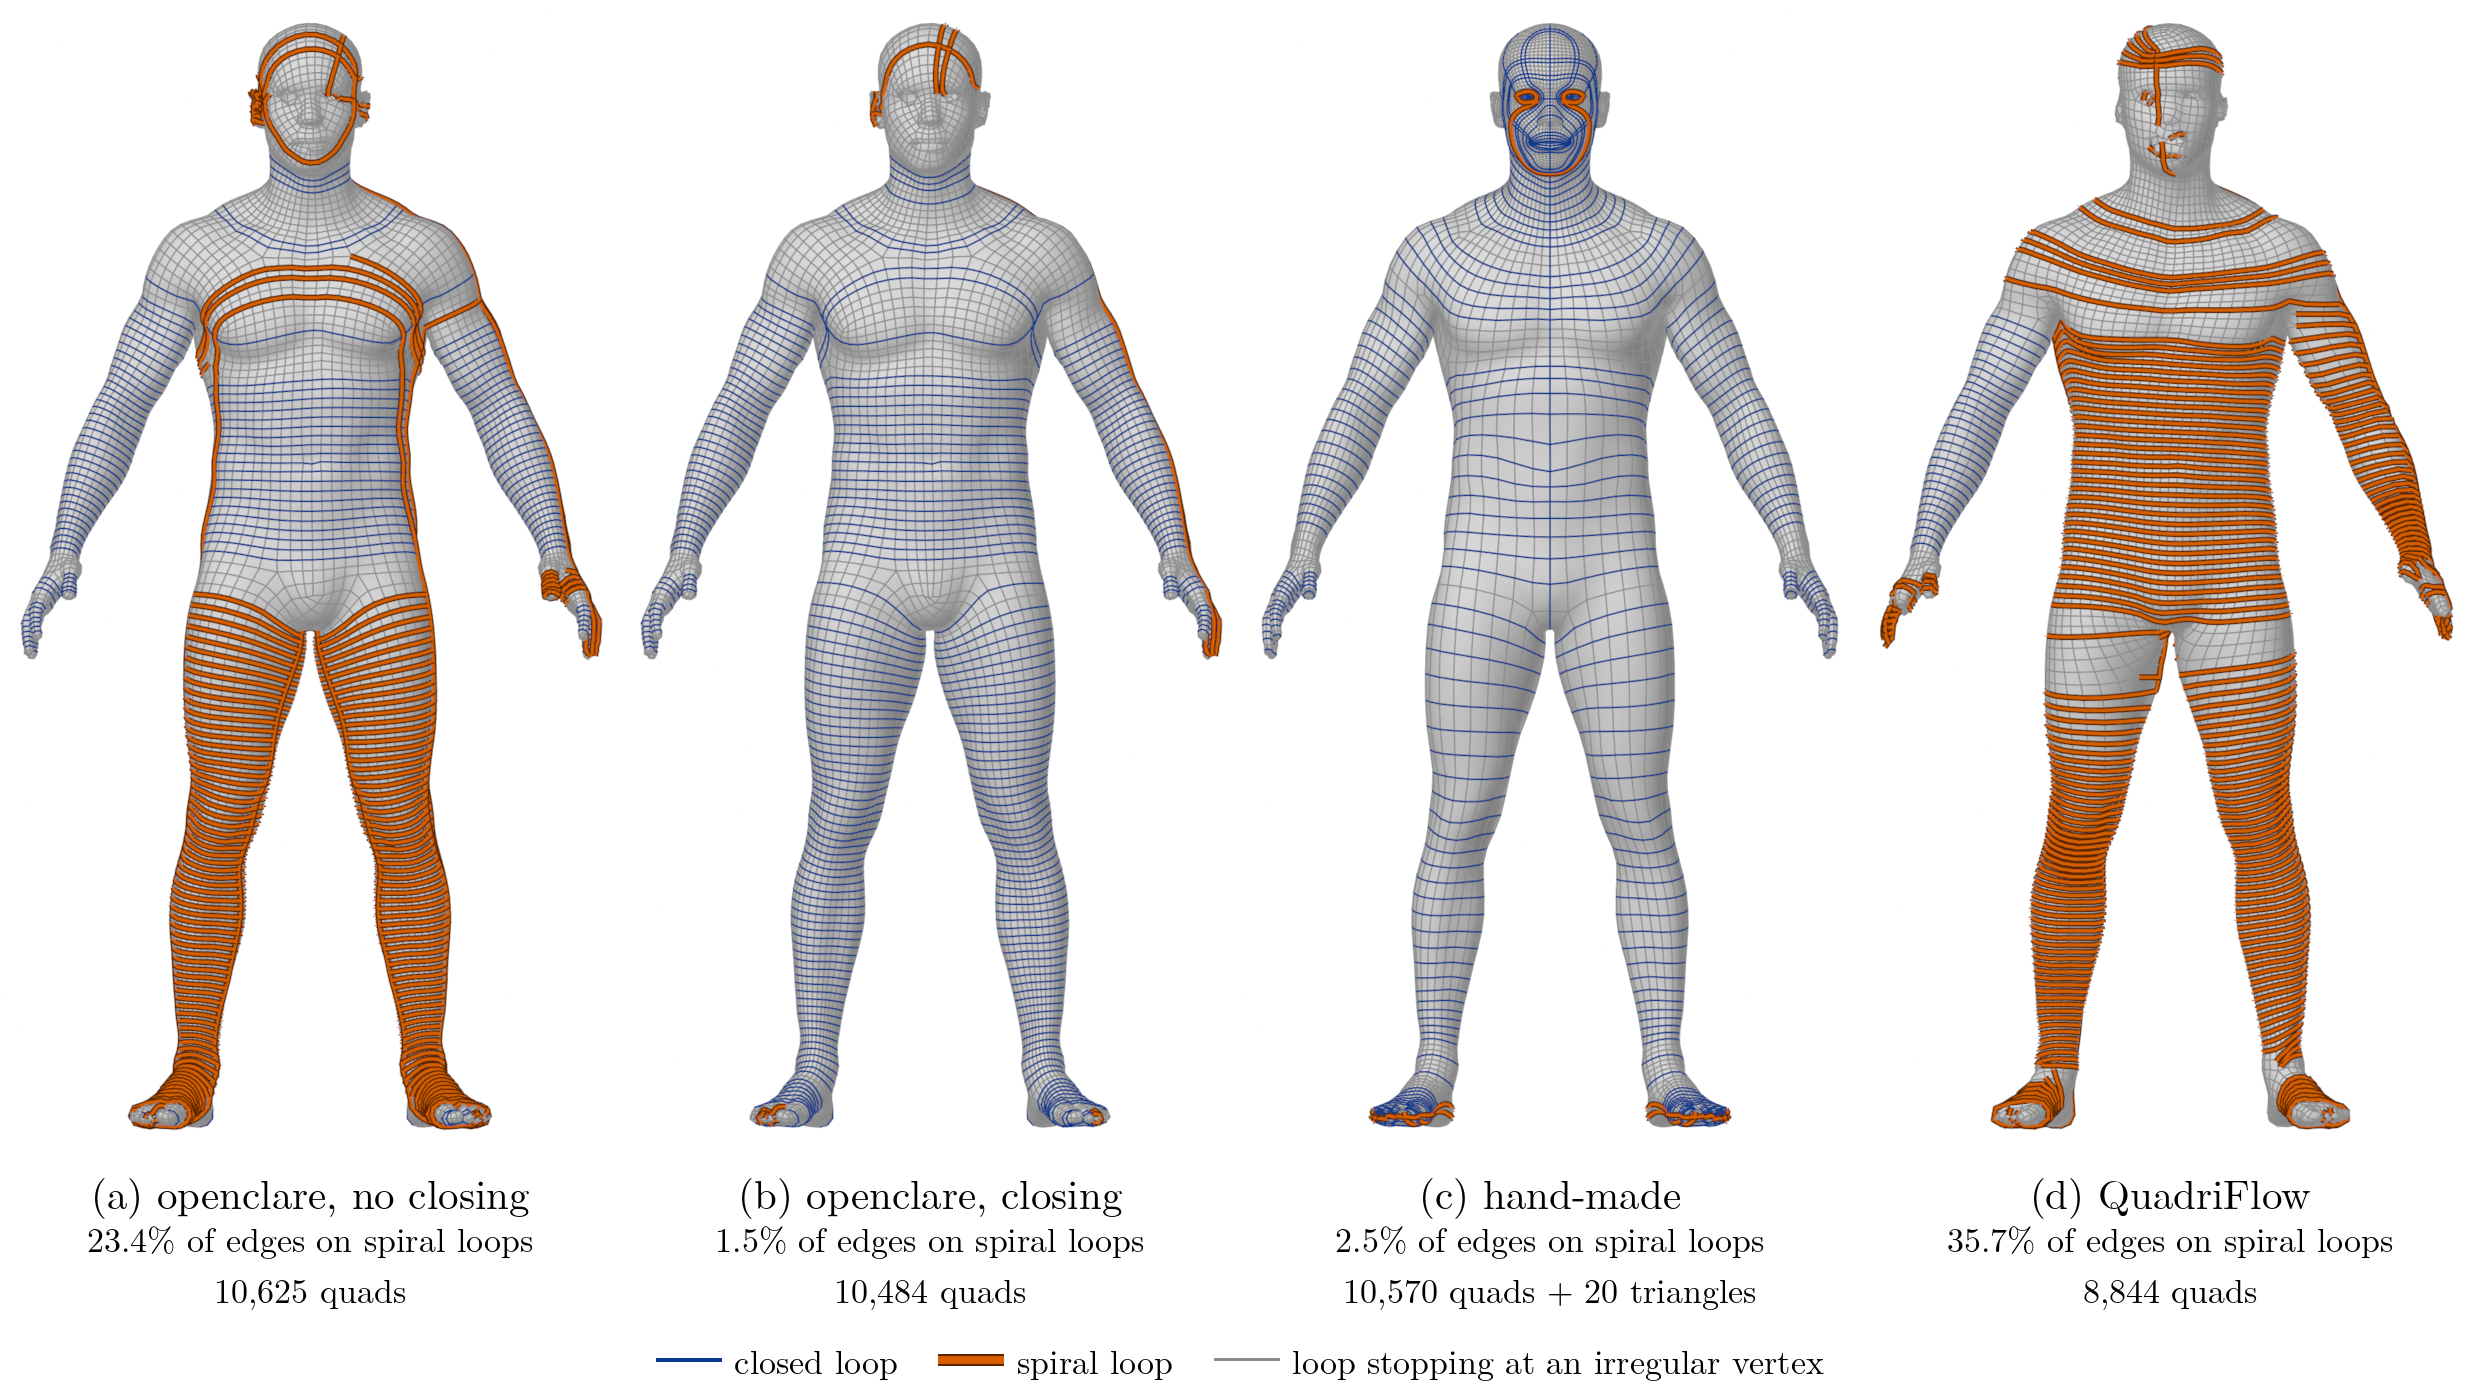
\includegraphics[width=\textwidth]{figures/male-overview.png}
\caption{The male body of the Essentials library, $10{,}590$ quads asked
for: (a)~openclare without closing, (b)~openclare with the closing of
Section~\ref{sec:closing}, (c)~the base mesh modelled by hand,
(d)~QuadriFlow run through Blender, on the source scaled by $100$ and scaled
back: Blender refuses the sculpt as it is, some of its edges being shorter
than its threshold of $10^{-4}$, and QuadriFlow does not depend on the scale.
Edge loops are coloured by their kind in
the measure of Section~\ref{sec:measure}: closed loops dark blue, spiral
loops vermillion (wider, with a dark rim), loops that stop at an irregular
vertex grey. Meshes (a) and (b) come from the engine of version 0.7.0, one
deterministic run each, the runs quoted in the text. Measured on the whole
meshes, they have $10{,}625$, $10{,}484$, $10{,}570$ (plus $20$ triangles)
and $8{,}844$ quads, $23.4\%$ ($21$ loops), $1.46\%$ ($11$), $2.55\%$ ($3$)
and $35.7\%$ ($43$) of their edges on spiral loops, which the panels round to
one decimal, and $17.2\%$, $36.5\%$, $31.6\%$ and $2.7\%$ on closed loops.
QuadriFlow's mesh has $3$ inverted faces and a Hausdorff distance of
$31$\textperthousand\ of the diagonal.}
\label{fig:overview}
\end{figure*}

\begin{figure*}[t]
\centering
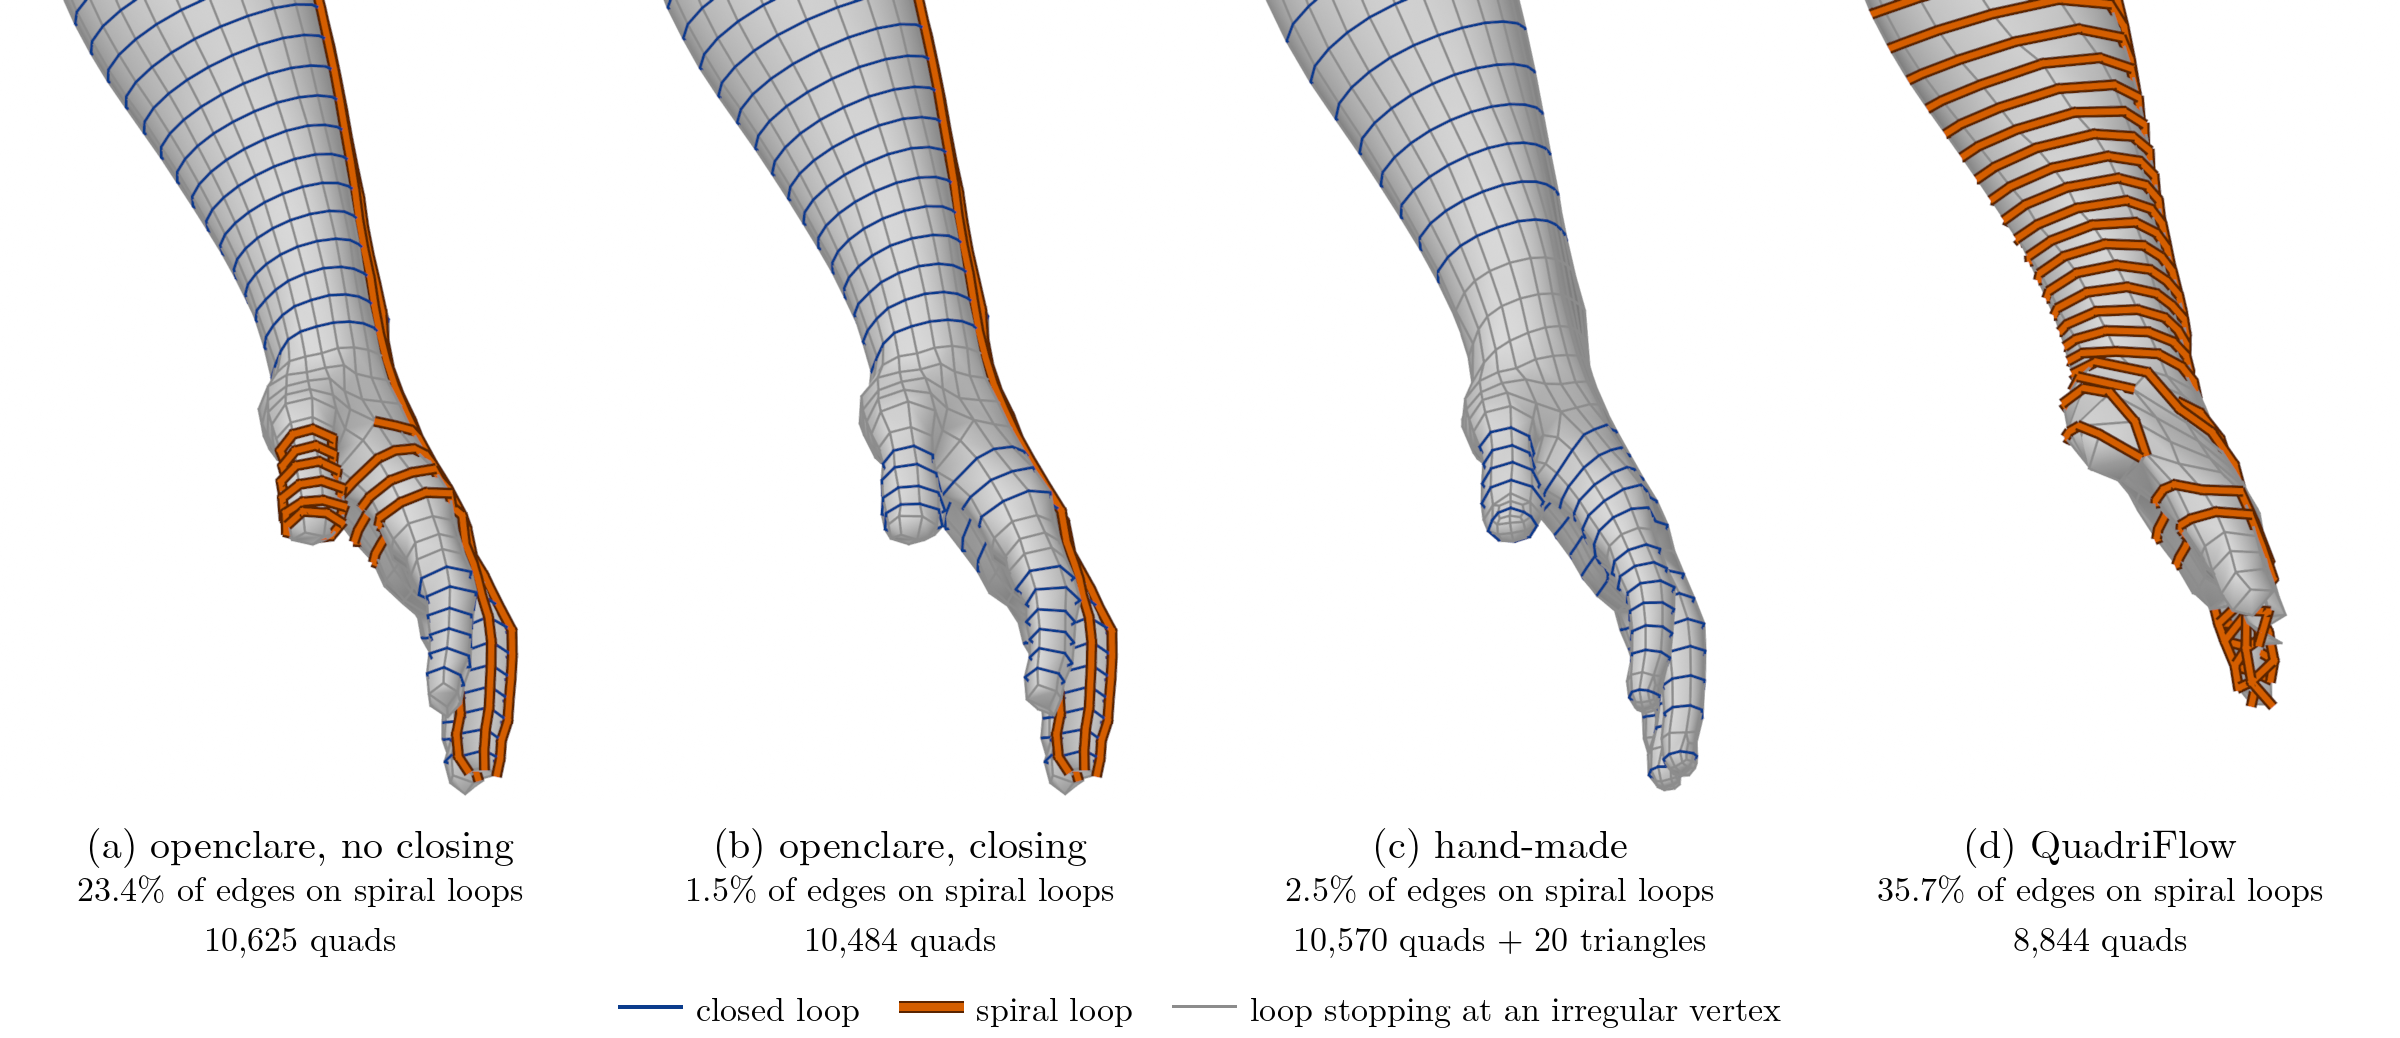
\includegraphics[width=\textwidth]{figures/male-wrist.png}\\[0.6em]
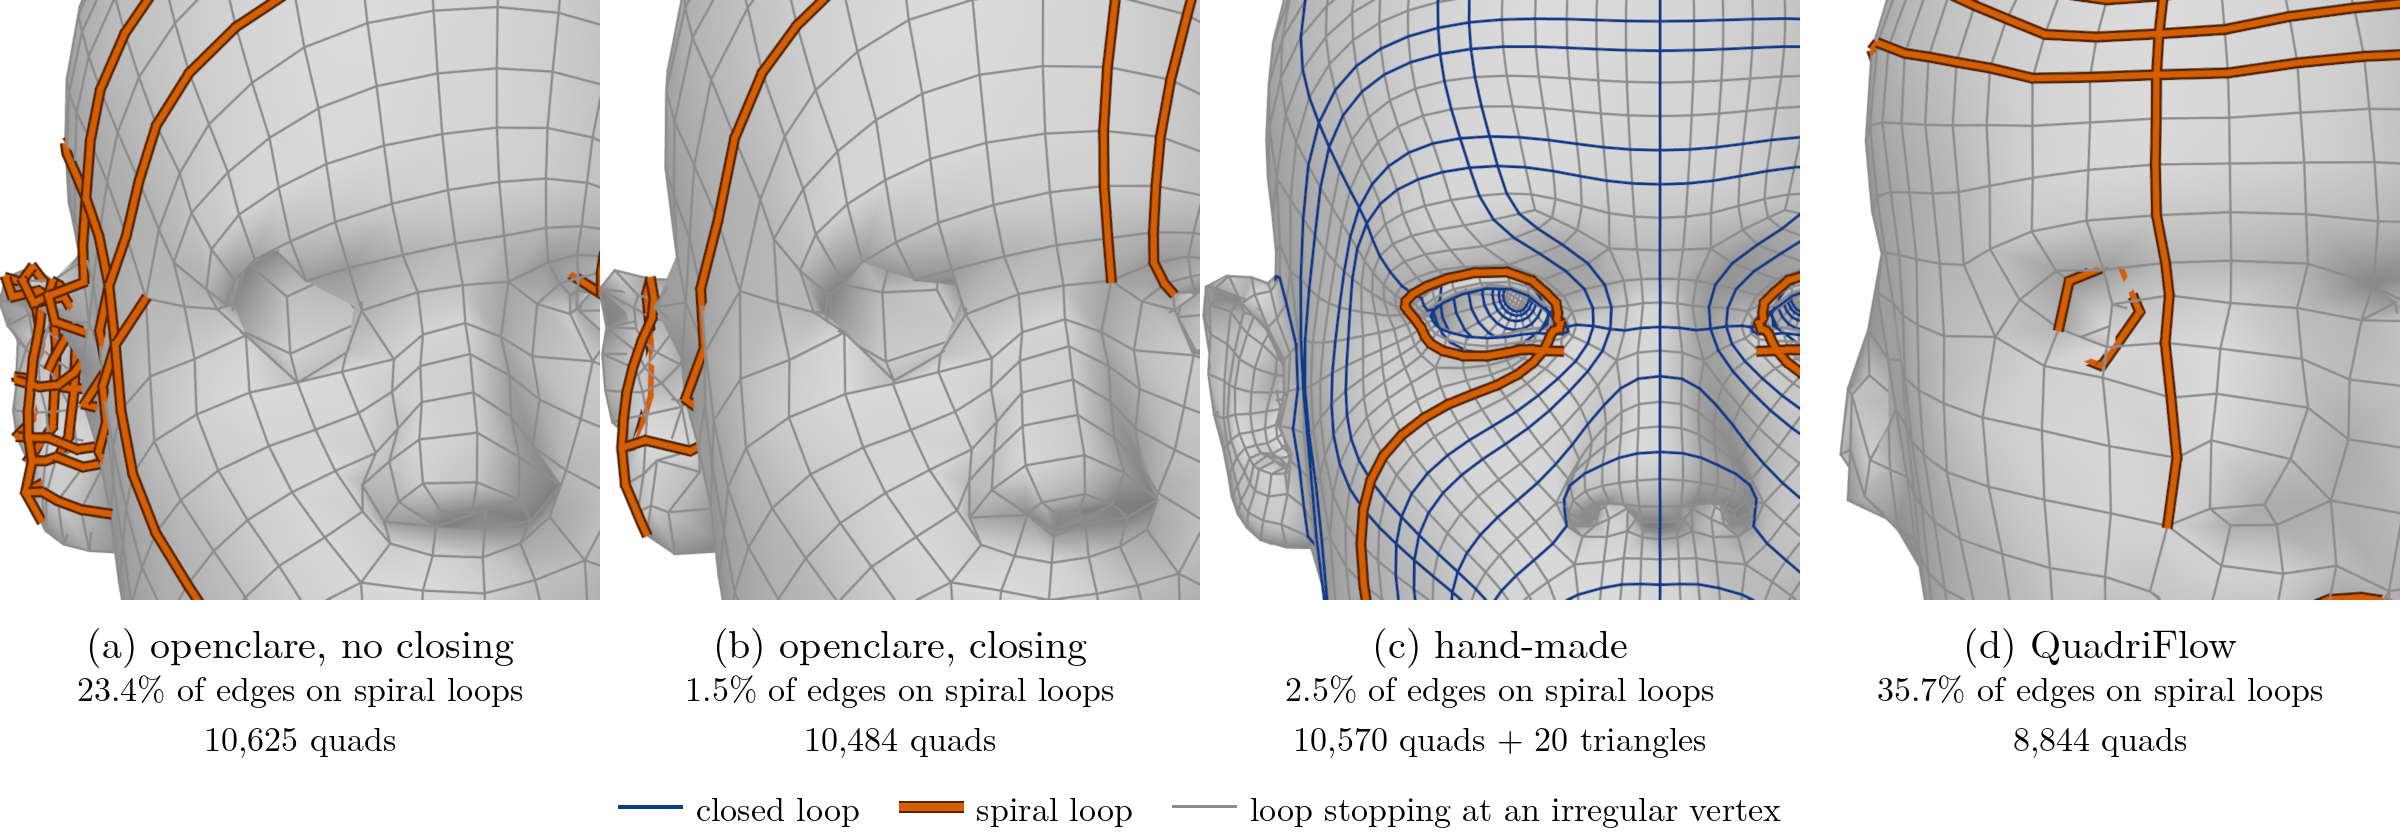
\includegraphics[width=\textwidth]{figures/male-eye.png}
\caption{Close-ups of the four meshes of Figure~\ref{fig:overview}, in the
same order and colours: the left wrist and hand (top; the body's left, on
the viewer's right in Figure~\ref{fig:overview}) and the right eye
(bottom). At the wrist, mesh~(b) has closed loops on the thumb and the back
of the hand where mesh~(a) has spiral ones, and a spiral loop along the outer
side of the forearm remains on both. At the eye, neither openclare mesh has
a spiral loop near the eye, both keep spiral loops on the forehead and at the
ear, and the loop round the eye of the hand-made mesh is itself counted as
spiral.}
\label{fig:closeups}
\end{figure*}

\section{An exact look at the closing system}\label{sec:exact}

How far is the heuristic of Section~\ref{sec:closing} from what the
constraints allow? An experiment option of the engine exports, for each way
of finding turns, the system it works on; we export it for the male body at
$10{,}590$ quads, from the engine as it runs. Its T-mesh has $1{,}342$ nodes
($1{,}068$ T-junctions, $254$ singular vertices, $131$ of valence three and
$123$ of valence five, and $20$ corners of folds), $2{,}146$ arcs and $806$
patches, hence $1{,}612$ balance equations, one per patch and direction. The
export gives the real lengths, every turn found with its shift (on all
$1{,}708$ turns, composing the crossing maps along the walk gives the
exported shift), and the lower bounds the integer search placed on arcs to
keep singularities apart ($36$ to $197$ arcs held at length one, depending on
the way). These bounds are the engine's choice of
\emph{which} arc of a chain between two singular vertices carries their
separation: validity asks a chain to keep a positive total length, not a
given arc. Every statement below is relative to them. We call
$P_{\mathrm{eng}}$ the balanced lengths that meet them; it is neither a
subset nor a superset of the valid quantizations, since it excludes valid
lengths that put the separation on another arc of the chain and allows
lengths that bring other arcs to zero. The ways are numbered as exported:
way $m + 2j + 4i$ starts from the shares $\{0.5\}$ ($m = 0$) or $\{0.2, 0.5,
0.8\}$ ($m = 1$), with the lean bound $0.05$ ($j = 0$) or $0.12$ ($j = 1$)
and the length bound $2$ ($i = 0$) or $6$ ($i = 1$) sides. Without the
other draws the engine keeps way~2 for this body ($1.65\%$ of spiral edges);
with them it keeps the lengths of another draw ($1.46\%$).

\paragraph{The conflict is real but local.}
All held turns can be closed together if the lengths are only asked to be
non-negative; with the bounds of separation, they cannot. By Farkas' lemma a
set of turns cannot be closed within the bounds exactly when some
combination of their shifts equals, modulo the balances, a non-negative
combination of arc lengths that charges an arc held open, and the companion
paper~\cite{gardent2026turns} reads these certificates on the singularities.
In seven ways (all but way~4) some held turn cannot even be closed on its
own. In five of them (0, 1, 2, 5 and 7) it is the same turn, of length
$6.76$, whose shift equals, modulo the balances, $-(\ell_{1892} +
\ell_{1908})$, where arc $1908$, less than $0.09$ quad edges long in the
parametrization, is held at length at least one; in ways 2, 3, 6 and 7 a
second turn, of length $4.72$, is held up in the same way by arc~$1006$ (both
certificates checked in exact rational arithmetic).
Whether $\ell_{1908} = 0$ would merge two singular vertices, that is whether
every valid quantization meets this bound, we did not check. Giving up the
least total amount of the bounds needed to close all held turns, a linear
program, shows that in way~0 the bound of arc $1908$ alone stands in the
way, in way~2 three bounds, that one among them, and in the other ways $6$
to $154$.

\paragraph{How many held turns can close.}
With every bound kept, the largest set of held turns that can be closed
together is found by a mixed-integer program with one binary per turn
(Table~\ref{tab:exact}). The projection of the engine keeps every held turn
closed: its active set asks the lengths to be non-negative only, which, as
above, lets all held turns close; the bounds of separation return in the
integer search. In whole numbers, the same mixed-integer program, with a
limit of fifteen minutes a way, proves its optimum in way~3 only ($90$
turns, as in real numbers); in the other ways it stops with $1$ to $88$
turns fewer than in real numbers.

\begin{table}[t]
\centering
\begin{tabular}{lrr}
\toprule
way & held & closable together \\
\midrule
0 & 58 & 57 \\
1 & 92 & 87 \\
2 & 64 & 61 \\
3 & 102 & 90 \\
4 & 125 & 120 \\
5 & 219 & 189 \\
6 & 131 & 123 \\
7 & 229 & 192 \\
\bottomrule
\end{tabular}
\caption{Male body at $10{,}590$ quads, real numbers, engine of version
0.7.0. ``Closable together'': the largest set of held turns closable with
every bound of separation kept; in way~7 the program stopped at its limit
of $300$ seconds, with a bound of $195$.}
\label{tab:exact}
\end{table}

\paragraph{The rounding ignores the shifts.}
Feeding the integer search of the engine better targets shows what survives
it (Table~\ref{tab:rounding}). The active-set projection, the engine's,
keeps every held turn closed in real numbers, yet after the integer search
$33\%$ to $74\%$ of them are shifted again ($170$ of $229$ in way~7); with a
least-squares projection whose negative lengths are clamped to zero, too,
about $40\%$ of the turns it closes are shifted after the integer search.
The integer search follows the targets but not the shifts. Aiming at the
lengths of the linear program, whose weighted $L^1$ objective puts the
changes on few arcs, the engine ranks first a candidate with $2.63\%$ of
spiral edges, yet outputs the mesh of the plain lengths: after meshing, the
candidates ranked before them were set aside.

\begin{table}[t]
\centering
\small
\begin{tabular}{lrrr}
\toprule
targets of the integer search & turns closed in reals & still shifted after & spiral edges (mesh) \\
\midrule
projection, clamped & 41--52 & 15--25 of them & 2.11\% \\
linear program, $L^1$ & 57--192 & 14--133 of them & 23.39\% \\
active set, floor 0 (the engine) & all held (58--229) & 19--170 of them & 1.46\% \\
active set, floor half the real length & 51--132 & 19--93 of them & 2.80\% \\
\bottomrule
\end{tabular}
\caption{Male body at $10{,}590$ quads, engine of version 0.7.0 with its
experiment options, one run each; ranges over the eight ways. The mesh keeps
the candidate with the fewest spirals, so its share is that of a single way
or draw; with the linear program it is the mesh of the plain lengths.}
\label{tab:rounding}
\end{table}

\paragraph{Whole lengths are not what is missing.}
The balances are the incidence matrix of a bidirected graph whose nodes are
the balance equations and whose edges are the arcs (each arc lies on a side
of each of the two patches it borders). When this graph is connected and has
a cycle that $\pm1$ values cannot balance, as on the body, the companion
paper shows that a set of free arcs parametrizes the lattice of whole
balanced lengths: here $2{,}146 - 1{,}612 = 534$ arcs can be given any whole
lengths and the others follow, so balances alone never obstruct whole
lengths. Closing exactly, in whole numbers, the turns found closable
together, HiGHS finds such lengths in $83$ to $228$ seconds in ways 0 to 3,
and none within ten minutes in ways 4 to 7. The solutions leave $1$, $5$,
$3$ and $12$ held turns shifted where the engine leaves $19$, $40$, $23$ and
$52$, and fewer of the turns not held as well ($3$ against $15$, $9$ against
$25$, $5$ against $18$, $11$ against $34$), at a weighted deviation from the
real lengths $2\%$ to $64\%$ higher. Yet three of the four spiral
\emph{more}, by the engine's count on the connectivity of their lengths:
$5.9\%$, $2.8\%$ and $7.8\%$ of their edges against $4.1\%$, $1.7\%$ and
$3.5\%$ for the engine's lengths in ways 0, 2 and 3; in way~1, $4.9\%$
against $9.1\%$. Only those of way~2 stay within the engine's window of
sizes; the others have $10{,}857$, $12{,}420$ and $11{,}011$ quads. Most of
the loops that spiral are not turns the sampled walks find.

Walking every strip of the mesh of way~2 instead
(Proposition~\ref{prop:complete}) finds $306$ ways round, each strip twice,
once in each direction; $236$ come back shifted. Selecting them by lean, as
the constraint rounds do, keeps $298$, of which $270$ ($135$ strips) can be
closed together in real numbers with every bound kept. Posed directly to
HiGHS, they gave no whole solution in $12{,}651$ seconds; given the $341$
arcs that every real solution sets to zero (each certified by a non-negative
combination of shifts, $216$ certificates over $36$ distinct sets of rings),
none was found in $2{,}596$ seconds either. No real lengths closing the
$270$ rings have a mean deviation from the targets below $1.304$, where the
engine allows $0.522$ ($0.2$ above the $0.322$ of its plain search). The
largest subset closable within a mean deviation of $0.4$, the number of
quads held to first order, found by a program stopped after $600$ seconds,
has $228$ rings (at most $267$) and closes at $0.395$ in real numbers. In
whole numbers, with the reformulation of Aardal, Hurkens and
Lenstra~\cite{aardal2000diophantine} on an LLL-reduced
basis~\cite{lenstra1982lll} of the lattice of closed quantizations, HiGHS,
stopped after $1{,}200$ seconds, finds whole lengths closing all $228$
within every bound at a mean deviation of $0.535$ and $10{,}653$ quads, and
proves that none does better than $0.518$. These lengths lie above the
engine's cap ($0.535$ against $0.522$), so the engine does not take them as
a candidate. Rounding costs between $0.123$ (proven) and $0.140$ (found) of
mean deviation above the real optimum.

\paragraph{The heuristic leaves most of the gap.}
The companion paper~\cite{gardent2026turns} computes the least number of
held turns that any lengths in $P_{\mathrm{eng}}$ leave shifted, a minimum
cover of the irreducible infeasible subsystems~\cite{parker1996iis}: exactly
$1$, $5$, $3$, $12$, $5$, $30$, $8$ and $37$ in ways 0 to 7, against $19$,
$40$, $23$, $52$, $61$, $154$, $72$ and $170$ left shifted by the engine.
With the engine's cap on the deviation and its window of sizes ($10{,}379$
to $10{,}801$ quads) added, at whole lengths, the least number is still
exactly one in way~0 and three in way~2: whole lengths closing every other
held turn exist at $10{,}730$ and $10{,}435$ quads, at mean deviations
$0.387$ and $0.506$. Of the $23$ turns of way~2 the engine leaves shifted,
the bounds of separation force three and the cap, the size and integrality
none; the heuristic accounts for $20$. Closing more turns, however, is not
what the measure of spirals sees: a local search over whole lengths within
the same cap and size closes $45$ more strips of the mesh of way~2 than the
engine does, but at its lengths, where the strips are other walks, $4.7\%$
of the edges spiral, against $1.7\%$ at the engine's lengths of way~2; it is
the choice of the turns to close, at the lengths where they are the strips
of the mesh, that decides how much the mesh spirals. Choosing the most turns to close
is NP-hard for bidirected balances with $0$--$1$ bounds, the algebraic form
of quantization~\cite{gardent2026turns}; whether the balances and turns of an
actual T-mesh stay hard is open.

\paragraph{Closing the most rings, end to end.}
We measured what an exact selection buys on the bench with the slow quality
mode of the engine (\texttt{--quality slow}), against the engine without its
other draws ($5.85\%$ of spiral edges over the $36$ runs), with three
($5.43\%$) and with its twelve ($4.92\%$). For the lengths the engine keeps,
a mixed-integer program closes as many of its strips leaning less than
$0.12$ as it can, weighted by their length round, within the balances, the
bounds of separation, the cap and the quad budget. A strip counts as closed
only where the corridor inequalities~\eqref{eq:corridor} hold for it, so
that it keeps its walk at the new lengths. The engine meshes the result, the
strips are walked again at the new lengths, and the program solved again,
three rounds; each round's lengths join the engine's candidates on the same
terms. The program is solved by HiGHS linked into the engine, each solve
stopped at a work limit (simplex iterations times arcs) that does not depend
on the load. Without the other draws, the slow mode lowers the mean to
$4.41\%$: lower on $9$ of the $36$ runs, never higher. Closed loops ($36.6\%$
against $35.4\%$ of the edges) and mean distance ($0.382$\textperthousand\
in both) barely move, and all $36$ meshes are valid. Against the twelve
other draws it is lower on average ($4.41\%$ against $4.92\%$) but not run
by run: higher on $9$ runs, lower on $5$. On the male body its three rounds
return the lengths they start from: $1.65\%$, as without it, against
$1.46\%$ for the engine with its draws. The gain does not need a solver that
finishes: $90$ of the $120$ solves stop at the work limit, and with a limit
of $5$ seconds per solve instead, $76$ of $100$ stop at it, $18$ of the $66$
rounds (against $12$) return the lengths they start from, and the mean is
$4.56\%$, on four processors where the other runs had eight.

\paragraph{Acting before quantization.}
Moving singular vertices in the parametrization, and rotating the field
cylinder by cylinder, were also tried, with prototypes of the engine that are
not part of it; neither lowered the share of spirals. The Burgers sum of the
companion paper~\cite{gardent2026turns} accounts for it: the shifts of two
parallel turns differ by the across component of the Burgers vector of the
singular vertices between them, which depends only on their developed
positions, so closing one turn by a local change of the map moves its shift
onto the turns beside it. The conflicts are better attacked in quantization.

\section{Limitations and open problems}\label{sec:limits}

The results come from one implementation and are preliminary. The spiral
share of a single model is chaotic, so only the means over three budgets are
robust; the other figures are single runs. The measure sees helices of pitch
up to four only. The exact look covers one body and holds relative to the
engine's bounds of separation, which are its choice of arcs and neither a
subset nor a superset of the valid quantizations. The machine was shared:
its load is recorded, not controlled, and the outcomes that depend on a
time limit depend on it.

Three problems remain open. \emph{An exact formulation}: minimizing the
deviation subject to the balances, the bounds and $\shift_\gamma(\ell) = 0$
for a set of turns is a minimum-deviation flow with linear side constraints;
how much of the exact machinery of~\cite{heistermann2023bimdf} carries over is
open, and the linear relaxation already closes $84\%$ to $98\%$ of the held
turns.
\emph{Closing in whole numbers}: whole lengths closing every ring asked for
are found through a reduced lattice basis, but in minutes, with the number
of quads held only to first order and $0.12$ to $0.14$ above the real optimum
in deviation, here above the engine's cap; can the integer search move within this lattice at the speed of
a flow solver? \emph{Which turns}, the central one on the evidence of
Section~\ref{sec:exact}: closing rings changes the lengths, the lengths
change the strips, and the strips of the new mesh are other walks. Is there a
finite set of turns whose closing implies that every loop of the quad mesh
closes? Can the loops of the quad mesh be read off the T-mesh and its lengths
directly, so that every one is accounted for? Which objective, short of all
loops, predicts the spirals the measure sees?

\section*{AI assistance}
This note and the software it describes were made by a human author working
with an AI system, which is not an author. The author chose the problem and
its aims (edge loops that close into rings and, as an artist, few singular
vertices and few spirals rather than perfectly square quads, quads only), set
the direction and the order of the work, decided which results to pursue and
which changes to merge, and judged the results through the measurements,
pictures and drafts presented to him. Claude Opus 5.5 (Anthropic), used
through Claude Code in October 2026 with several sub-agents in parallel,
wrote the changes to the engine and the experiment scripts, ran all the
experiments and exact computations, searched the literature, stated and
proved the propositions, and drafted the text. References were checked for
existence, and the note of each bibliography entry says how much of the work
was read. A work of which only the abstract, or a review, was read is cited only for what that abstract or review states. Weaker forms of Propositions~\ref{prop:linear}
and~\ref{prop:complete} are checked in Lean~4~\cite{demoura2021lean4} in the
companion paper, as the tag above each says; everything else here not checked by machine was written
with AI help and checked by AI agents rereading it and testing it on the
data, not by a human expert. The note has not been peer reviewed; the author,
who publishes it, is responsible for its content.

\bibliographystyle{plainnat}
\bibliography{refs}

\appendix

\section{Provenance of the figures}\label{app:provenance}

Every figure comes from the engine of version 0.7.0 (commit
\texttt{e13fadb}), built in release mode, and from the scripts of
\nolinkurl{docs/research/closing-loops/experiments/} (those of
Section~\ref{sec:exact} in its folder \nolinkurl{exact/}) and, for the
census, the conflicts and the least number of turns left shifted, which the
companion paper shares, of \nolinkurl{docs/research/turns-of-a-t-mesh/experiments/}.
Each script writes a summary, \texttt{results/}\textit{name}\texttt{.json}
beside it, with the engine's commit and build, the machine, its load and the
solver's version; its README gives the command of every table. The raw
output (meshes, exports, logs) is not in the repository.

\begin{center}
\small
\setlength{\tabcolsep}{4pt}
\begin{tabular}{@{}>{\raggedright\arraybackslash}p{5.6cm}>{\raggedright\arraybackslash}p{4.6cm}>{\raggedright\arraybackslash}p{4.4cm}@{}}
\toprule
figures & script & summary \\
\midrule
twelve models, three budgets (Section~\ref{sec:experiments})
  & \texttt{twelve\_models.py}, the protocol below
  & \texttt{twelve\_models.json} \\
Table~\ref{tab:dev}
  & \texttt{ablation.py}; its last line gave the $36$ meshes above byte for
  byte
  & \texttt{ablation.json} \\
against other remeshers
  & \texttt{against\_remeshers.py}, from \nolinkurl{bench/results/results.json}
  at \texttt{e13fadb}
  & \texttt{against\_remeshers.json} \\
male body, openclare and hand-made
  & \texttt{male\_body.py}
  & \texttt{male\_body.json} \\
Figures~\ref{fig:overview} and~\ref{fig:closeups}, their numbers
  & \texttt{figures/make\_figures.sh}, \texttt{figure\_numbers.py};
  QuadriFlow through Blender, on the source scaled by $100$ and scaled back
  & \texttt{figures.json} \\
Section~\ref{sec:exact}: the T-mesh, the conflicts, the least numbers left
shifted
  & \texttt{census.py}, \texttt{holonomy.py}, \texttt{conflicts.py},
  \texttt{forced.py} of the companion paper
  & their summaries of the same names \\
Section~\ref{sec:exact}: the other figures and Tables~\ref{tab:exact}
and~\ref{tab:rounding}
  & \texttt{exact/}: \texttt{relaxation.py}, \texttt{most\_closable.py},
  \texttt{rings.py}, \texttt{lattice\_rounding.py}, \texttt{local\_search.py},
  \texttt{remesh.py}
  & their summaries of the same names \\
closing the most rings, end to end
  & \texttt{exact/end\_to\_end.py}
  & \texttt{end\_to\_end.json}; the limit of $5$ seconds:
  \texttt{end\_to\_end-time-5.json} \\
\bottomrule
\end{tabular}
\end{center}

\paragraph{The protocol of the twelve models.} For each model $m$ (creature,
blob, suzanne, spot, pig, ogre, bob, jerry, blub, rock with the preset
\texttt{organic}; cage and part with \texttt{hard-surface}) and each budget
$Q \in \{2{,}970, 3{,}000, 3{,}030\}$: \texttt{openclare remesh}
\texttt{bench/out/}$m$\texttt{/source.obj} \textit{out.obj}
\texttt{--preset} $P$ \texttt{--quads} $Q$, then \texttt{openclare measure}
on the source and the output with \texttt{--target} $Q$ \texttt{--json}; the
figures are the means of \texttt{loop\_edges\_spiral},
\texttt{loop\_edges\_closed}, \texttt{loops\_spiral},
\texttt{mean\_distance} and \texttt{angle\_deviation\_mean} over the $36$
runs.

\paragraph{Reproducibility.} The method is implemented in openclare (Rust),
in the main branch of the repository; the bench is driven by
\texttt{bench/run.py}. The export of the T-mesh and the switches of
Table~\ref{tab:dev} are experiment options of the engine of version 0.7.0
(\texttt{ALGORITHM.md}, ``Experiment options''), and the slow quality mode
is its option \texttt{--quality slow}, so the scripts above make every
figure again on that engine; the figures that
depend on a time limit depend on the machine and its load as well. The
prototypes of ``Acting before quantization'' are not part of the engine and
are not scripted. This version of the note was built from commit
\texttt{\enginecommit}.

\end{document}
 gives the paper
% without them, for a venue that wants it plain.
\newcommand{\lean}[1]{\texttt{\detokenize{#1}}}
\ifdefined\plain
\newenvironment{evidence}[3][]{}{}
\else
\usepackage[most]{tcolorbox}
\newcommand{\evlevel}[2]{\expandafter\newcommand\csname ev-name-#1\endcsname{#2}}
\evlevel{lean}{Lean, complete}
\evlevel{core}{Lean, algebraic core}
\evlevel{data}{Checked on the engine's data}
\evlevel{measured}{Measured}
\evlevel{prose}{Proof on paper only}
\evlevel{tested}{Conjecture, checked by computer}
\evlevel{cited}{Standard, cited}
\evlevel{open}{Open, no claim}
\newcommand{\evname}[1]{\csname ev-name-#1\endcsname}
\tcbset{evstyle-lean/.style={}, evstyle-core/.style={}, evstyle-data/.style={},
  evstyle-measured/.style={}, evstyle-tested/.style={}, evstyle-prose/.style={},
  evstyle-cited/.style={},
  evstyle-open/.style={frame hidden, borderline={0.4pt}{0pt}{black!45, dashed}}}
\newtcolorbox{evidence}[3][]{breakable, enhanced, colback=white,
  colframe=black!45, boxrule=0.4pt, arc=0pt, left=4pt, right=4pt, top=2pt,
  bottom=2pt, before skip=6pt, after skip=6pt, evstyle-#2,
  title={\footnotesize\textsc{\evname{#2}}\if\relax\detokenize{#3}\relax\else
    \quad #3\fi},
  coltitle=black, colbacktitle=white, titlerule=0.4pt, toptitle=1pt,
  bottomtitle=1pt, #1}
\fi

\title{Closing Edge Loops at Quantization Time:\\
Helix Constraints for T-Mesh Quantization\\[0.5em]
\large Research note --- draft, not peer reviewed}
\author{Marc Gardent%
\thanks{This note is distributed under the Creative Commons Attribution
4.0 International licence (CC BY 4.0). The code of openclare is under the
GPL-3.0-or-later of the repository. The note describes the engine at commit
\texttt{\enginecommit} of \url{https://github.com/marcgardent/openclare}.
A French translation is in \texttt{paper.fr.pdf}, beside this note.}\\
\normalsize Independent researcher\\
\normalsize ORCID: \href{https://orcid.org/0009-0000-6466-3098}{0009-0000-6466-3098}\\
\normalsize Contact: through the repository,
\url{https://github.com/marcgardent/openclare}}
\date{October 2026}

\begin{document}
\maketitle

\begin{abstract}
Automatic quad remeshing often produces edge loops that wind round a part of
the shape as helices instead of closing into rings. Bommes et
al.~\cite{bommes2011structure} remove such \emph{q-helices} from a finished
mesh; we prevent them where the integer structure of the mesh is decided, in
the quantization of a T-mesh. A straight walk across the patches of a T-mesh
that returns to its first side, a \emph{turn}, has a \emph{shift} that is an
integer linear form in the arc lengths; at whole lengths it is how far the
strip of quads following the turn comes back beside itself, and every strip
of the mesh is such a walk. We add the constraints that close turns to a
minimum-deviation quantizer~\cite{heistermann2023bimdf}, through a
least-change projection, repair walks and rounds of constraint generation on
the strips of the mesh, and keep the candidate with the fewest spiral edges,
counted by a test that tells helices from closed, open and border loops. Over
twelve models at three budgets near 3{,}000 quads, the engine leaves 4.92\%
of the edges on spiral loops (19.8\% without closing); on the seven models
that two other open-source remeshers also mesh validly, 2.2\% against 38.8\% % NIGHT4
and 21.7\%; on a human body, 1.5\%, against 2.5\% for the hand-made mesh.
An exact analysis of the closing system of that body shows that the conflict between closing
turns and keeping singularities apart is real but local, that the heuristic
rather than the constraints leaves most turns shifted, and that closing more
turns does not by itself make fewer spirals: the strips move with the
lengths, and the choice of the turns to close decides.
\end{abstract}

\section{Introduction}

In our experience, element shape and alignment are rarely what limits
field-aligned quad remeshing today (see the
surveys~\cite{bommes2013survey,campen2017survey}). What remains is structure:
the way edge loops run across the surface. Artists expect a loop round an
arm, a leg or a neck to be a ring. Automatic methods often produce a helix
instead: the loop goes round, comes back one or a few rows further, and winds
along the whole part (Figure~\ref{fig:overview}). Bommes et al.\ showed that
helical configurations are a main reason why the base complex of an otherwise
good quad mesh stays dense~\cite{bommes2011structure}, and removed them from
the finished mesh.

Whether a loop closes is decided upstream, when a quantizer assigns whole
lengths to the arcs of a T-mesh traced in a seamless
parametrization~\cite{campen2015qgp,lyon2021constrained,heistermann2023bimdf}.
Quantizers choose these lengths for consistency, validity and closeness to
the parametrization; the loops close or spiral as a side effect. This paper
constrains the loops in the quantization itself. Section~\ref{sec:turns}
defines \emph{turns}, straight walks across the patches of a T-mesh that
return to their first side, and shows that the \emph{shift} of a turn is an
integer linear form in the arc lengths that gives, at whole lengths, the
pitch of the strip of quads following it, and that every strip of the mesh
is such a walk. Section~\ref{sec:closing} adds the closing of turns to a
minimum-deviation quantizer through a least-change projection, repair walks
and rounds of constraint generation on the strips, with safeguards on folds,
distortion and budget. Section~\ref{sec:measure} gives a share of spiral
edges that tells helices of pitch up to four from closed, open and border
loops; loop counts and loop simplicity scores
exist~\cite{liu2025quadgpt,kong2026squadgen}, but they do not separate
helices from open loops. Section~\ref{sec:experiments} measures the method in
the open-source remesher openclare against two open-source remeshers and a
mesh modelled by hand, and Section~\ref{sec:exact} solves the closing system
of a human body exactly to see where the heuristic stands: the conflict
between closing turns and keeping singularities apart is local, the
heuristic leaves most of the shifted turns that no constraint forces, and
yet closing more turns does not by itself reduce the spirals, because the
strips of the mesh move with the lengths; adding the inequalities of the
corridor makes the count of closed strips exact, a coupling of shift and
corridor we found in no earlier quantizer. Section~\ref{sec:limits} states
the limitations and the open problems.

This work began as a programming project, openclare, an open-source quad
remesher, and became research when engineering alone could no longer tell
which results could be guaranteed and which computations could be saved.
Each result used here answers such a question. The shift of a turn is linear
in the arc lengths, so closing a loop becomes a linear constraint of the
quantizer rather than a test after the fact; its parity follows the length
of the turn, so some repairs are known to be impossible before they are
tried; and choosing the largest set of turns to close is NP-hard in the
algebraic form quantization takes, which is why the engine keeps to a heuristic, with an exact solver only on demand.

The theory behind the conflicts, which reads the shift as translational
holonomy of the flat metric and derives obstructions to closing from the
singularities, a lower bound on the turns every quantization leaves shifted,
and the NP-hardness of choosing the turns to close, is the subject of a
companion paper~\cite{gardent2026turns}; we state its results in one
sentence where we need them, without proof. Statements here are
\emph{proved} when they come with a proof, \emph{measured} when they come
from exact arithmetic or solver output on the systems openclare exports, and
\emph{conjectured} otherwise.

\section{Background and related work}\label{sec:related}

\paragraph{T-mesh quantization.}
Mixed-integer quadrangulation~\cite{bommes2009miq} and integer-grid
maps~\cite{bommes2013igm} decide the integer structure of a quad mesh in
their quantization. Campen et al.\ show that even a valid quantization of a seamless
parametrization is a hard combinatorial problem, and solve it through
systems of linear Diophantine equations~\cite{campen2015qgp}.
Lyon et al.\ solve a constrained version as an integer linear program,
bounding the directional deviation of the separatrices of the resulting
layout, and require, as openclare does, that the quantization keep
singularities apart~\cite{lyon2021constrained}. Heistermann et al.\ cast
quantization as a minimum-deviation flow on a bidirected graph and give a
fast approximate solver and an exact refinement~\cite{heistermann2023bimdf};
openclare follows their formulation. To our knowledge none of these
constrains the helices.

\paragraph{Helices after meshing.}
Bommes et al.~\cite{bommes2011structure} define a \emph{q-helix} as a dual
parametric line with an integer \emph{pitch} $h$ and \emph{turn length}
$\tau$: walking $\tau$ steps along it is equivalent to $h$ side-steps. They
detect minimal q-helices by the self-intersections of orthogonal dual lines
and remove them greedily with grid-preserving operators, closed dual paths of
shift and collapse steps that keep the mesh all-quad and its singularities in
place, followed by tangential smoothing; their experiments remove most
helices (from 17--52 down to 1--23 per model). They note that choosing the
pairs of singularities to align directly in the parametrization is often
complicated or even ambiguous to automate, giving the feature-aligned
T-meshes of Myles et al.~\cite{myles2010feature} as an example. Razafindrazaka and
Polthier~\cite{razafindrazaka2017optimal} replace the base complex of a
finished mesh by an optimal one, found as a perfect matching on a graph over
its singular vertices, and note that the operators
of~\cite{bommes2011structure} leave some spirals. Both work after meshing,
not in the quantization.

\paragraph{Periods round a tube.}
QuadCover~\cite{kalberer2007quadcover} lifts the cross field to a branched
covering where it becomes a vector field. The stripe parameterization of
tubular surfaces~\cite{kalberer2011stripe}, built on it, measures the jump
(``gap'') of the parameter across each cut path and rounds it to the nearest
whole number; the gap across a loop round a tube is what we call the shift of
a turn, and rounded to a non-zero whole number it gives a helix of that
pitch. That paper treats spiralling stripes as a legitimate outcome, and
notes that rounding the gaps for least distortion is a hard combinatorial
problem that it does not solve exactly.

\paragraph{Flat metrics and finite trajectories.}
Declaring every quad a unit square turns a quad mesh into a flat metric with
cone points at its irregular vertices. Chen et al.~\cite{chen2019metric}
characterize the metrics that arise this way; one of their conditions is a
\emph{finite geodesic lamination}, the straight lines of the field being
finite loops, which they assume rather than construct. Lei et
al.~\cite{lei2020quartic} show that a closed quad mesh induces a meromorphic
quartic differential and list as an open problem the guarantee that all its
trajectories are finite. A trajectory that is not finite is precisely an edge
loop that does not close. A quadratic differential all of whose non-critical
trajectories close is a Jenkins--Strebel
differential~\cite{strebel1984quadratic}; the complement of its critical
graph is a union of flat cylinders, and a helix is a cylinder glued back with
a shift of a whole number of rows. On a closed surface the valences $k(v)$ of
a quad mesh satisfy $\sum_v (4 - k(v)) = 4\chi$: with valences three and five only, a
closed human body needs at least eight vertices of valence three, but a hand-made base mesh has
hundreds, and their count says nothing of where the loops go.

\paragraph{Loops by construction.}
Dual loops meshing~\cite{campen2012dual} builds a layout from loops traced on
the surface, which close by construction; Lei et
al.~\cite{lei2017foliation} build quad meshes from a Strebel differential
with prescribed cylinders, and skeleton-guided
layouts~\cite{usai2015skeleton} follow the curve skeleton of an articulated
shape. Myles
et al.~\cite{myles2014robust} trace the field into a partition into patches,
Pietroni et al.~\cite{pietroni2016tracing} extract a layout from traced
field-coherent paths with a binary linear program, and Razafindrazaka et
al.~\cite{razafindrazaka2015perfect} obtain a layout as a minimum-weight
perfect matching. These methods build coarse layouts, or, for Myles et al.,
a parametrization from one; none asks the loops of a dense mesh to close.

\paragraph{Measuring loops.}
QuadGPT~\cite{liu2025quadgpt} counts \emph{quad rings} (closed loops of
faces) and \emph{quad lines} (open strips) and uses them as reward signals
for preference optimization, without telling spirals from open lines.
SQuadGen~\cite{kong2026squadgen} scores the loops of a layout by their
self-intersections and their rotation index, and reports the area share of
simple loops; it does not tell helices from open loops either.

\section{Turns of a T-mesh}\label{sec:turns}

A T-mesh is a partition of the surface into rectangles, the \emph{patches},
whose sides are made of \emph{arcs}; nodes where a trace stops on another are
T-junctions, and the singular vertices of the field are nodes. Each patch
$P$ has local coordinates with its first corner at the origin and its sides
along the axes. A quantization assigns every arc $a$ a length $\ell_a \in
\Z_{\ge 0}$ such that opposite sides of every patch have equal length, the
\emph{balances} $B\ell = 0$; the quad mesh is then read off as the integer
grid of each patch.

\begin{definition}[Turn]
A \emph{turn} $\gamma$ is a straight walk across patches, from an offset of
its first side that meets no node: it enters a patch through a side, leaves
through the opposite side at the same distance from the corresponding
corner, enters the neighbouring patch across the arc it reaches, and so on,
until it comes back into its first patch through its first side.
\end{definition}

\begin{figure}[t]
\centering
% A turn of a T-mesh, its corridor, its shift and the helix it makes.
% \input inside a figure; needs \usepackage{tikz} and
% \usetikzlibrary{arrows.meta,decorations.pathreplacing}.
%
% (a) A band of a T-mesh on a cylinder, cut open along the left side of P_1:
% the right side of P_4 is glued to the left side of P_1, drawn again, dashed,
% where the walk comes back into it. The band continues above and below. Every
% node is at a whole position; the faint grid is the quad mesh at these
% lengths. The turn gamma starts on the left side of P_1 at offset o = 2.5 and
% crosses P_1, P_2, P_3, P_4. Measured from the first (lower) corner of each
% patch, its offset grows by l_b crossing into P_2, drops by l_c into P_3 and
% grows by l_d into P_4; the bottoms of P_4 and P_1 meet at the cut. So it comes
% back into P_1 at o + s with s = l_b - l_c + l_d = 1 - 2 + 2 = 1. The corridor
% (the offsets whose walk crosses the same arcs) is 1 < o < 4.
% (b) The strip of quads at o = 2.5 on the cylinder: each round comes back one
% row beside itself, at o = 1.5, 2.5, 3.5 within the corridor, then leaves it:
% a helix of pitch 1. The numbers are the offsets where the rounds start.
\begin{tikzpicture}[x=0.56cm, y=0.56cm, font=\small,
    side/.style={draw=black, line width=0.6pt},
    ghost/.style={draw=black!55, line width=0.6pt, dashed},
    quadgrid/.style={draw=black!18, line width=0.3pt},
    node dot/.style={circle, fill=black, inner sep=0pt, minimum size=3.2pt},
    arc mark/.style={line width=2.2pt, draw=black},
    turn/.style={line width=1.1pt, draw=black, -{Stealth[length=6pt]}},
    brace/.style={decorate, decoration={brace, amplitude=4pt}, line width=0.6pt}]
  \definecolor{corridor}{HTML}{CFE0F3}
  \definecolor{loopspiral}{HTML}{D55E00}

  % ---------------------------------------------------------------- (a)
  \begin{scope}
    \clip (-0.1,-2.4) rectangle (16.1,7.4);
    % The corridor of the turn, 1 < o < 4, from P_1 round to P_1 again.
    \fill[corridor] (0,1) rectangle (13,4);
    \draw[quadgrid, step={(1,1)}] (0,-3) grid (16,8);
    % Sides of the columns of patches, which run through the band.
    \foreach \x in {0,3,7,10,13} \draw[side] (\x,-3) -- (\x,8);
    \draw[ghost] (16,-3) -- (16,8);
    % The bottom and top of P_1, ..., P_4, and of P_1 again.
    \foreach \x/\X/\b/\t in {0/3/0/5, 3/7/-1/4, 7/10/1/6, 10/13/-1/4} {
      \draw[side] (\x,\b) -- (\X,\b) (\x,\t) -- (\X,\t);
      \foreach \px in {\x,\X} \foreach \py in {\b,\t}
        \node[node dot] at (\px,\py) {};
    }
    \draw[ghost] (13,-1) -- (16,-1) (13,4) -- (16,4);
    \foreach \py in {-1,4} \node[node dot, fill=black!55] at (16,\py) {};
  \end{scope}
  % The arcs whose lengths the shift adds up.
  \draw[arc mark] (3,-1) -- (3,0) node[midway, left=1pt] {$b$};
  \draw[arc mark] (7,-1) -- (7,1) node[midway, left=1pt] {$c$};
  \draw[arc mark] (10,-1) -- (10,1) node[midway, right=1pt] {$d$};
  % Patch names.
  \node at (1.5,4.5) {$P_1$};
  \node at (5,0) {$P_2$};
  \node at (8.5,5) {$P_3$};
  \node at (11.5,0) {$P_4$};
  \node[black!60] at (14.5,3.35) {\footnotesize $P_1$ again};
  % The turn, from offset o = 2.5 of the first side of P_1.
  \draw[turn] (0,2.5) -- (13.08,2.5);
  \node[above] at (6.4,2.5) {$\gamma$};
  \draw[black, line width=0.6pt, fill=white] (0,2.5) circle (2.2pt);
  % Where it comes back: in the frame of P_1, at o + s.
  \draw[black!60, dashed, line width=0.8pt] (13,2.5) -- (16,2.5);
  \draw[black!60, dotted, line width=0.9pt] (13,1.5) -- (16,1.5);
  \draw[black, line width=0.6pt, fill=white] (13,1.5) circle (2.2pt);
  \node[right, inner sep=1pt] at (16.15,2.5) {\footnotesize $o + s_\gamma(\ell)$};
  \node[right, inner sep=1pt] at (16.15,1.5) {\footnotesize $o$};
  \draw[brace, decoration={mirror}] (15.7,1.5) -- (15.7,2.5)
    node[midway, left=4pt, inner sep=1pt] {\footnotesize $s_\gamma$};
  % Offset and corridor on the first side.
  \node[left] at (-0.05,2.5) {$o$};
  \draw[brace] (-0.9,1) -- (-0.9,4) node[midway, left=4pt, rotate=90, anchor=south]
    {\footnotesize corridor};
  % The shift as a linear form of the arc lengths.
  \node[anchor=north west] at (0,-2.7)
    {$s_\gamma(\ell) = \ell_b - \ell_c + \ell_d = 1 - 2 + 2 = 1$};
  \node[anchor=north] at (8,-4.2) {(a)};

  % ---------------------------------------------------------------- (b)
  % The strip of quads at o = 2.5 on the cylinder, seen from slightly above:
  % a helix of pitch |s| = 1 row, three rounds in the corridor, 13 quads a
  % round (the length of the turn).
  \begin{scope}[shift={(22.4,-1.6)}]
    \pgfmathsetmacro{\R}{1.9}   % radius
    \pgfmathsetmacro{\k}{0.2}   % flattening of the ellipses
    \pgfmathsetmacro{\w}{1.15}  % one row of quads
    \pgfmathsetmacro{\H}{7.0}   % height
    \pgfmathsetmacro{\zz}{1.4}  % bottom of the first round
    % Back halves: the centre line of the strip, seen through the cylinder.
    \foreach \j in {0,1,2} {
      \draw[loopspiral!80, dashed, line width=0.7pt]
        plot[domain=360*\j+180:360*\j+360, samples=40, variable=\t]
          ({\R*cos(\t)}, {\zz + \w*(\t/360 + 0.5) - \k*\R*sin(\t)});
    }
    % The cylinder, translucent.
    \fill[black!25, fill opacity=0.18] (-\R,0) -- (-\R,\H) arc[start angle=180, end angle=360,
      x radius=\R, y radius=\k*\R] -- (\R,0) arc[start angle=0, end angle=-180,
      x radius=\R, y radius=\k*\R] -- cycle;
    \draw[line width=0.6pt] (-\R,0) -- (-\R,\H) (\R,0) -- (\R,\H);
    \draw[line width=0.6pt] (0,\H) ellipse[x radius=\R, y radius=\k*\R];
    \draw[line width=0.6pt] (\R,0) arc[start angle=0, end angle=-180,
      x radius=\R, y radius=\k*\R];
    \draw[line width=0.4pt, black!40, dashed] (\R,0) arc[start angle=0, end angle=180,
      x radius=\R, y radius=\k*\R];
    % Front halves: the quads of the strip, 13 a round, and its centre line.
    \foreach \j in {0,1,2} {
      \fill[loopspiral!35, fill opacity=0.55]
        plot[domain=360*\j:360*\j+180, samples=40, variable=\t]
          ({\R*cos(\t)}, {\zz + \w*\t/360 - \k*\R*sin(\t)})
        -- plot[domain=360*\j+180:360*\j, samples=40, variable=\t]
          ({\R*cos(\t)}, {\zz + \w*(\t/360 + 1) - \k*\R*sin(\t)}) -- cycle;
      \foreach \e in {0,1} {
        \draw[loopspiral!70, line width=0.5pt]
          plot[domain=360*\j:360*\j+180, samples=40, variable=\t]
            ({\R*cos(\t)}, {\zz + \w*(\t/360 + \e) - \k*\R*sin(\t)});
      }
      \foreach \q in {1,...,6} {
        \pgfmathsetmacro{\t}{360*\j + \q*360/13}
        \draw[loopspiral!70, line width=0.4pt]
          ({\R*cos(\t)}, {\zz + \w*\t/360 - \k*\R*sin(\t)}) --
          ({\R*cos(\t)}, {\zz + \w*(\t/360 + 1) - \k*\R*sin(\t)});
      }
      \draw[loopspiral, line width=1.1pt, -{Stealth[length=5pt]}]
        plot[domain=360*\j:360*\j+176, samples=40, variable=\t]
          ({\R*cos(\t)}, {\zz + \w*(\t/360 + 0.5) - \k*\R*sin(\t)});
      % The offset on the first side where the round starts.
      \pgfmathsetmacro{\n}{\j + 1.5}
      \node[right, font=\scriptsize, inner sep=2pt] at (\R,\zz + \w*\j + 0.5*\w)
        {$\pgfmathprintnumber[fixed, precision=1, fixed zerofill]{\n}$};
    }
    \node[anchor=north, align=center, font=\footnotesize] at (0,-0.5)
      {the strip at $o = 2.5$: one helix\\ through $o = 1.5$, $2.5$, $3.5$,\\ pitch $|s_\gamma(\ell)| = 1$};
  \end{scope}
  \node[anchor=north] at (22.4,-4.2) {(b)};
\end{tikzpicture}

\caption{A turn and the helix it makes. (a)~A band of a T-mesh on a
cylinder, cut open along the first side of $P_1$, which is drawn again,
dashed, past $P_4$, where it is glued; every node is at a whole position and
the faint grid is the quad mesh at these lengths. The turn $\gamma$ leaves
the first side at offset $o$ and crosses $P_1$ to $P_4$; measured from the
first corner of each patch, its offset grows by $\ell_b$, drops by $\ell_c$
and grows by $\ell_d$, so it comes back at $o + \shift_\gamma(\ell)$ with
$\shift_\gamma(\ell) = \ell_b - \ell_c + \ell_d = 1$. The corridor
(shaded), the offsets whose walk crosses the same arcs, is $1 < o < 4$.
(b)~The strip of quads at $o = 2.5$ on the cylinder: each round comes back
one row beside itself, through $o = 1.5$, $2.5$ and $3.5$, then leaves the
corridor: a helix of pitch $1$ (Proposition~\ref{prop:linear}).}
\label{fig:turn}
\end{figure}

Crossing from patch $P$ to patch $Q$ across an arc composes a quarter-turn
rotation of the local frame with a translation whose components are signed
sums of arc lengths along the rims of $P$ and $Q$, the position of a rim
point being the sum of the lengths of the arcs between it and the first
corner.

\begin{evidence}{core}{\lean{TMesh.Turn.shift_linear}, \lean{TMesh.Turn.mem_corridor_iff}, \lean{TMesh.Turn.comes_back}, \lean{TMesh.Turn.winds}; examples: \lean{TMesh.twistedTorus.walk_turn}; assumed: an oriented gluing; the corridor without half-integers is not formalized}
\begin{proposition}[The shift of a turn is linear]\label{prop:linear}
For a turn $\gamma$ there are integer coefficients $c_a$, independent of the
lengths, such that after a full turn a point of the first side has moved
across the walking direction by
\[
  \shift_\gamma(\ell) = \sum_a c_a\, \ell_a .
\]
For whole lengths $\ell$, let $o$ be a half-integer offset of the first side
whose walk at the lengths $\ell$ crosses the same patches as $\gamma$ (the
set of such offsets is the \emph{corridor} of $\gamma$ at $\ell$). Then the
dual line of the quad mesh at $o$ comes back at $o + \shift_\gamma(\ell)$:
it closes after one round if and only if $\shift_\gamma(\ell) = 0$. If
moreover $o + j\,\shift_\gamma(\ell)$ lies in the corridor for $j = 1, \dots,
t - 1$, it winds $t$ times round as a helix of pitch $|\shift_\gamma(\ell)|$
in the sense of~\cite{bommes2011structure}.
\end{proposition}
\end{evidence}

\begin{proof}[Sketch]
Each crossing is a map $x \mapsto R^k x + t$ with $R$ the quarter-turn and
$t$ a vector whose entries are sums of $\pm\ell_a$. The walk re-enters its
first side inward, so the composition along $\gamma$ has trivial rotation and
is a translation $T_\gamma(\ell)$, linear in $\ell$ with integer
coefficients. Its component along the walking direction does not move a
point of the first side off that side; its component across is
$\shift_\gamma(\ell)$. Singularities are nodes, never inside a patch, so the
quad mesh is a regular grid along the walk, and a dual line at distance $o$
from the first corner, as long as it crosses the same patches as $\gamma$,
comes back at distance $o + \shift_\gamma(\ell)$.
\end{proof}

The component of $T_\gamma(\ell)$ along the walking direction is the
\emph{length} $\alpha_\gamma(\ell)$ of the turn, also an integer linear form,
which at whole lengths is the number of quads of the strip in one turn. The
shift is the across component of the translational holonomy of the flat
metric along the turn; for a ring of quads it is the
twist of a cylinder. What is specific here is its expression in the arc
lengths of a T-mesh, as a constraint of the quantization. The companion
paper~\cite{gardent2026turns} shows that it is set by the singularities: for
a turn whose curve is simple, it equals up to sign the across component of
the Burgers vector of the singular vertices on one side, so that two parallel turns bounding an annulus free
of singular vertices have the same shift, and a helix is a property of a
whole cylinder of turns, not of one of them. In openclare
(\texttt{quantization/tubes.rs}) the shift is built once per turn as an
expression in the arc lengths, by composing the rim expressions of the
crossed patches; evaluated at the real lengths of the parametrization it
gives the \emph{real shift}, the twist the field itself gives the cylinder.
Figure~\ref{fig:turn} shows a turn, its corridor and the helix its shift
makes.

The closing constraint $\shift_\gamma(\ell) = 0$ thus speaks of a fixed
sequence of crossed patches, and describes a strip of the mesh only together
with the corridor. Explicitly, let $\gamma$ cross the arcs $a_1, \dots, a_m$
in turn; the walk from offset $o$ crosses the side holding $a_j$ at the
distance $\epsilon_j o + q_j(\ell)$ from its first corner, with $\epsilon_j =
\pm 1$ and $q_j$ an integer linear form, and $a_j$ starts at the distance
$e_j(\ell)$, a sum of arc lengths. At whole lengths and for a half-integer
$o$, the corridor is cut out by the inequalities
\begin{equation}\label{eq:corridor}
  e_j(\ell) + \tfrac12 \;\le\; \epsilon_j\, o + q_j(\ell) \;\le\; e_j(\ell) +
  \ell_{a_j} - \tfrac12, \qquad j = 1, \dots, m,
\end{equation}
two per crossing. The closing steps of Section~\ref{sec:closing} impose the
shifts but not these inequalities; Section~\ref{sec:exact} measures what
this costs. The strips themselves are all walks of this kind.

\begin{definition}[Strip]
For whole lengths $\ell$ balancing every patch, with every patch side
positive and no two singular vertices at the same point, the quad mesh is, in
each patch, the integer grid of its sides. A \emph{strip} is a maximal
sequence of quads, each sharing with the next the edge opposite the one it
shares with the previous.
\end{definition}

\begin{evidence}{core}{\lean{Completeness.completeness_at_given_lengths}, in a model; assumed: integer rectangles glued along their arcs by $t \mapsto \pm t + c$, $c$ whole; a closed surface, crossing an arc taking the unit edges of a side one to one onto unit edges; that the cycles of the model are the strips of the mesh; the strips that reach a border are not formalized}
\begin{proposition}[Completeness at given lengths]\label{prop:complete}
Let $\ell$ be as in the definition. Every strip of the quad mesh that
crosses a side $\sigma$ of a patch $P$ at the quad edge $[k, k+1]$ of
$\sigma$ is the walk taken \emph{with the lengths $\ell$} from $\sigma$ at
offset $k + \tfrac12$. On a closed surface the strips are thus the cycles of
the walk on the half-integer stations of all sides, each oriented strip one
cycle, and a strip closes after one round exactly when the turn it follows
has $\shift_\gamma(\ell) = 0$. With borders, the strips that reach a border
are open paths of the walk.
\end{proposition}
\end{evidence}

\begin{proof}
Inside $P$, the quads of the strip are the unit squares between the grid
lines at $k$ and $k+1$ across $\sigma$; their dual line is the straight line
at $k + \tfrac12$, which reaches the opposite side at the same distance from
the corresponding corner, the move of the walk. The crossing map to the
neighbouring patch is a quarter-turn followed by a translation with whole
components: it maps the grid of $P$ onto the grid of the neighbour and the
midpoint of a quad edge onto the midpoint of a quad edge. Every node lies at
a whole distance along the sides, so a walk at a half-integer offset never
meets a node and the arc it crosses is determined; an arc of length zero
holds no half-integer and no walk crosses it. Strip and walk thus continue
together, patch after patch; positive sides make every station lie on a quad
edge of the mesh.
\end{proof}

A walk from a fixed share of the real side lengths samples the turns;
Proposition~\ref{prop:complete} says where the turns of a given mesh are
\emph{all} found: at the half-integers of its whole lengths. The constraint
rounds of Section~\ref{sec:closing} use it.

\section{Closing turns in quantization}\label{sec:closing}

This section describes the engine at commit \texttt{\enginecommit}, in
\nolinkurl{crates/openclare/src/quantization/}. The quantizer minimizes a
separable cost of the whole lengths, subject to the balances, by cancelling
improving walks in a strip network. The network is the minimum-deviation-flow
formulation of~\cite{heistermann2023bimdf}; their objective is a sum of
absolute deviations and their solver is based on matchings. The cost of arc
$a$ at length $x$ is
\[
  w_a \Bigl[(x - \lambda r_a)^2 + 4 \sum_f s_f\, \bigl(\sigma_f x - \lfloor
  \sigma_f x \rceil\bigr)^2\Bigr] + 10^7 \max(0,\, b_a - x)^2,
  \qquad w_a = \frac{1}{\lambda r_a + 1},
\]
where $f$ runs over the folds of the surface the arc crosses, $\sigma_f$ is
the share of the arc at which $f$ lies, $s_f \in [0, 1]$ its sharpness and
$\lfloor \cdot \rceil$ the nearest integer: the second term draws a vertex
onto each fold, and the last makes going below a lower bound $b_a$ cost more
than any walk saves. The fold term is periodic in $x$, so the cost is convex
only on the arcs that cross no fold; where folds are crossed, cancelling walks
reaches a local optimum, not the optimum of a convex flow. The real lengths $r_a$ carry a fixed per-arc
perturbation of at most $0.5\%$, drawn from a seed, so that arcs of equal length do not all
change at the same scale; the scale $\lambda$ is searched for the number of
quads asked for, and arcs whose zero length would break the structure of the
mesh, by bringing two singular vertices together, are held at length at
least one, the \emph{bounds of separation}. Closing turns is a side constraint that is not a
flow constraint; Figure~\ref{fig:closing} shows its effect on one turn.

\begin{figure}[t]
\centering
% The turn of turn.tex before and after the quantization closes it.
% \input inside a figure; needs \usepackage{tikz} and
% \usetikzlibrary{arrows.meta,decorations.pathreplacing}.
%
% Same T-mesh, two choices of whole lengths. Left, as in turn.tex: l_d = 2,
% s = l_b - l_c + l_d = 1, the walk comes back one row above where it left,
% and the strip at o = 2.5 is a helix. Right: the column of P_4 sits one unit
% higher (l_d = 1, and the arc above P_4 on the same side one shorter); no node
% passes another, so the T-mesh is the same and only lengths changed. Now
% s = 1 - 2 + 1 = 0: the walk comes back where it left, and the corridor
% 1 < o < 4 holds three closed rings, at o = 1.5, 2.5, 3.5.
\begin{tikzpicture}[x=0.4cm, y=0.4cm, font=\footnotesize,
    side/.style={draw=black, line width=0.5pt},
    ghost/.style={draw=black!55, line width=0.5pt, dashed},
    quadgrid/.style={draw=black!18, line width=0.25pt},
    node dot/.style={circle, fill=black, inner sep=0pt, minimum size=2.6pt},
    arc mark/.style={line width=1.8pt, draw=black},
    turn/.style={line width=1pt, draw=black, -{Stealth[length=5pt]}},
    brace/.style={decorate, decoration={brace, amplitude=3pt}, line width=0.5pt}]
  \definecolor{corridor}{HTML}{CFE0F3}
  \definecolor{loopspiral}{HTML}{D55E00}
  \definecolor{loopclosed}{HTML}{0B3C8C}

  % The two layouts: \p is the bottom of P_4 and of P_1 again (the cut keeps
  % them together), so l_d = 1 - \p and s = -\p.
  \foreach \p/\X in {-1/0, 0/21} {
    \begin{scope}[shift={(\X,0)}]
      \pgfmathtruncatemacro{\top}{\p + 5}
      \begin{scope}
        \clip (-0.1,-2.4) rectangle (16.1,7.4);
        \fill[corridor] (0,1) rectangle (13,4);
        \draw[quadgrid, step={(1,1)}] (0,-3) grid (16,8);
        \foreach \x in {0,3,7,10,13} \draw[side] (\x,-3) -- (\x,8);
        \draw[ghost] (16,-3) -- (16,8);
        \foreach \x/\Y/\b/\t in {0/3/0/5, 3/7/-1/4, 7/10/1/6, 10/13/\p/\top} {
          \draw[side] (\x,\b) -- (\Y,\b) (\x,\t) -- (\Y,\t);
          \foreach \px in {\x,\Y} \foreach \py in {\b,\t}
            \node[node dot] at (\px,\py) {};
        }
        \draw[ghost] (13,\p) -- (16,\p) (13,\top) -- (16,\top);
        \foreach \py in {\p,\top} \node[node dot, fill=black!55] at (16,\py) {};
      \end{scope}
      \draw[arc mark] (3,-1) -- (3,0) node[midway, left=0pt] {$b$};
      \draw[arc mark] (7,-1) -- (7,1) node[midway, left=0pt] {$c$};
      \draw[arc mark] (10,\p) -- (10,1) node[midway, right=0pt] {$d$};
      \node at (1.5,4.5) {$P_1$};
      \node at (8.5,5) {$P_3$};
      \node at (12,\p+0.5) {$P_4$};
      \node[black!60] at (14.5,\top+0.6) {$P_1$};
      % The turn, and where it comes back in the frame of P_1.
      \draw[turn] (0,2.5) -- (13.08,2.5);
      \node[above] at (6.4,2.5) {$\gamma$};
      \draw[black, line width=0.5pt, fill=white] (0,2.5) circle (1.8pt);
      \node[left] at (-0.05,2.5) {$o$};
      \draw[black!60, dashed, line width=0.7pt] (13,2.5) -- (16,2.5);
      \draw[black!60, dotted, line width=0.8pt] (13,2.5+\p) -- (16,2.5+\p);
      \draw[black, line width=0.5pt, fill=white] (13,2.5+\p) circle (1.8pt);
    \end{scope}
  }
  % Before: comes back one row above.
  \node[right, inner sep=1pt] at (16.15,2.5) {$o + 1$};
  \node[right, inner sep=1pt] at (16.15,1.5) {$o$};
  \node[anchor=north west] at (0,-2.6) {$\ell_d = 2$:\quad $s_\gamma(\ell) = 1 - 2 + 2 = 1$};
  % After: comes back where it left.
  \node[right, inner sep=1pt] at (37.15,2.5) {$o$};
  \node[anchor=north west] at (21,-2.6) {$\ell_d = 1$:\quad $s_\gamma(\ell) = 1 - 2 + 1 = 0$};

  % The strip at o = 2.5 on the cylinder: a helix before, rings after.
  \pgfmathsetmacro{\R}{2.6}
  \pgfmathsetmacro{\k}{0.2}
  \pgfmathsetmacro{\w}{1.5}
  \pgfmathsetmacro{\H}{7.6}
  \pgfmathsetmacro{\zz}{1.55}
  \foreach \cx/\pitch/\colour in {8/1/loopspiral, 29/0/loopclosed} {
    \begin{scope}[shift={(\cx,-14.2)}]
      % Back halves of the centre lines, through the cylinder.
      \foreach \j in {0,1,2} {
        \draw[\colour!80, dashed, line width=0.6pt]
          plot[domain=360*\j+180:360*\j+360, samples=40, variable=\t]
            ({\R*cos(\t)}, {\zz + \w*(\j + \pitch*(\t/360 - \j) + 0.5) - \k*\R*sin(\t)});
      }
      \fill[black!25, fill opacity=0.18] (-\R,0) -- (-\R,\H) arc[start angle=180, end angle=360,
        x radius=\R, y radius=\k*\R] -- (\R,0) arc[start angle=0, end angle=-180,
        x radius=\R, y radius=\k*\R] -- cycle;
      \draw[line width=0.5pt] (-\R,0) -- (-\R,\H) (\R,0) -- (\R,\H);
      \draw[line width=0.5pt] (0,\H) ellipse[x radius=\R, y radius=\k*\R];
      \draw[line width=0.5pt] (\R,0) arc[start angle=0, end angle=-180,
        x radius=\R, y radius=\k*\R];
      \draw[line width=0.35pt, black!40, dashed] (\R,0) arc[start angle=0, end angle=180,
        x radius=\R, y radius=\k*\R];
      % Front halves: the quads, 13 a round, and the centre lines.
      \foreach \j in {0,1,2} {
        \fill[\colour!35, fill opacity=0.55]
          plot[domain=360*\j:360*\j+180, samples=40, variable=\t]
            ({\R*cos(\t)}, {\zz + \w*(\j + \pitch*(\t/360 - \j)) - \k*\R*sin(\t)})
          -- plot[domain=360*\j+180:360*\j, samples=40, variable=\t]
            ({\R*cos(\t)}, {\zz + \w*(\j + \pitch*(\t/360 - \j) + 1) - \k*\R*sin(\t)}) -- cycle;
        \foreach \e in {0,1} {
          \draw[\colour!70, line width=0.45pt]
            plot[domain=360*\j:360*\j+180, samples=40, variable=\t]
              ({\R*cos(\t)}, {\zz + \w*(\j + \pitch*(\t/360 - \j) + \e) - \k*\R*sin(\t)});
        }
        \foreach \q in {1,...,6} {
          \pgfmathsetmacro{\t}{360*\j + \q*360/13}
          \draw[\colour!70, line width=0.35pt]
            ({\R*cos(\t)}, {\zz + \w*(\j + \pitch*(\t/360 - \j)) - \k*\R*sin(\t)}) --
            ({\R*cos(\t)}, {\zz + \w*(\j + \pitch*(\t/360 - \j) + 1) - \k*\R*sin(\t)});
        }
        \draw[\colour, line width=1pt, -{Stealth[length=4.5pt]}]
          plot[domain=360*\j:360*\j+176, samples=40, variable=\t]
            ({\R*cos(\t)}, {\zz + \w*(\j + \pitch*(\t/360 - \j) + 0.5) - \k*\R*sin(\t)});
        \pgfmathsetmacro{\n}{\j + 1.5}
        \node[right, font=\scriptsize, inner sep=2pt] at (\R,\zz + \w*\j + 0.5*\w)
          {$\pgfmathprintnumber[fixed, precision=1, fixed zerofill]{\n}$};
      }
    \end{scope}
  }
  \node[anchor=north, align=center] at (8,-15.0)
    {one helix through $o = 1.5$, $2.5$, $3.5$};
  \node[anchor=north, align=center] at (29,-15.0)
    {three closed rings, at $o = 1.5$, $2.5$, $3.5$};
  \node[anchor=north, font=\small] at (8,-17.0) {(a) before: $s_\gamma(\ell) = 1$};
  \node[anchor=north, font=\small] at (29,-17.0) {(b) after: $s_\gamma(\ell) = 0$};
\end{tikzpicture}

\caption{The turn of Figure~\ref{fig:turn} before and after closing, on the
same T-mesh. (a)~With $\ell_d = 2$, $\shift_\gamma(\ell) = 1$: the strips of
the corridor form one helix. (b)~The column of $P_4$ sits one unit higher:
$\ell_d$ and the arc above $P_4$ on the same side are one shorter, no node
passes another, and only lengths have changed. Now $\shift_\gamma(\ell) = 1 -
2 + 1 = 0$, and the corridor holds three closed rings, at $o = 1.5$, $2.5$
and $3.5$.}
\label{fig:closing}
\end{figure}

\paragraph{Finding turns.}
From points at given shares along each side of each patch, we walk straight
across patches and keep the walks that return. Not every shifted turn should
close: a turn round a part of the shape whose real shift is far from zero is
not a rounding artefact, the field winds round the part, and a turn round a
group of singularities may legitimately come back shifted. A turn is
therefore \emph{held} if its real shift is above $0.05$, its \emph{lean}, the
real shift as a share of its length, below a bound, and its length below a
multiple of the side of the T-mesh (the side of a square of its area). Two
turns with the same shift expression up to sign are one ring and held once.
Eight \emph{ways} are tried: starting shares $\{0.5\}$ or $\{0.2, 0.5,
0.8\}$, lean bounds $0.05$ or $0.12$, length bounds $2$ or $6$ sides; a way
that holds the same turns as another is skipped.

\paragraph{Least-change projection.}
The real lengths $r_a$, at scale one, are changed as little as possible, in
the weighted least-squares sense, for every held turn $\gamma \in H$ to have
zero shift and every patch to stay balanced:
\[
  \min_{x}\ \sum_a v_a\,(x_a - r_a)^2
  \quad\text{s.t.}\quad B x = 0,\quad \shift_\gamma(x) = 0\ \ \forall\gamma\in H,
  \qquad v_a = \frac{1}{r_a + 1},
\]
solved with a sparse Cholesky factorization of the balances, computed once
per quantization, and a small dense Schur complement for the turns. Arcs the
solution would make negative are held at zero and the system solved again
(an active set). If the system cannot be met, the held turn left with the
largest shift is let go and the projection repeated. The projected lengths
$x$ then take the place of $r$ in the cost above, and $\lambda$ is searched
on them.

\paragraph{Integer search and repair.}
The integer search of the quantizer runs on the projected targets. Rounding
leaves some turns shifted by one or a few rows. Repair walks are then taken
one at a time: a walk is guided by a linear term $\beta_a x$ added to the cost
of each arc, with $\beta_a = 0.5 \sum_\gamma \operatorname{sign}(\shift_\gamma)
c_{\gamma, a}$ over the turns shifted by at least one half, $c_{\gamma, a}$
the coefficient of arc $a$ in the shift of $\gamma$
(Proposition~\ref{prop:linear}), and accepted if it reduces the total shift, costs little in
deviation, keeps the structure intact and the number of quads within
tolerance. A second, \emph{aimed} repair treats each held turn still shifted
on its own: the term is put on its arcs alone, with $3$ in place of $0.5$, and a walk is accepted if it
shifts that turn less and the others no more. Two results of the companion
paper~\cite{gardent2026turns} prune these walks. On a closed sphere the shift
of every turn has, at all whole balanced lengths, the parity of its length,
$\alpha_\gamma(\ell) \equiv \shift_\gamma(\ell) \pmod 2$, so a walk that
keeps the length of a turn of odd shift cannot close it; on the pieces that
are closed spheres such walks are turned down without being judged. And a
turn whose shift equals, modulo the balances, a non-negative combination of
arc lengths is never negative and vanishes only when those arcs do; such a
turn already at its least is not aimed at. The debug builds of the engine
check the integer coefficients of the shifts and the parity.

\paragraph{Rounds of constraint generation.}
After a way whose lengths are admissible (within the budget and the
deviation cap below), up to three rounds of lazy constraint generation
follow; the constraints added are equalities on the shifts, not
integrality cuts. Every strip of the whole lengths is walked
(Proposition~\ref{prop:complete}; up to $6$ times the side of the mesh);
those that come back shifted although their real lengths bring them back
within $0.12$ of their length are held as well, and the projection and the
integer search are run again from the lengths of the round before. In these
rounds the projection does not use the active set and the repair is not
aimed. Each round gives one more candidate.

\paragraph{Selection and safeguards.}
For every candidate, the quad mesh connectivity is built and its share of
edges on spiral loops measured (Section~\ref{sec:measure}). A candidate is
kept if it spirals less than the plain search (without closing), its number
of quads is within the tolerance (or no further from the budget than that of
the plain search), its mean absolute deviation from the real lengths is at
most $\max(1.5\,d_0,\ d_0 + 0.2)$ with $d_0$ that of the plain search, and it
leaves the vertices no further from the folds of the surface than the plain
search did, by more than chance would. If the candidate with the fewest
spirals still has spiral edges, twelve other draws of the per-arc
perturbation, from the next twelve seeds, are each quantized and closed as
above, and the closed lengths each would keep join the candidates on the
same terms, provided their deviation from the real lengths is no larger than
that of the engine's candidate with the fewest spirals: a draw that spirals
less may lie further from the shape. Among candidates that spiral equally,
the engine's own come first, then the draws in the order of their seeds, so
the choice is deterministic. The three with the fewest spirals are kept, in
that order, then the plain lengths. The ways and the draws are independent
and run in parallel. After meshing, if the first candidate makes a face fold over
the surface, the others are meshed in turn until one does not, and the mesh
with the fewest folds, then the fewest spirals, is kept.

\section{Measuring loops}\label{sec:measure}

An edge loop is followed straight through every regular vertex (valence
four, interior), each edge belonging to one loop. A loop is \emph{closed} if
it comes back to its start; \emph{border} if it runs from border to border;
\emph{open} if it stops at an irregular vertex or a non-quad face; and
\emph{spiral}, whatever its ends, if a strip of quads leaving it across meets
it again, the same way round, within $k_{\max} = 4$ quads. The last test
catches helices of pitch up to four, including bundles of interleaved
helices~\cite{bommes2011structure}, while a ring is met again only round a
whole torus or over a cap the other way round. We report the share of edges
on each kind of loop, edges of borders left out. The same count chooses
among the candidates of Section~\ref{sec:closing} and colours the spiral
loops in the figures.

\section{Experiments}\label{sec:experiments}

Every figure is measured on the engine of version 0.7.0 (commit
\texttt{e13fadb}), on the output meshes against their sources;
Appendix~\ref{app:provenance} gives the script and the summary of every
figure. The engine is deterministic: one run per model and budget. Models:
twelve organic and mechanical models for development, and a corpus of $33$
models for the full bench, among them two human bodies from Blender's
Essentials library (CC0) whose base meshes, modelled by hand, serve as
references. All runs were made on one machine, an Intel Core i7-7700K (4
cores, 8 threads, 4.2\,GHz, 2017) with 62\,GB of memory, shared with other
jobs; each summary records the load average, which reached $15$ during some
runs, so times are wall-clock times and give orders of magnitude only. % NIGHT4
Linear and mixed-integer
programs were solved with HiGHS 1.8.0~\cite{huangfu2018highs} through SciPy
1.16.3~\cite{virtanen2020scipy} (\texttt{linprog} and \texttt{milp}), with
default options except one thread and the time limits stated.

\paragraph{Spirals on the twelve development models.}
The share of edges on spiral loops is chaotic on a single model: a change of
one per cent of the budget moves it as much as a real change of the method.
We therefore judge the engine by its mean over the twelve models at three
budgets, $2{,}970$, $3{,}000$ and $3{,}030$ quads ($36$ runs).
The engine leaves $4.92\%$ of the edges on spiral loops ($3.24\%$,
$4.95\%$ and $6.58\%$ at the three budgets; $117$ spiral loops in the $36$
meshes, all valid), with $36.1\%$ of the edges on closed loops, a mean
distance to the source of $0.381$\textperthousand\ of the diagonal and a mean
corner deviation of $5.05$ degrees. Table~\ref{tab:dev} adds the parts of
the method one at a time to the same engine, through its experiment
options, over the same $36$ runs: from $19.81\%$ of spiral edges without
closing to $4.92\%$. Across the lines the Hausdorff distance stays within
$4\%$ and the mean corner deviation within $5\%$. The decrease is not
monotone: the deviation cap, which turns down the candidates too far from
the real lengths, raises the share from $6.63\%$ to $8.43\%$, and the
constraint rounds and the floor of the cap bring it back down.

\begin{table}[t]
\centering
\small
\begin{tabular}{lrrr}
\toprule
& spiral edges & Hausdorff (\textperthousand) & corner deviation (deg) \\
\midrule
no closing & 19.81\% & 8.35 & 4.90 \\
closing: lean bound $0.05$, turns up to $2$ sides & 10.14\% & 8.43 & 5.01 \\
+ lean bound $0.12$ & 9.08\% & 8.33 & 5.07 \\
+ aimed repair & 7.86\% & 8.12 & 5.10 \\
+ turns up to $6$ sides & 6.63\% & 8.32 & 5.15 \\
+ deviation cap, without its floor & 8.43\% & 8.29 & 5.10 \\
+ constraint rounds & 7.26\% & 8.30 & 5.14 \\
+ active set & 7.58\% & 8.27 & 5.04 \\
+ floor of the cap & 5.85\% & 8.38 & 5.10 \\
+ fold guard & 5.85\% & 8.38 & 5.10 \\
+ twelve other draws: the engine & 4.92\% & 8.38 & 5.05 \\
\bottomrule
\end{tabular}
\caption{Parts of the method, engine of version 0.7.0 with its experiment
options: each line adds one part to those above; mean over the twelve
models at three budgets ($36$ runs per line). The last line sets no option
and gives the $36$ meshes of the engine byte for byte.}
\label{tab:dev}
\end{table}

\paragraph{Against other remeshers.}
The full bench of version 0.7.0 ($3{,}000$ quads; one run per model for
openclare and AutoRemesher~\cite{autoremesher}, the median of five seeds for
QuadriFlow~\cite{huang2018quadriflow}, run through Blender) compares the
tools. They do not mesh the same models: QuadriFlow produces a mesh for $22$
of the $33$ models, AutoRemesher for $18$. On the $7$ models that all three
mesh validly in every run, the mean share of spiral edges is $2.2\%$ for % NIGHT4
openclare, $38.8\%$ for QuadriFlow and $21.7\%$ for AutoRemesher; on the $15$
models where all three produce a mesh, valid or not, $2.9\%$, $27.2\%$ and % NIGHT4
$27.3\%$. Without closing (the same engine through the same chain, with no
way of closing tried) openclare has $15.3\%$ and $15.2\%$ on the same
subsets. The comparison favours openclare by construction as well: the engine
chooses among its candidates by this very share (Section~\ref{sec:closing}),
which the other two do not optimize, and the share sees no helix of pitch
above four. A measure of structure the selection does not use is left to
future work.

\paragraph{Against the hand-made mesh.}
The male body of the Essentials library has a base mesh of $10{,}590$ quads
modelled by hand, with $2.5\%$ of spiral edges in $3$ spiral loops and
$31.6\%$ of its edges on closed loops. Remeshed by openclare at that count
with the closing of Section~\ref{sec:closing}, it has $1.46\%$ of spiral
edges, in $11$ spiral loops: fewer spiral edges than the hand-made mesh, in
more loops. It has $36.5\%$ of its edges on closed loops, a mean distance to
the source of $0.19$\textperthousand\ of the diagonal and a mean corner
deviation of $4.3$ degrees, against $0.17$\textperthousand\ and $9.2$ degrees
for the hand-made mesh; these fidelity figures compare meshes made for
different ends, the hand-made one being a base mesh whose distance and
angles are choices of its modeller. With the lean bound $0.05$ alone (ways
0, 1, 4 and 5 of Section~\ref{sec:exact}), the body has $1.67\%$ of spiral
edges in $12$ loops.

Figure~\ref{fig:overview} shows the body meshed by openclare with and
without closing, next to the hand-made mesh and QuadriFlow's; mesh~(b) is
the run above. Without closing, helices wind round both legs, the upper
torso, along the left arm and on the head. With closing, the loops round the
limbs and the torso are rings, as on the hand-made mesh, and the spiral
loops left run along the outer side of the left arm to the hand and over the
top of the head. QuadriFlow winds helices round the torso, the shoulders,
the legs and one arm. Closing does not remove every spiral loop
(Figure~\ref{fig:closeups}): at the left wrist it closes the loops of the
thumb and the back of the hand, which spiral without closing, but a loop
along the outer side of the forearm spirals on both meshes; near the right
eye neither openclare mesh has a spiral loop, and both keep some on the
forehead and at the ear.

\begin{figure*}[t]
\centering
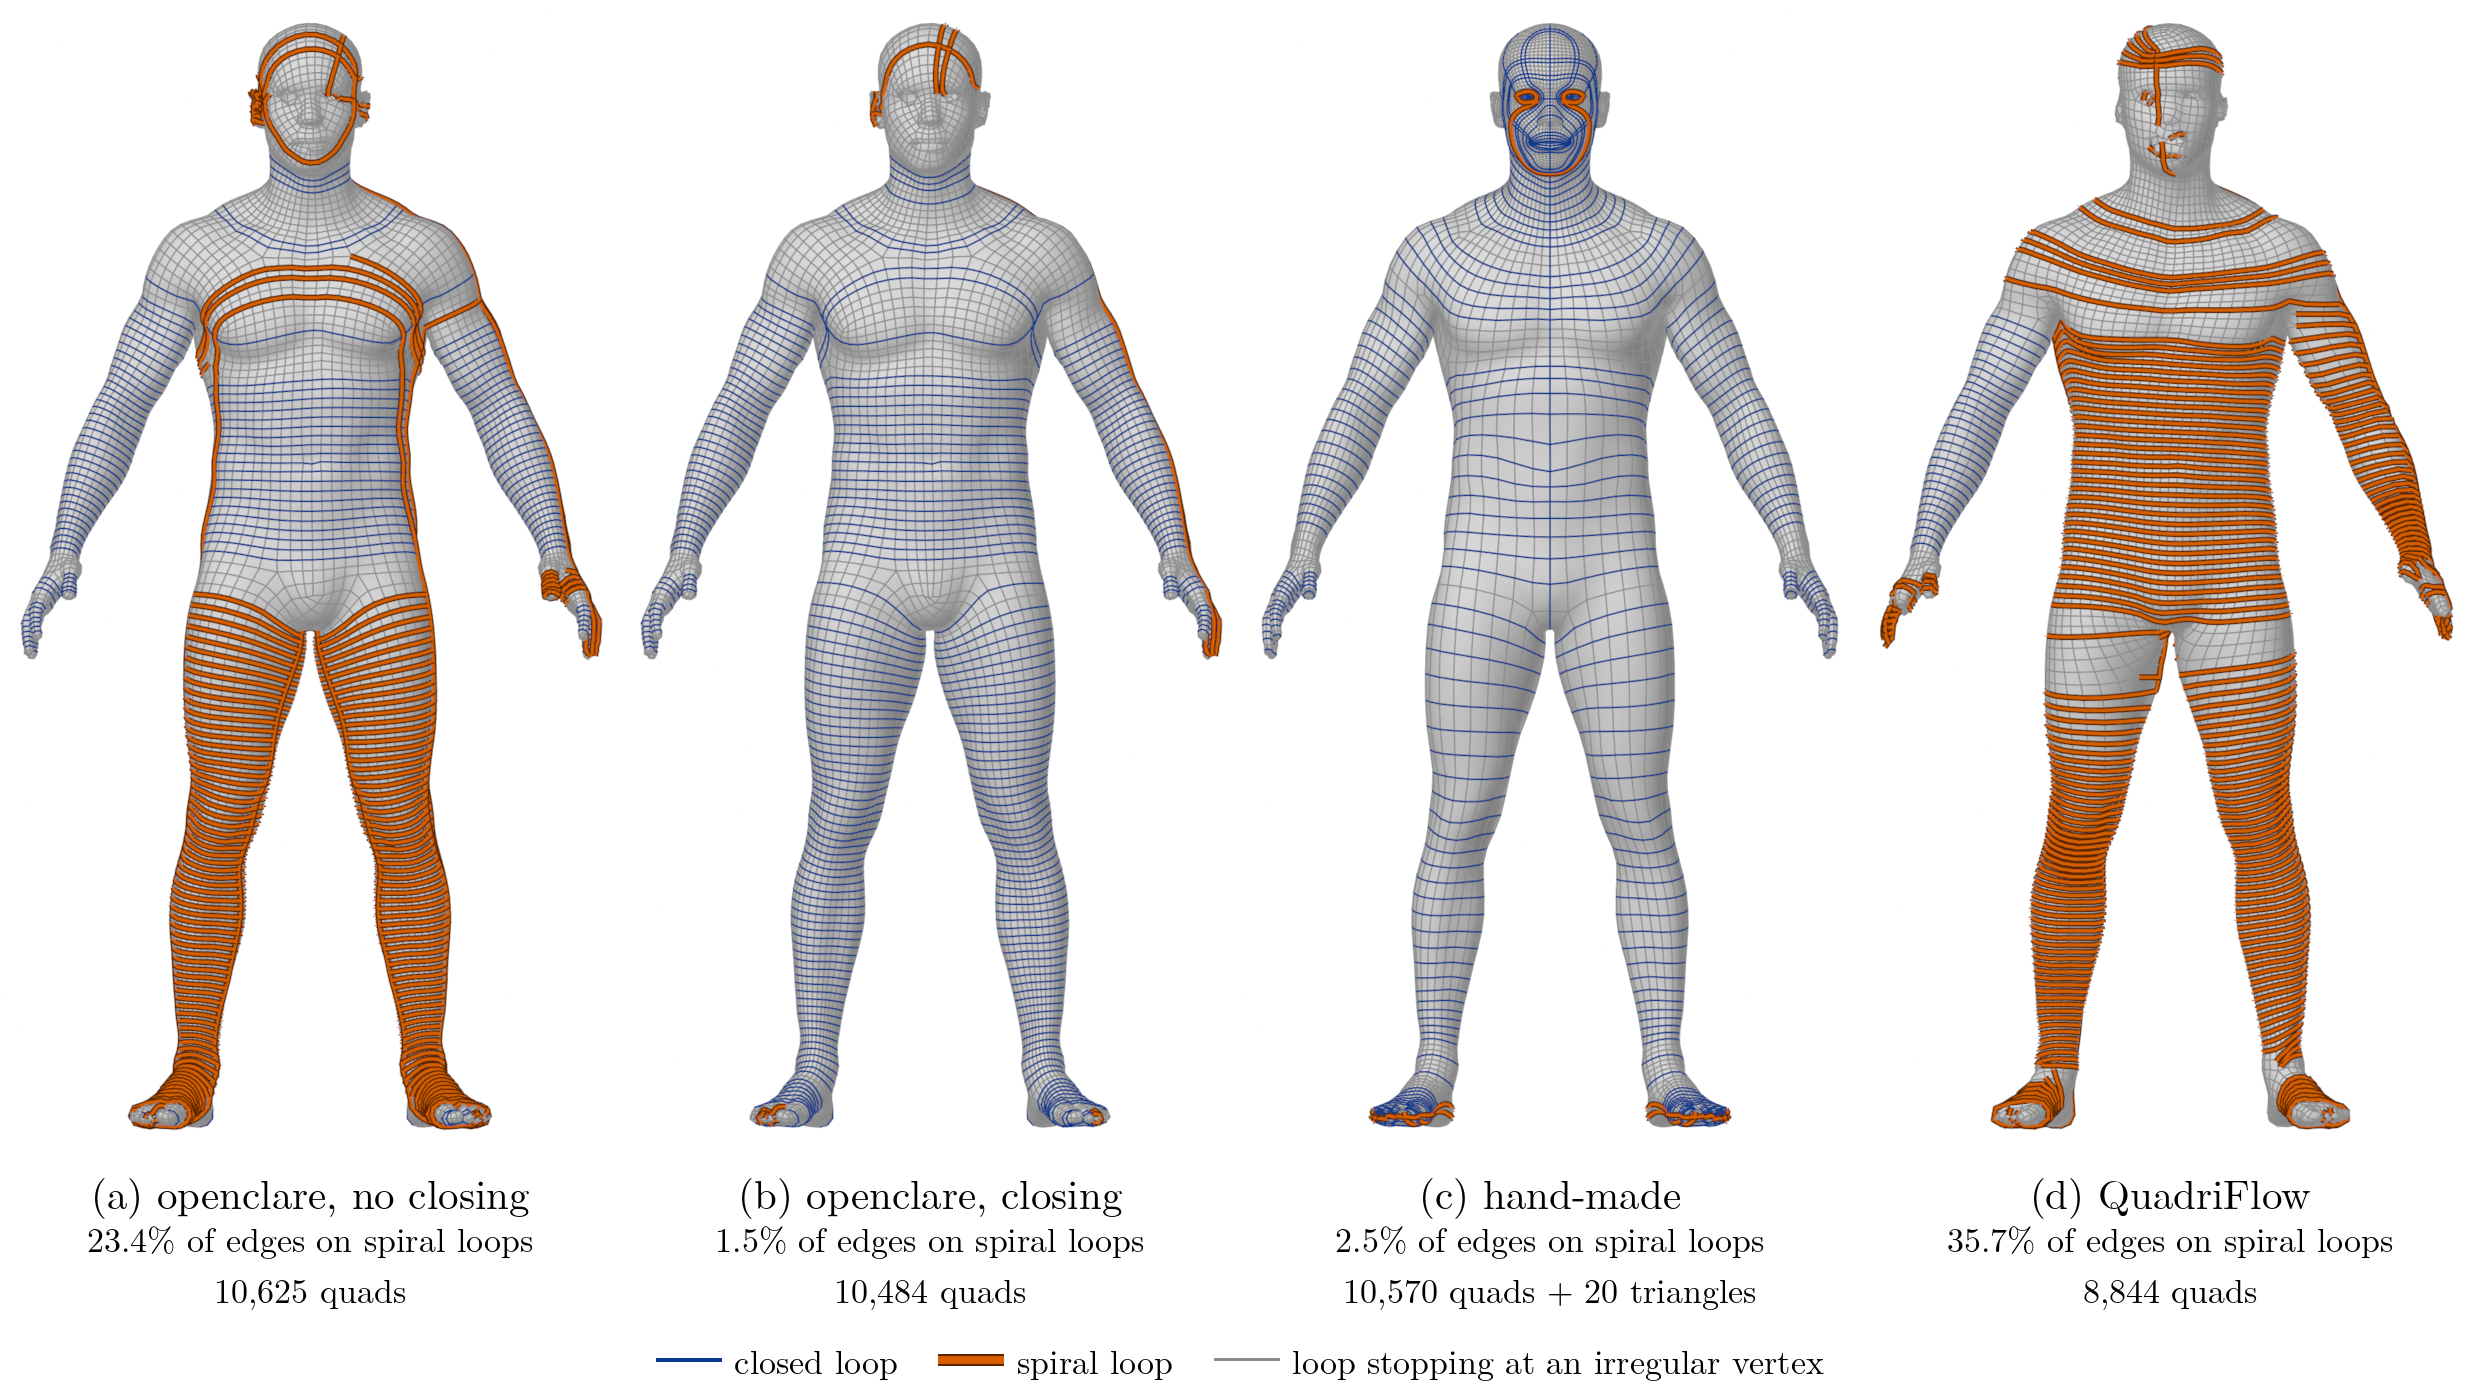
\includegraphics[width=\textwidth]{figures/male-overview.png}
\caption{The male body of the Essentials library, $10{,}590$ quads asked
for: (a)~openclare without closing, (b)~openclare with the closing of
Section~\ref{sec:closing}, (c)~the base mesh modelled by hand,
(d)~QuadriFlow run through Blender, on the source scaled by $100$ and scaled
back: Blender refuses the sculpt as it is, some of its edges being shorter
than its threshold of $10^{-4}$, and QuadriFlow does not depend on the scale.
Edge loops are coloured by their kind in
the measure of Section~\ref{sec:measure}: closed loops dark blue, spiral
loops vermillion (wider, with a dark rim), loops that stop at an irregular
vertex grey. Meshes (a) and (b) come from the engine of version 0.7.0, one
deterministic run each, the runs quoted in the text. Measured on the whole
meshes, they have $10{,}625$, $10{,}484$, $10{,}570$ (plus $20$ triangles)
and $8{,}844$ quads, $23.4\%$ ($21$ loops), $1.46\%$ ($11$), $2.55\%$ ($3$)
and $35.7\%$ ($43$) of their edges on spiral loops, which the panels round to
one decimal, and $17.2\%$, $36.5\%$, $31.6\%$ and $2.7\%$ on closed loops.
QuadriFlow's mesh has $3$ inverted faces and a Hausdorff distance of
$31$\textperthousand\ of the diagonal.}
\label{fig:overview}
\end{figure*}

\begin{figure*}[t]
\centering
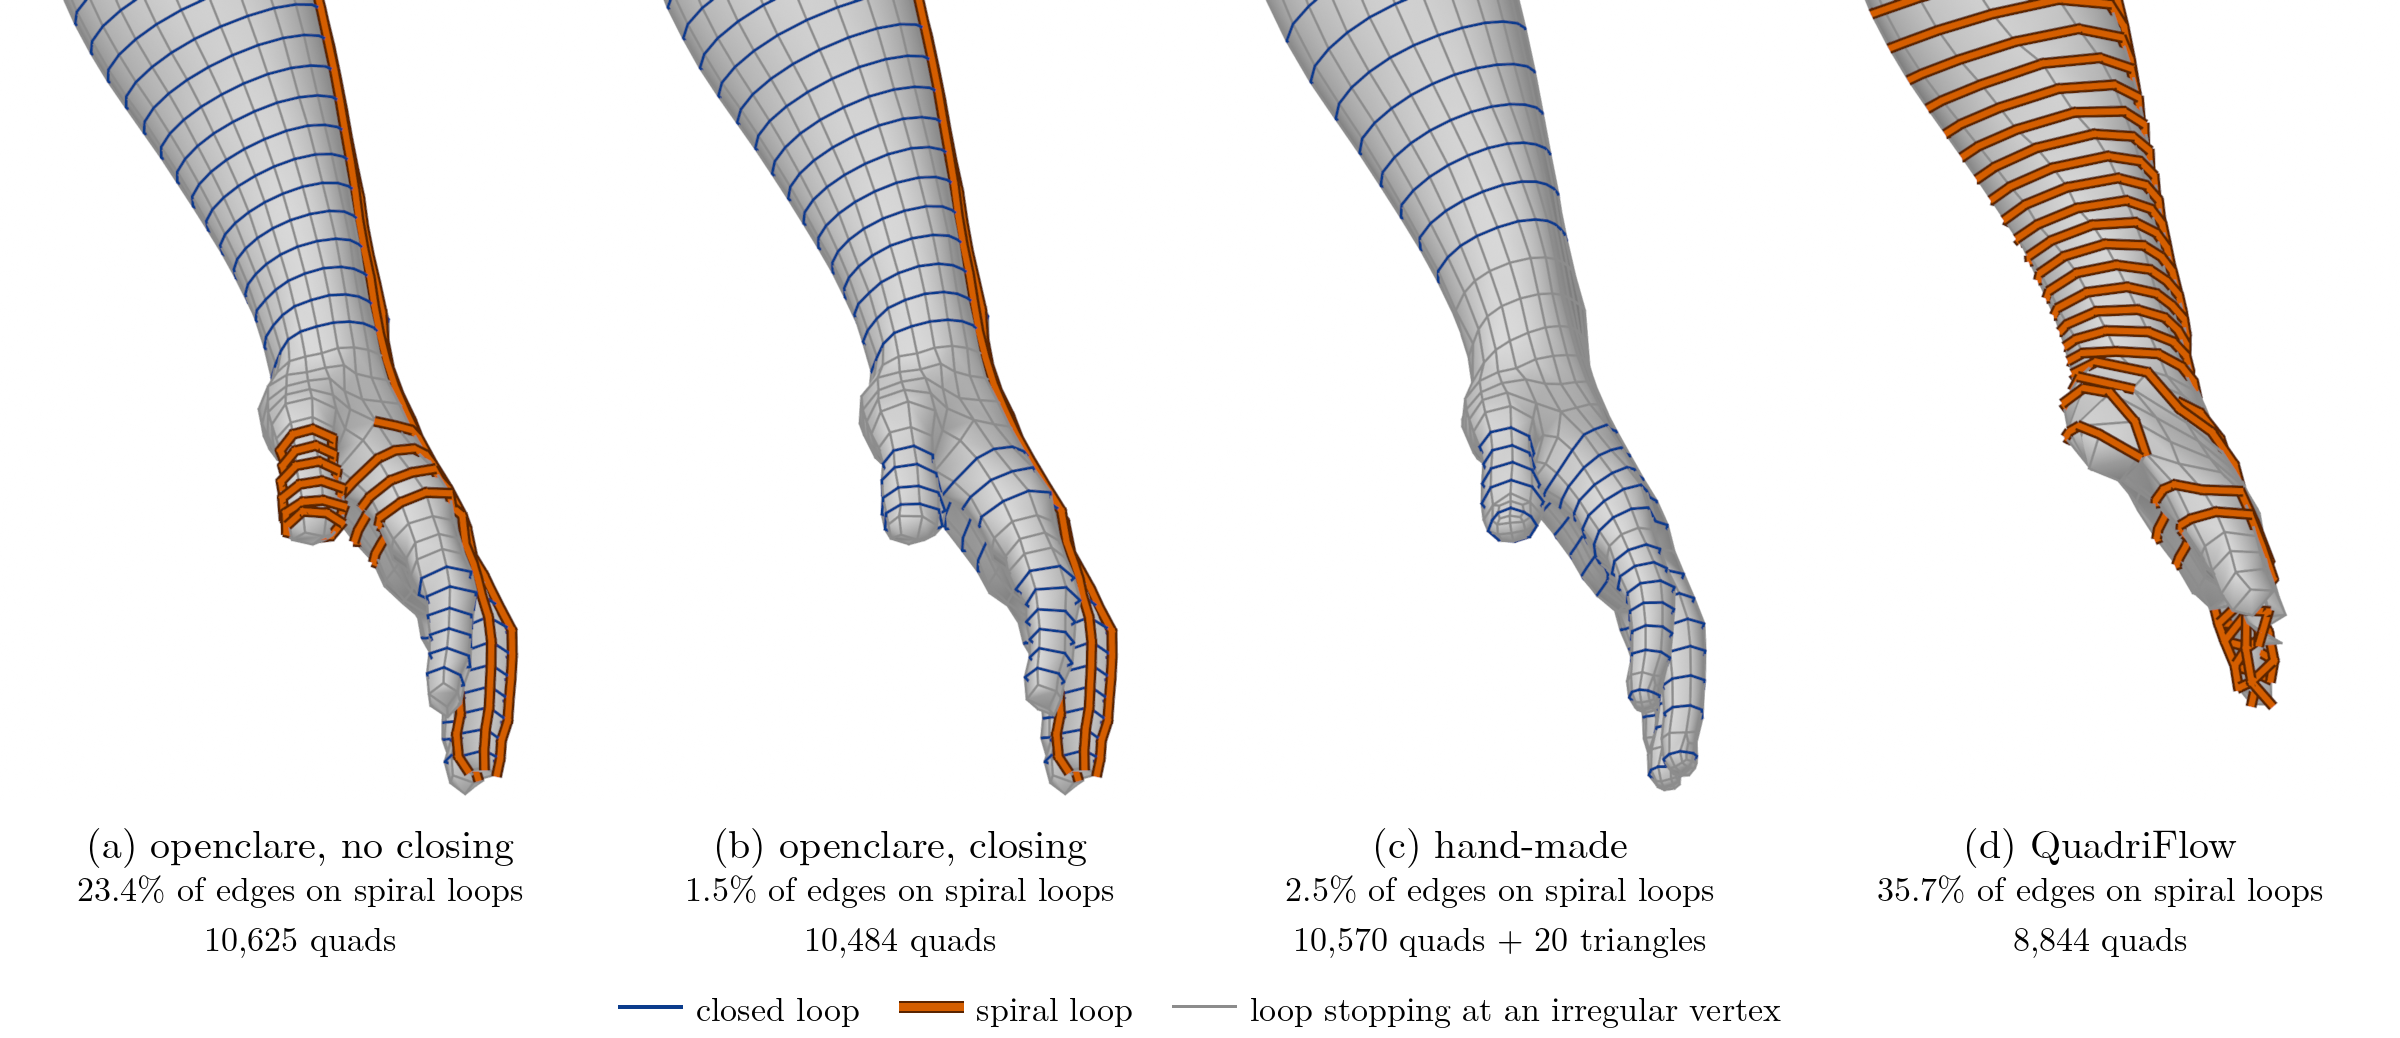
\includegraphics[width=\textwidth]{figures/male-wrist.png}\\[0.6em]
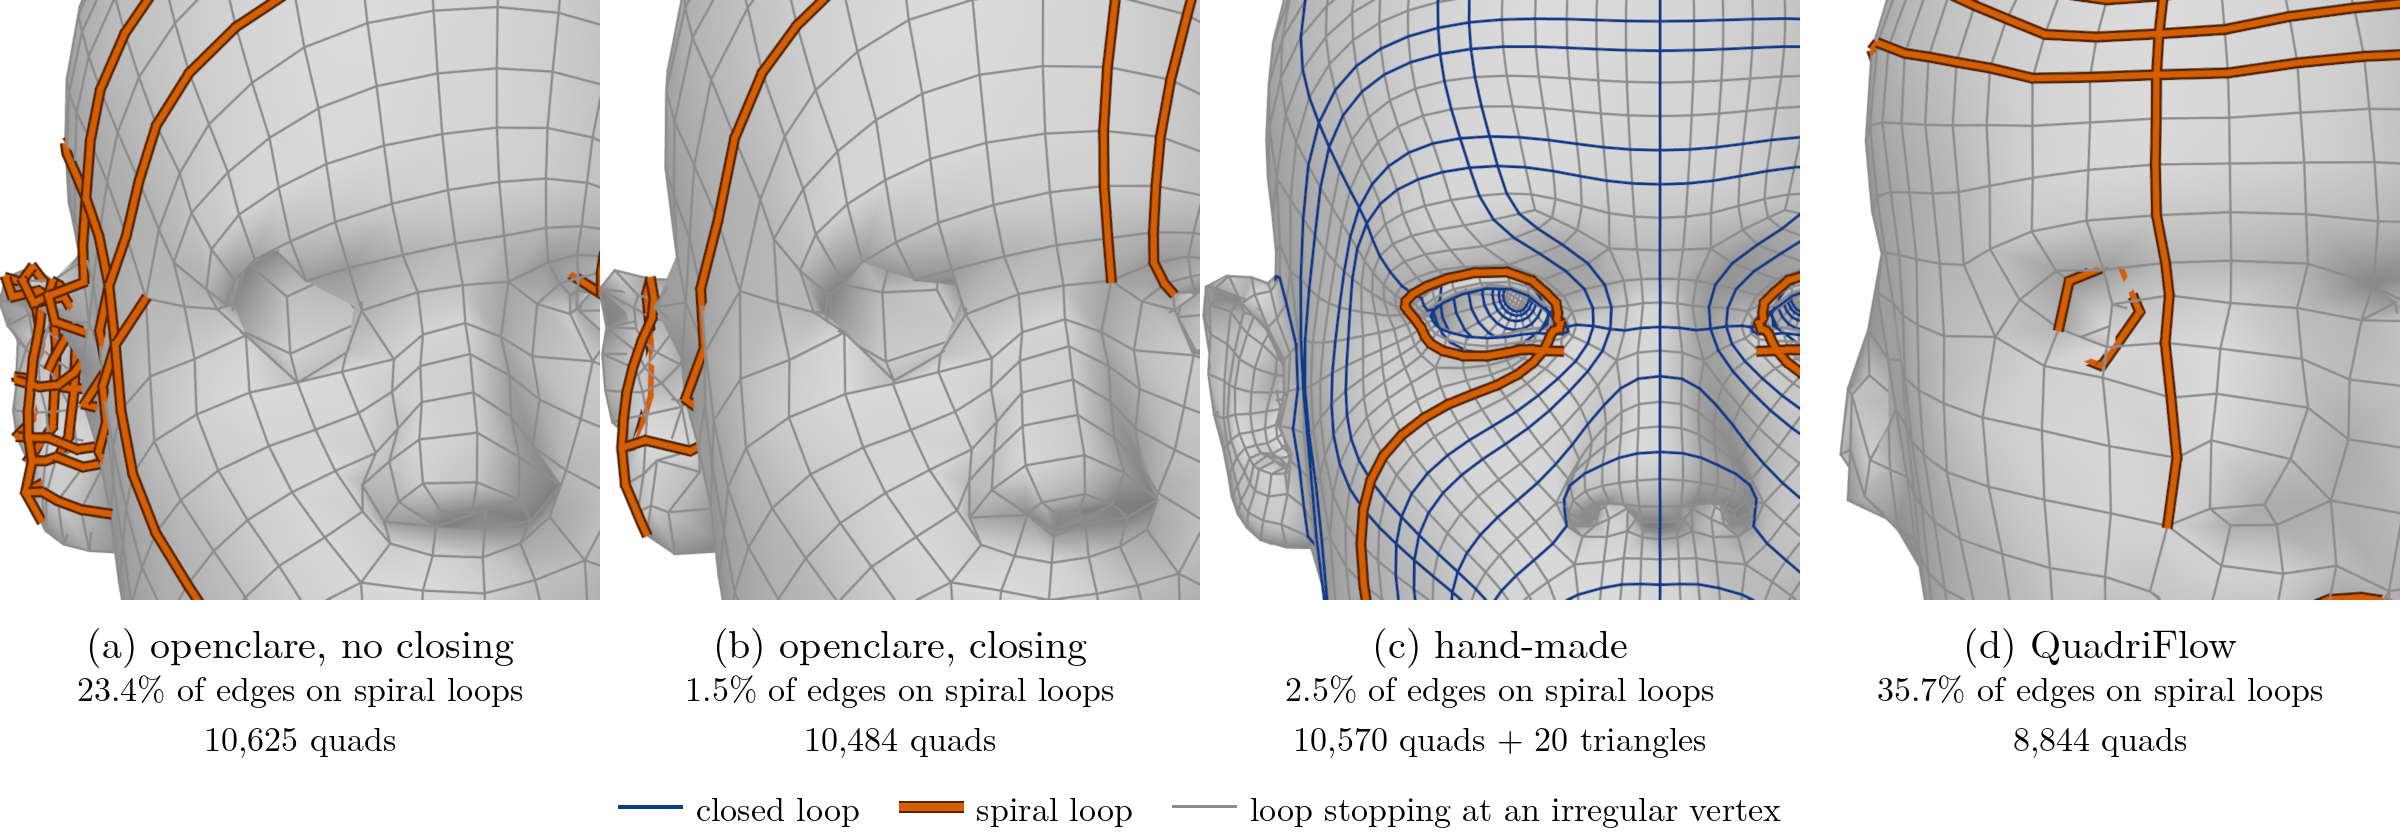
\includegraphics[width=\textwidth]{figures/male-eye.png}
\caption{Close-ups of the four meshes of Figure~\ref{fig:overview}, in the
same order and colours: the left wrist and hand (top; the body's left, on
the viewer's right in Figure~\ref{fig:overview}) and the right eye
(bottom). At the wrist, mesh~(b) has closed loops on the thumb and the back
of the hand where mesh~(a) has spiral ones, and a spiral loop along the outer
side of the forearm remains on both. At the eye, neither openclare mesh has
a spiral loop near the eye, both keep spiral loops on the forehead and at the
ear, and the loop round the eye of the hand-made mesh is itself counted as
spiral.}
\label{fig:closeups}
\end{figure*}

\section{An exact look at the closing system}\label{sec:exact}

How far is the heuristic of Section~\ref{sec:closing} from what the
constraints allow? An experiment option of the engine exports, for each way
of finding turns, the system it works on; we export it for the male body at
$10{,}590$ quads, from the engine as it runs. Its T-mesh has $1{,}342$ nodes
($1{,}068$ T-junctions, $254$ singular vertices, $131$ of valence three and
$123$ of valence five, and $20$ corners of folds), $2{,}146$ arcs and $806$
patches, hence $1{,}612$ balance equations, one per patch and direction. The
export gives the real lengths, every turn found with its shift (on all
$1{,}708$ turns, composing the crossing maps along the walk gives the
exported shift), and the lower bounds the integer search placed on arcs to
keep singularities apart ($36$ to $197$ arcs held at length one, depending on
the way). These bounds are the engine's choice of
\emph{which} arc of a chain between two singular vertices carries their
separation: validity asks a chain to keep a positive total length, not a
given arc. Every statement below is relative to them. We call
$P_{\mathrm{eng}}$ the balanced lengths that meet them; it is neither a
subset nor a superset of the valid quantizations, since it excludes valid
lengths that put the separation on another arc of the chain and allows
lengths that bring other arcs to zero. The ways are numbered as exported:
way $m + 2j + 4i$ starts from the shares $\{0.5\}$ ($m = 0$) or $\{0.2, 0.5,
0.8\}$ ($m = 1$), with the lean bound $0.05$ ($j = 0$) or $0.12$ ($j = 1$)
and the length bound $2$ ($i = 0$) or $6$ ($i = 1$) sides. Without the
other draws the engine keeps way~2 for this body ($1.65\%$ of spiral edges);
with them it keeps the lengths of another draw ($1.46\%$).

\paragraph{The conflict is real but local.}
All held turns can be closed together if the lengths are only asked to be
non-negative; with the bounds of separation, they cannot. By Farkas' lemma a
set of turns cannot be closed within the bounds exactly when some
combination of their shifts equals, modulo the balances, a non-negative
combination of arc lengths that charges an arc held open, and the companion
paper~\cite{gardent2026turns} reads these certificates on the singularities.
In seven ways (all but way~4) some held turn cannot even be closed on its
own. In five of them (0, 1, 2, 5 and 7) it is the same turn, of length
$6.76$, whose shift equals, modulo the balances, $-(\ell_{1892} +
\ell_{1908})$, where arc $1908$, less than $0.09$ quad edges long in the
parametrization, is held at length at least one; in ways 2, 3, 6 and 7 a
second turn, of length $4.72$, is held up in the same way by arc~$1006$ (both
certificates checked in exact rational arithmetic).
Whether $\ell_{1908} = 0$ would merge two singular vertices, that is whether
every valid quantization meets this bound, we did not check. Giving up the
least total amount of the bounds needed to close all held turns, a linear
program, shows that in way~0 the bound of arc $1908$ alone stands in the
way, in way~2 three bounds, that one among them, and in the other ways $6$
to $154$.

\paragraph{How many held turns can close.}
With every bound kept, the largest set of held turns that can be closed
together is found by a mixed-integer program with one binary per turn
(Table~\ref{tab:exact}). The projection of the engine keeps every held turn
closed: its active set asks the lengths to be non-negative only, which, as
above, lets all held turns close; the bounds of separation return in the
integer search. In whole numbers, the same mixed-integer program, with a
limit of fifteen minutes a way, proves its optimum in way~3 only ($90$
turns, as in real numbers); in the other ways it stops with $1$ to $88$
turns fewer than in real numbers.

\begin{table}[t]
\centering
\begin{tabular}{lrr}
\toprule
way & held & closable together \\
\midrule
0 & 58 & 57 \\
1 & 92 & 87 \\
2 & 64 & 61 \\
3 & 102 & 90 \\
4 & 125 & 120 \\
5 & 219 & 189 \\
6 & 131 & 123 \\
7 & 229 & 192 \\
\bottomrule
\end{tabular}
\caption{Male body at $10{,}590$ quads, real numbers, engine of version
0.7.0. ``Closable together'': the largest set of held turns closable with
every bound of separation kept; in way~7 the program stopped at its limit
of $300$ seconds, with a bound of $195$.}
\label{tab:exact}
\end{table}

\paragraph{The rounding ignores the shifts.}
Feeding the integer search of the engine better targets shows what survives
it (Table~\ref{tab:rounding}). The active-set projection, the engine's,
keeps every held turn closed in real numbers, yet after the integer search
$33\%$ to $74\%$ of them are shifted again ($170$ of $229$ in way~7); with a
least-squares projection whose negative lengths are clamped to zero, too,
about $40\%$ of the turns it closes are shifted after the integer search.
The integer search follows the targets but not the shifts. Aiming at the
lengths of the linear program, whose weighted $L^1$ objective puts the
changes on few arcs, the engine ranks first a candidate with $2.63\%$ of
spiral edges, yet outputs the mesh of the plain lengths: after meshing, the
candidates ranked before them were set aside.

\begin{table}[t]
\centering
\small
\begin{tabular}{lrrr}
\toprule
targets of the integer search & turns closed in reals & still shifted after & spiral edges (mesh) \\
\midrule
projection, clamped & 41--52 & 15--25 of them & 2.11\% \\
linear program, $L^1$ & 57--192 & 14--133 of them & 23.39\% \\
active set, floor 0 (the engine) & all held (58--229) & 19--170 of them & 1.46\% \\
active set, floor half the real length & 51--132 & 19--93 of them & 2.80\% \\
\bottomrule
\end{tabular}
\caption{Male body at $10{,}590$ quads, engine of version 0.7.0 with its
experiment options, one run each; ranges over the eight ways. The mesh keeps
the candidate with the fewest spirals, so its share is that of a single way
or draw; with the linear program it is the mesh of the plain lengths.}
\label{tab:rounding}
\end{table}

\paragraph{Whole lengths are not what is missing.}
The balances are the incidence matrix of a bidirected graph whose nodes are
the balance equations and whose edges are the arcs (each arc lies on a side
of each of the two patches it borders). When this graph is connected and has
a cycle that $\pm1$ values cannot balance, as on the body, the companion
paper shows that a set of free arcs parametrizes the lattice of whole
balanced lengths: here $2{,}146 - 1{,}612 = 534$ arcs can be given any whole
lengths and the others follow, so balances alone never obstruct whole
lengths. Closing exactly, in whole numbers, the turns found closable
together, HiGHS finds such lengths in $83$ to $228$ seconds in ways 0 to 3,
and none within ten minutes in ways 4 to 7. The solutions leave $1$, $5$,
$3$ and $12$ held turns shifted where the engine leaves $19$, $40$, $23$ and
$52$, and fewer of the turns not held as well ($3$ against $15$, $9$ against
$25$, $5$ against $18$, $11$ against $34$), at a weighted deviation from the
real lengths $2\%$ to $64\%$ higher. Yet three of the four spiral
\emph{more}, by the engine's count on the connectivity of their lengths:
$5.9\%$, $2.8\%$ and $7.8\%$ of their edges against $4.1\%$, $1.7\%$ and
$3.5\%$ for the engine's lengths in ways 0, 2 and 3; in way~1, $4.9\%$
against $9.1\%$. Only those of way~2 stay within the engine's window of
sizes; the others have $10{,}857$, $12{,}420$ and $11{,}011$ quads. Most of
the loops that spiral are not turns the sampled walks find.

Walking every strip of the mesh of way~2 instead
(Proposition~\ref{prop:complete}) finds $306$ ways round, each strip twice,
once in each direction; $236$ come back shifted. Selecting them by lean, as
the constraint rounds do, keeps $298$, of which $270$ ($135$ strips) can be
closed together in real numbers with every bound kept. Posed directly to
HiGHS, they gave no whole solution in $12{,}651$ seconds; given the $341$
arcs that every real solution sets to zero (each certified by a non-negative
combination of shifts, $216$ certificates over $36$ distinct sets of rings),
none was found in $2{,}596$ seconds either. No real lengths closing the
$270$ rings have a mean deviation from the targets below $1.304$, where the
engine allows $0.522$ ($0.2$ above the $0.322$ of its plain search). The
largest subset closable within a mean deviation of $0.4$, the number of
quads held to first order, found by a program stopped after $600$ seconds,
has $228$ rings (at most $267$) and closes at $0.395$ in real numbers. In
whole numbers, with the reformulation of Aardal, Hurkens and
Lenstra~\cite{aardal2000diophantine} on an LLL-reduced
basis~\cite{lenstra1982lll} of the lattice of closed quantizations, HiGHS,
stopped after $1{,}200$ seconds, finds whole lengths closing all $228$
within every bound at a mean deviation of $0.535$ and $10{,}653$ quads, and
proves that none does better than $0.518$. These lengths lie above the
engine's cap ($0.535$ against $0.522$), so the engine does not take them as
a candidate. Rounding costs between $0.123$ (proven) and $0.140$ (found) of
mean deviation above the real optimum.

\paragraph{The heuristic leaves most of the gap.}
The companion paper~\cite{gardent2026turns} computes the least number of
held turns that any lengths in $P_{\mathrm{eng}}$ leave shifted, a minimum
cover of the irreducible infeasible subsystems~\cite{parker1996iis}: exactly
$1$, $5$, $3$, $12$, $5$, $30$, $8$ and $37$ in ways 0 to 7, against $19$,
$40$, $23$, $52$, $61$, $154$, $72$ and $170$ left shifted by the engine.
With the engine's cap on the deviation and its window of sizes ($10{,}379$
to $10{,}801$ quads) added, at whole lengths, the least number is still
exactly one in way~0 and three in way~2: whole lengths closing every other
held turn exist at $10{,}730$ and $10{,}435$ quads, at mean deviations
$0.387$ and $0.506$. Of the $23$ turns of way~2 the engine leaves shifted,
the bounds of separation force three and the cap, the size and integrality
none; the heuristic accounts for $20$. Closing more turns, however, is not
what the measure of spirals sees: a local search over whole lengths within
the same cap and size closes $45$ more strips of the mesh of way~2 than the
engine does, but at its lengths, where the strips are other walks, $4.7\%$
of the edges spiral, against $1.7\%$ at the engine's lengths of way~2; it is
the choice of the turns to close, at the lengths where they are the strips
of the mesh, that decides how much the mesh spirals. Choosing the most turns to close
is NP-hard for bidirected balances with $0$--$1$ bounds, the algebraic form
of quantization~\cite{gardent2026turns}; whether the balances and turns of an
actual T-mesh stay hard is open.

\paragraph{Closing the most rings, end to end.}
We measured what an exact selection buys on the bench with the slow quality
mode of the engine (\texttt{--quality slow}), against the engine without its
other draws ($5.85\%$ of spiral edges over the $36$ runs), with three
($5.43\%$) and with its twelve ($4.92\%$). For the lengths the engine keeps,
a mixed-integer program closes as many of its strips leaning less than
$0.12$ as it can, weighted by their length round, within the balances, the
bounds of separation, the cap and the quad budget. A strip counts as closed
only where the corridor inequalities~\eqref{eq:corridor} hold for it, so
that it keeps its walk at the new lengths. The engine meshes the result, the
strips are walked again at the new lengths, and the program solved again,
three rounds; each round's lengths join the engine's candidates on the same
terms. The program is solved by HiGHS linked into the engine, each solve
stopped at a work limit (simplex iterations times arcs) that does not depend
on the load. Without the other draws, the slow mode lowers the mean to
$4.41\%$: lower on $9$ of the $36$ runs, never higher. Closed loops ($36.6\%$
against $35.4\%$ of the edges) and mean distance ($0.382$\textperthousand\
in both) barely move, and all $36$ meshes are valid. Against the twelve
other draws it is lower on average ($4.41\%$ against $4.92\%$) but not run
by run: higher on $9$ runs, lower on $5$. On the male body its three rounds
return the lengths they start from: $1.65\%$, as without it, against
$1.46\%$ for the engine with its draws. The gain does not need a solver that
finishes: $90$ of the $120$ solves stop at the work limit, and with a limit
of $5$ seconds per solve instead, $76$ of $100$ stop at it, $18$ of the $66$
rounds (against $12$) return the lengths they start from, and the mean is
$4.56\%$, on four processors where the other runs had eight.

\paragraph{Acting before quantization.}
Moving singular vertices in the parametrization, and rotating the field
cylinder by cylinder, were also tried, with prototypes of the engine that are
not part of it; neither lowered the share of spirals. The Burgers sum of the
companion paper~\cite{gardent2026turns} accounts for it: the shifts of two
parallel turns differ by the across component of the Burgers vector of the
singular vertices between them, which depends only on their developed
positions, so closing one turn by a local change of the map moves its shift
onto the turns beside it. The conflicts are better attacked in quantization.

\section{Limitations and open problems}\label{sec:limits}

The results come from one implementation and are preliminary. The spiral
share of a single model is chaotic, so only the means over three budgets are
robust; the other figures are single runs. The measure sees helices of pitch
up to four only. The exact look covers one body and holds relative to the
engine's bounds of separation, which are its choice of arcs and neither a
subset nor a superset of the valid quantizations. The machine was shared:
its load is recorded, not controlled, and the outcomes that depend on a
time limit depend on it.

Three problems remain open. \emph{An exact formulation}: minimizing the
deviation subject to the balances, the bounds and $\shift_\gamma(\ell) = 0$
for a set of turns is a minimum-deviation flow with linear side constraints;
how much of the exact machinery of~\cite{heistermann2023bimdf} carries over is
open, and the linear relaxation already closes $84\%$ to $98\%$ of the held
turns.
\emph{Closing in whole numbers}: whole lengths closing every ring asked for
are found through a reduced lattice basis, but in minutes, with the number
of quads held only to first order and $0.12$ to $0.14$ above the real optimum
in deviation, here above the engine's cap; can the integer search move within this lattice at the speed of
a flow solver? \emph{Which turns}, the central one on the evidence of
Section~\ref{sec:exact}: closing rings changes the lengths, the lengths
change the strips, and the strips of the new mesh are other walks. Is there a
finite set of turns whose closing implies that every loop of the quad mesh
closes? Can the loops of the quad mesh be read off the T-mesh and its lengths
directly, so that every one is accounted for? Which objective, short of all
loops, predicts the spirals the measure sees?

\section*{AI assistance}
This note and the software it describes were made by a human author working
with an AI system, which is not an author. The author chose the problem and
its aims (edge loops that close into rings and, as an artist, few singular
vertices and few spirals rather than perfectly square quads, quads only), set
the direction and the order of the work, decided which results to pursue and
which changes to merge, and judged the results through the measurements,
pictures and drafts presented to him. Claude Opus 5.5 (Anthropic), used
through Claude Code in October 2026 with several sub-agents in parallel,
wrote the changes to the engine and the experiment scripts, ran all the
experiments and exact computations, searched the literature, stated and
proved the propositions, and drafted the text. References were checked for
existence, and the note of each bibliography entry says how much of the work
was read. A work of which only the abstract, or a review, was read is cited only for what that abstract or review states. Weaker forms of Propositions~\ref{prop:linear}
and~\ref{prop:complete} are checked in Lean~4~\cite{demoura2021lean4} in the
companion paper, as the tag above each says; everything else here not checked by machine was written
with AI help and checked by AI agents rereading it and testing it on the
data, not by a human expert. The note has not been peer reviewed; the author,
who publishes it, is responsible for its content.

\bibliographystyle{plainnat}
\bibliography{refs}

\appendix

\section{Provenance of the figures}\label{app:provenance}

Every figure comes from the engine of version 0.7.0 (commit
\texttt{e13fadb}), built in release mode, and from the scripts of
\nolinkurl{docs/research/closing-loops/experiments/} (those of
Section~\ref{sec:exact} in its folder \nolinkurl{exact/}) and, for the
census, the conflicts and the least number of turns left shifted, which the
companion paper shares, of \nolinkurl{docs/research/turns-of-a-t-mesh/experiments/}.
Each script writes a summary, \texttt{results/}\textit{name}\texttt{.json}
beside it, with the engine's commit and build, the machine, its load and the
solver's version; its README gives the command of every table. The raw
output (meshes, exports, logs) is not in the repository.

\begin{center}
\small
\setlength{\tabcolsep}{4pt}
\begin{tabular}{@{}>{\raggedright\arraybackslash}p{5.6cm}>{\raggedright\arraybackslash}p{4.6cm}>{\raggedright\arraybackslash}p{4.4cm}@{}}
\toprule
figures & script & summary \\
\midrule
twelve models, three budgets (Section~\ref{sec:experiments})
  & \texttt{twelve\_models.py}, the protocol below
  & \texttt{twelve\_models.json} \\
Table~\ref{tab:dev}
  & \texttt{ablation.py}; its last line gave the $36$ meshes above byte for
  byte
  & \texttt{ablation.json} \\
against other remeshers
  & \texttt{against\_remeshers.py}, from \nolinkurl{bench/results/results.json}
  at \texttt{e13fadb}
  & \texttt{against\_remeshers.json} \\
male body, openclare and hand-made
  & \texttt{male\_body.py}
  & \texttt{male\_body.json} \\
Figures~\ref{fig:overview} and~\ref{fig:closeups}, their numbers
  & \texttt{figures/make\_figures.sh}, \texttt{figure\_numbers.py};
  QuadriFlow through Blender, on the source scaled by $100$ and scaled back
  & \texttt{figures.json} \\
Section~\ref{sec:exact}: the T-mesh, the conflicts, the least numbers left
shifted
  & \texttt{census.py}, \texttt{holonomy.py}, \texttt{conflicts.py},
  \texttt{forced.py} of the companion paper
  & their summaries of the same names \\
Section~\ref{sec:exact}: the other figures and Tables~\ref{tab:exact}
and~\ref{tab:rounding}
  & \texttt{exact/}: \texttt{relaxation.py}, \texttt{most\_closable.py},
  \texttt{rings.py}, \texttt{lattice\_rounding.py}, \texttt{local\_search.py},
  \texttt{remesh.py}
  & their summaries of the same names \\
closing the most rings, end to end
  & \texttt{exact/end\_to\_end.py}
  & \texttt{end\_to\_end.json}; the limit of $5$ seconds:
  \texttt{end\_to\_end-time-5.json} \\
\bottomrule
\end{tabular}
\end{center}

\paragraph{The protocol of the twelve models.} For each model $m$ (creature,
blob, suzanne, spot, pig, ogre, bob, jerry, blub, rock with the preset
\texttt{organic}; cage and part with \texttt{hard-surface}) and each budget
$Q \in \{2{,}970, 3{,}000, 3{,}030\}$: \texttt{openclare remesh}
\texttt{bench/out/}$m$\texttt{/source.obj} \textit{out.obj}
\texttt{--preset} $P$ \texttt{--quads} $Q$, then \texttt{openclare measure}
on the source and the output with \texttt{--target} $Q$ \texttt{--json}; the
figures are the means of \texttt{loop\_edges\_spiral},
\texttt{loop\_edges\_closed}, \texttt{loops\_spiral},
\texttt{mean\_distance} and \texttt{angle\_deviation\_mean} over the $36$
runs.

\paragraph{Reproducibility.} The method is implemented in openclare (Rust),
in the main branch of the repository; the bench is driven by
\texttt{bench/run.py}. The export of the T-mesh and the switches of
Table~\ref{tab:dev} are experiment options of the engine of version 0.7.0
(\texttt{ALGORITHM.md}, ``Experiment options''), and the slow quality mode
is its option \texttt{--quality slow}, so the scripts above make every
figure again on that engine; the figures that
depend on a time limit depend on the machine and its load as well. The
prototypes of ``Acting before quantization'' are not part of the engine and
are not scripted. This version of the note was built from commit
\texttt{\enginecommit}.

\end{document}
 gives the paper
% without them, for a venue that wants it plain.
\newcommand{\lean}[1]{\texttt{\detokenize{#1}}}
\ifdefined\plain
\newenvironment{evidence}[3][]{}{}
\else
\usepackage[most]{tcolorbox}
\newcommand{\evlevel}[2]{\expandafter\newcommand\csname ev-name-#1\endcsname{#2}}
\evlevel{lean}{Lean, complete}
\evlevel{core}{Lean, algebraic core}
\evlevel{data}{Checked on the engine's data}
\evlevel{measured}{Measured}
\evlevel{prose}{Proof on paper only}
\evlevel{tested}{Conjecture, checked by computer}
\evlevel{cited}{Standard, cited}
\evlevel{open}{Open, no claim}
\newcommand{\evname}[1]{\csname ev-name-#1\endcsname}
\tcbset{evstyle-lean/.style={}, evstyle-core/.style={}, evstyle-data/.style={},
  evstyle-measured/.style={}, evstyle-tested/.style={}, evstyle-prose/.style={},
  evstyle-cited/.style={},
  evstyle-open/.style={frame hidden, borderline={0.4pt}{0pt}{black!45, dashed}}}
\newtcolorbox{evidence}[3][]{breakable, enhanced, colback=white,
  colframe=black!45, boxrule=0.4pt, arc=0pt, left=4pt, right=4pt, top=2pt,
  bottom=2pt, before skip=6pt, after skip=6pt, evstyle-#2,
  title={\footnotesize\textsc{\evname{#2}}\if\relax\detokenize{#3}\relax\else
    \quad #3\fi},
  coltitle=black, colbacktitle=white, titlerule=0.4pt, toptitle=1pt,
  bottomtitle=1pt, #1}
\fi

\title{Closing Edge Loops at Quantization Time:\\
Helix Constraints for T-Mesh Quantization\\[0.5em]
\large Research note --- draft, not peer reviewed}
\author{Marc Gardent%
\thanks{This note is distributed under the Creative Commons Attribution
4.0 International licence (CC BY 4.0). The code of openclare is under the
GPL-3.0-or-later of the repository. The note describes the engine at commit
\texttt{\enginecommit} of \url{https://github.com/marcgardent/openclare}.
A French translation is in \texttt{paper.fr.pdf}, beside this note.}\\
\normalsize Independent researcher\\
\normalsize ORCID: \href{https://orcid.org/0009-0000-6466-3098}{0009-0000-6466-3098}\\
\normalsize Contact: through the repository,
\url{https://github.com/marcgardent/openclare}}
\date{October 2026}

\begin{document}
\maketitle

\begin{abstract}
Automatic quad remeshing often produces edge loops that wind round a part of
the shape as helices instead of closing into rings. Bommes et
al.~\cite{bommes2011structure} remove such \emph{q-helices} from a finished
mesh; we prevent them where the integer structure of the mesh is decided, in
the quantization of a T-mesh. A straight walk across the patches of a T-mesh
that returns to its first side, a \emph{turn}, has a \emph{shift} that is an
integer linear form in the arc lengths; at whole lengths it is how far the
strip of quads following the turn comes back beside itself, and every strip
of the mesh is such a walk. We add the constraints that close turns to a
minimum-deviation quantizer~\cite{heistermann2023bimdf}, through a
least-change projection, repair walks and rounds of constraint generation on
the strips of the mesh, and keep the candidate with the fewest spiral edges,
counted by a test that tells helices from closed, open and border loops. Over
twelve models at three budgets near 3{,}000 quads, the engine leaves 4.92\%
of the edges on spiral loops (19.8\% without closing); on the seven models
that two other open-source remeshers also mesh validly, 2.2\% against 38.8\% % NIGHT4
and 21.7\%; on a human body, 1.5\%, against 2.5\% for the hand-made mesh.
An exact analysis of the closing system of that body shows that the conflict between closing
turns and keeping singularities apart is real but local, that the heuristic
rather than the constraints leaves most turns shifted, and that closing more
turns does not by itself make fewer spirals: the strips move with the
lengths, and the choice of the turns to close decides.
\end{abstract}

\section{Introduction}

In our experience, element shape and alignment are rarely what limits
field-aligned quad remeshing today (see the
surveys~\cite{bommes2013survey,campen2017survey}). What remains is structure:
the way edge loops run across the surface. Artists expect a loop round an
arm, a leg or a neck to be a ring. Automatic methods often produce a helix
instead: the loop goes round, comes back one or a few rows further, and winds
along the whole part (Figure~\ref{fig:overview}). Bommes et al.\ showed that
helical configurations are a main reason why the base complex of an otherwise
good quad mesh stays dense~\cite{bommes2011structure}, and removed them from
the finished mesh.

Whether a loop closes is decided upstream, when a quantizer assigns whole
lengths to the arcs of a T-mesh traced in a seamless
parametrization~\cite{campen2015qgp,lyon2021constrained,heistermann2023bimdf}.
Quantizers choose these lengths for consistency, validity and closeness to
the parametrization; the loops close or spiral as a side effect. This paper
constrains the loops in the quantization itself. Section~\ref{sec:turns}
defines \emph{turns}, straight walks across the patches of a T-mesh that
return to their first side, and shows that the \emph{shift} of a turn is an
integer linear form in the arc lengths that gives, at whole lengths, the
pitch of the strip of quads following it, and that every strip of the mesh
is such a walk. Section~\ref{sec:closing} adds the closing of turns to a
minimum-deviation quantizer through a least-change projection, repair walks
and rounds of constraint generation on the strips, with safeguards on folds,
distortion and budget. Section~\ref{sec:measure} gives a share of spiral
edges that tells helices of pitch up to four from closed, open and border
loops; loop counts and loop simplicity scores
exist~\cite{liu2025quadgpt,kong2026squadgen}, but they do not separate
helices from open loops. Section~\ref{sec:experiments} measures the method in
the open-source remesher openclare against two open-source remeshers and a
mesh modelled by hand, and Section~\ref{sec:exact} solves the closing system
of a human body exactly to see where the heuristic stands: the conflict
between closing turns and keeping singularities apart is local, the
heuristic leaves most of the shifted turns that no constraint forces, and
yet closing more turns does not by itself reduce the spirals, because the
strips of the mesh move with the lengths; adding the inequalities of the
corridor makes the count of closed strips exact, a coupling of shift and
corridor we found in no earlier quantizer. Section~\ref{sec:limits} states
the limitations and the open problems.

This work began as a programming project, openclare, an open-source quad
remesher, and became research when engineering alone could no longer tell
which results could be guaranteed and which computations could be saved.
Each result used here answers such a question. The shift of a turn is linear
in the arc lengths, so closing a loop becomes a linear constraint of the
quantizer rather than a test after the fact; its parity follows the length
of the turn, so some repairs are known to be impossible before they are
tried; and choosing the largest set of turns to close is NP-hard in the
algebraic form quantization takes, which is why the engine keeps to a heuristic, with an exact solver only on demand.

The theory behind the conflicts, which reads the shift as translational
holonomy of the flat metric and derives obstructions to closing from the
singularities, a lower bound on the turns every quantization leaves shifted,
and the NP-hardness of choosing the turns to close, is the subject of a
companion paper~\cite{gardent2026turns}; we state its results in one
sentence where we need them, without proof. Statements here are
\emph{proved} when they come with a proof, \emph{measured} when they come
from exact arithmetic or solver output on the systems openclare exports, and
\emph{conjectured} otherwise.

\section{Background and related work}\label{sec:related}

\paragraph{T-mesh quantization.}
Mixed-integer quadrangulation~\cite{bommes2009miq} and integer-grid
maps~\cite{bommes2013igm} decide the integer structure of a quad mesh in
their quantization. Campen et al.\ show that even a valid quantization of a seamless
parametrization is a hard combinatorial problem, and solve it through
systems of linear Diophantine equations~\cite{campen2015qgp}.
Lyon et al.\ solve a constrained version as an integer linear program,
bounding the directional deviation of the separatrices of the resulting
layout, and require, as openclare does, that the quantization keep
singularities apart~\cite{lyon2021constrained}. Heistermann et al.\ cast
quantization as a minimum-deviation flow on a bidirected graph and give a
fast approximate solver and an exact refinement~\cite{heistermann2023bimdf};
openclare follows their formulation. To our knowledge none of these
constrains the helices.

\paragraph{Helices after meshing.}
Bommes et al.~\cite{bommes2011structure} define a \emph{q-helix} as a dual
parametric line with an integer \emph{pitch} $h$ and \emph{turn length}
$\tau$: walking $\tau$ steps along it is equivalent to $h$ side-steps. They
detect minimal q-helices by the self-intersections of orthogonal dual lines
and remove them greedily with grid-preserving operators, closed dual paths of
shift and collapse steps that keep the mesh all-quad and its singularities in
place, followed by tangential smoothing; their experiments remove most
helices (from 17--52 down to 1--23 per model). They note that choosing the
pairs of singularities to align directly in the parametrization is often
complicated or even ambiguous to automate, giving the feature-aligned
T-meshes of Myles et al.~\cite{myles2010feature} as an example. Razafindrazaka and
Polthier~\cite{razafindrazaka2017optimal} replace the base complex of a
finished mesh by an optimal one, found as a perfect matching on a graph over
its singular vertices, and note that the operators
of~\cite{bommes2011structure} leave some spirals. Both work after meshing,
not in the quantization.

\paragraph{Periods round a tube.}
QuadCover~\cite{kalberer2007quadcover} lifts the cross field to a branched
covering where it becomes a vector field. The stripe parameterization of
tubular surfaces~\cite{kalberer2011stripe}, built on it, measures the jump
(``gap'') of the parameter across each cut path and rounds it to the nearest
whole number; the gap across a loop round a tube is what we call the shift of
a turn, and rounded to a non-zero whole number it gives a helix of that
pitch. That paper treats spiralling stripes as a legitimate outcome, and
notes that rounding the gaps for least distortion is a hard combinatorial
problem that it does not solve exactly.

\paragraph{Flat metrics and finite trajectories.}
Declaring every quad a unit square turns a quad mesh into a flat metric with
cone points at its irregular vertices. Chen et al.~\cite{chen2019metric}
characterize the metrics that arise this way; one of their conditions is a
\emph{finite geodesic lamination}, the straight lines of the field being
finite loops, which they assume rather than construct. Lei et
al.~\cite{lei2020quartic} show that a closed quad mesh induces a meromorphic
quartic differential and list as an open problem the guarantee that all its
trajectories are finite. A trajectory that is not finite is precisely an edge
loop that does not close. A quadratic differential all of whose non-critical
trajectories close is a Jenkins--Strebel
differential~\cite{strebel1984quadratic}; the complement of its critical
graph is a union of flat cylinders, and a helix is a cylinder glued back with
a shift of a whole number of rows. On a closed surface the valences $k(v)$ of
a quad mesh satisfy $\sum_v (4 - k(v)) = 4\chi$: with valences three and five only, a
closed human body needs at least eight vertices of valence three, but a hand-made base mesh has
hundreds, and their count says nothing of where the loops go.

\paragraph{Loops by construction.}
Dual loops meshing~\cite{campen2012dual} builds a layout from loops traced on
the surface, which close by construction; Lei et
al.~\cite{lei2017foliation} build quad meshes from a Strebel differential
with prescribed cylinders, and skeleton-guided
layouts~\cite{usai2015skeleton} follow the curve skeleton of an articulated
shape. Myles
et al.~\cite{myles2014robust} trace the field into a partition into patches,
Pietroni et al.~\cite{pietroni2016tracing} extract a layout from traced
field-coherent paths with a binary linear program, and Razafindrazaka et
al.~\cite{razafindrazaka2015perfect} obtain a layout as a minimum-weight
perfect matching. These methods build coarse layouts, or, for Myles et al.,
a parametrization from one; none asks the loops of a dense mesh to close.

\paragraph{Measuring loops.}
QuadGPT~\cite{liu2025quadgpt} counts \emph{quad rings} (closed loops of
faces) and \emph{quad lines} (open strips) and uses them as reward signals
for preference optimization, without telling spirals from open lines.
SQuadGen~\cite{kong2026squadgen} scores the loops of a layout by their
self-intersections and their rotation index, and reports the area share of
simple loops; it does not tell helices from open loops either.

\section{Turns of a T-mesh}\label{sec:turns}

A T-mesh is a partition of the surface into rectangles, the \emph{patches},
whose sides are made of \emph{arcs}; nodes where a trace stops on another are
T-junctions, and the singular vertices of the field are nodes. Each patch
$P$ has local coordinates with its first corner at the origin and its sides
along the axes. A quantization assigns every arc $a$ a length $\ell_a \in
\Z_{\ge 0}$ such that opposite sides of every patch have equal length, the
\emph{balances} $B\ell = 0$; the quad mesh is then read off as the integer
grid of each patch.

\begin{definition}[Turn]
A \emph{turn} $\gamma$ is a straight walk across patches, from an offset of
its first side that meets no node: it enters a patch through a side, leaves
through the opposite side at the same distance from the corresponding
corner, enters the neighbouring patch across the arc it reaches, and so on,
until it comes back into its first patch through its first side.
\end{definition}

\begin{figure}[t]
\centering
% A turn of a T-mesh, its corridor, its shift and the helix it makes.
% \input inside a figure; needs \usepackage{tikz} and
% \usetikzlibrary{arrows.meta,decorations.pathreplacing}.
%
% (a) A band of a T-mesh on a cylinder, cut open along the left side of P_1:
% the right side of P_4 is glued to the left side of P_1, drawn again, dashed,
% where the walk comes back into it. The band continues above and below. Every
% node is at a whole position; the faint grid is the quad mesh at these
% lengths. The turn gamma starts on the left side of P_1 at offset o = 2.5 and
% crosses P_1, P_2, P_3, P_4. Measured from the first (lower) corner of each
% patch, its offset grows by l_b crossing into P_2, drops by l_c into P_3 and
% grows by l_d into P_4; the bottoms of P_4 and P_1 meet at the cut. So it comes
% back into P_1 at o + s with s = l_b - l_c + l_d = 1 - 2 + 2 = 1. The corridor
% (the offsets whose walk crosses the same arcs) is 1 < o < 4.
% (b) The strip of quads at o = 2.5 on the cylinder: each round comes back one
% row beside itself, at o = 1.5, 2.5, 3.5 within the corridor, then leaves it:
% a helix of pitch 1. The numbers are the offsets where the rounds start.
\begin{tikzpicture}[x=0.56cm, y=0.56cm, font=\small,
    side/.style={draw=black, line width=0.6pt},
    ghost/.style={draw=black!55, line width=0.6pt, dashed},
    quadgrid/.style={draw=black!18, line width=0.3pt},
    node dot/.style={circle, fill=black, inner sep=0pt, minimum size=3.2pt},
    arc mark/.style={line width=2.2pt, draw=black},
    turn/.style={line width=1.1pt, draw=black, -{Stealth[length=6pt]}},
    brace/.style={decorate, decoration={brace, amplitude=4pt}, line width=0.6pt}]
  \definecolor{corridor}{HTML}{CFE0F3}
  \definecolor{loopspiral}{HTML}{D55E00}

  % ---------------------------------------------------------------- (a)
  \begin{scope}
    \clip (-0.1,-2.4) rectangle (16.1,7.4);
    % The corridor of the turn, 1 < o < 4, from P_1 round to P_1 again.
    \fill[corridor] (0,1) rectangle (13,4);
    \draw[quadgrid, step={(1,1)}] (0,-3) grid (16,8);
    % Sides of the columns of patches, which run through the band.
    \foreach \x in {0,3,7,10,13} \draw[side] (\x,-3) -- (\x,8);
    \draw[ghost] (16,-3) -- (16,8);
    % The bottom and top of P_1, ..., P_4, and of P_1 again.
    \foreach \x/\X/\b/\t in {0/3/0/5, 3/7/-1/4, 7/10/1/6, 10/13/-1/4} {
      \draw[side] (\x,\b) -- (\X,\b) (\x,\t) -- (\X,\t);
      \foreach \px in {\x,\X} \foreach \py in {\b,\t}
        \node[node dot] at (\px,\py) {};
    }
    \draw[ghost] (13,-1) -- (16,-1) (13,4) -- (16,4);
    \foreach \py in {-1,4} \node[node dot, fill=black!55] at (16,\py) {};
  \end{scope}
  % The arcs whose lengths the shift adds up.
  \draw[arc mark] (3,-1) -- (3,0) node[midway, left=1pt] {$b$};
  \draw[arc mark] (7,-1) -- (7,1) node[midway, left=1pt] {$c$};
  \draw[arc mark] (10,-1) -- (10,1) node[midway, right=1pt] {$d$};
  % Patch names.
  \node at (1.5,4.5) {$P_1$};
  \node at (5,0) {$P_2$};
  \node at (8.5,5) {$P_3$};
  \node at (11.5,0) {$P_4$};
  \node[black!60] at (14.5,3.35) {\footnotesize $P_1$ again};
  % The turn, from offset o = 2.5 of the first side of P_1.
  \draw[turn] (0,2.5) -- (13.08,2.5);
  \node[above] at (6.4,2.5) {$\gamma$};
  \draw[black, line width=0.6pt, fill=white] (0,2.5) circle (2.2pt);
  % Where it comes back: in the frame of P_1, at o + s.
  \draw[black!60, dashed, line width=0.8pt] (13,2.5) -- (16,2.5);
  \draw[black!60, dotted, line width=0.9pt] (13,1.5) -- (16,1.5);
  \draw[black, line width=0.6pt, fill=white] (13,1.5) circle (2.2pt);
  \node[right, inner sep=1pt] at (16.15,2.5) {\footnotesize $o + s_\gamma(\ell)$};
  \node[right, inner sep=1pt] at (16.15,1.5) {\footnotesize $o$};
  \draw[brace, decoration={mirror}] (15.7,1.5) -- (15.7,2.5)
    node[midway, left=4pt, inner sep=1pt] {\footnotesize $s_\gamma$};
  % Offset and corridor on the first side.
  \node[left] at (-0.05,2.5) {$o$};
  \draw[brace] (-0.9,1) -- (-0.9,4) node[midway, left=4pt, rotate=90, anchor=south]
    {\footnotesize corridor};
  % The shift as a linear form of the arc lengths.
  \node[anchor=north west] at (0,-2.7)
    {$s_\gamma(\ell) = \ell_b - \ell_c + \ell_d = 1 - 2 + 2 = 1$};
  \node[anchor=north] at (8,-4.2) {(a)};

  % ---------------------------------------------------------------- (b)
  % The strip of quads at o = 2.5 on the cylinder, seen from slightly above:
  % a helix of pitch |s| = 1 row, three rounds in the corridor, 13 quads a
  % round (the length of the turn).
  \begin{scope}[shift={(22.4,-1.6)}]
    \pgfmathsetmacro{\R}{1.9}   % radius
    \pgfmathsetmacro{\k}{0.2}   % flattening of the ellipses
    \pgfmathsetmacro{\w}{1.15}  % one row of quads
    \pgfmathsetmacro{\H}{7.0}   % height
    \pgfmathsetmacro{\zz}{1.4}  % bottom of the first round
    % Back halves: the centre line of the strip, seen through the cylinder.
    \foreach \j in {0,1,2} {
      \draw[loopspiral!80, dashed, line width=0.7pt]
        plot[domain=360*\j+180:360*\j+360, samples=40, variable=\t]
          ({\R*cos(\t)}, {\zz + \w*(\t/360 + 0.5) - \k*\R*sin(\t)});
    }
    % The cylinder, translucent.
    \fill[black!25, fill opacity=0.18] (-\R,0) -- (-\R,\H) arc[start angle=180, end angle=360,
      x radius=\R, y radius=\k*\R] -- (\R,0) arc[start angle=0, end angle=-180,
      x radius=\R, y radius=\k*\R] -- cycle;
    \draw[line width=0.6pt] (-\R,0) -- (-\R,\H) (\R,0) -- (\R,\H);
    \draw[line width=0.6pt] (0,\H) ellipse[x radius=\R, y radius=\k*\R];
    \draw[line width=0.6pt] (\R,0) arc[start angle=0, end angle=-180,
      x radius=\R, y radius=\k*\R];
    \draw[line width=0.4pt, black!40, dashed] (\R,0) arc[start angle=0, end angle=180,
      x radius=\R, y radius=\k*\R];
    % Front halves: the quads of the strip, 13 a round, and its centre line.
    \foreach \j in {0,1,2} {
      \fill[loopspiral!35, fill opacity=0.55]
        plot[domain=360*\j:360*\j+180, samples=40, variable=\t]
          ({\R*cos(\t)}, {\zz + \w*\t/360 - \k*\R*sin(\t)})
        -- plot[domain=360*\j+180:360*\j, samples=40, variable=\t]
          ({\R*cos(\t)}, {\zz + \w*(\t/360 + 1) - \k*\R*sin(\t)}) -- cycle;
      \foreach \e in {0,1} {
        \draw[loopspiral!70, line width=0.5pt]
          plot[domain=360*\j:360*\j+180, samples=40, variable=\t]
            ({\R*cos(\t)}, {\zz + \w*(\t/360 + \e) - \k*\R*sin(\t)});
      }
      \foreach \q in {1,...,6} {
        \pgfmathsetmacro{\t}{360*\j + \q*360/13}
        \draw[loopspiral!70, line width=0.4pt]
          ({\R*cos(\t)}, {\zz + \w*\t/360 - \k*\R*sin(\t)}) --
          ({\R*cos(\t)}, {\zz + \w*(\t/360 + 1) - \k*\R*sin(\t)});
      }
      \draw[loopspiral, line width=1.1pt, -{Stealth[length=5pt]}]
        plot[domain=360*\j:360*\j+176, samples=40, variable=\t]
          ({\R*cos(\t)}, {\zz + \w*(\t/360 + 0.5) - \k*\R*sin(\t)});
      % The offset on the first side where the round starts.
      \pgfmathsetmacro{\n}{\j + 1.5}
      \node[right, font=\scriptsize, inner sep=2pt] at (\R,\zz + \w*\j + 0.5*\w)
        {$\pgfmathprintnumber[fixed, precision=1, fixed zerofill]{\n}$};
    }
    \node[anchor=north, align=center, font=\footnotesize] at (0,-0.5)
      {the strip at $o = 2.5$: one helix\\ through $o = 1.5$, $2.5$, $3.5$,\\ pitch $|s_\gamma(\ell)| = 1$};
  \end{scope}
  \node[anchor=north] at (22.4,-4.2) {(b)};
\end{tikzpicture}

\caption{A turn and the helix it makes. (a)~A band of a T-mesh on a
cylinder, cut open along the first side of $P_1$, which is drawn again,
dashed, past $P_4$, where it is glued; every node is at a whole position and
the faint grid is the quad mesh at these lengths. The turn $\gamma$ leaves
the first side at offset $o$ and crosses $P_1$ to $P_4$; measured from the
first corner of each patch, its offset grows by $\ell_b$, drops by $\ell_c$
and grows by $\ell_d$, so it comes back at $o + \shift_\gamma(\ell)$ with
$\shift_\gamma(\ell) = \ell_b - \ell_c + \ell_d = 1$. The corridor
(shaded), the offsets whose walk crosses the same arcs, is $1 < o < 4$.
(b)~The strip of quads at $o = 2.5$ on the cylinder: each round comes back
one row beside itself, through $o = 1.5$, $2.5$ and $3.5$, then leaves the
corridor: a helix of pitch $1$ (Proposition~\ref{prop:linear}).}
\label{fig:turn}
\end{figure}

Crossing from patch $P$ to patch $Q$ across an arc composes a quarter-turn
rotation of the local frame with a translation whose components are signed
sums of arc lengths along the rims of $P$ and $Q$, the position of a rim
point being the sum of the lengths of the arcs between it and the first
corner.

\begin{evidence}{core}{\lean{TMesh.Turn.shift_linear}, \lean{TMesh.Turn.mem_corridor_iff}, \lean{TMesh.Turn.comes_back}, \lean{TMesh.Turn.winds}; examples: \lean{TMesh.twistedTorus.walk_turn}; assumed: an oriented gluing; the corridor without half-integers is not formalized}
\begin{proposition}[The shift of a turn is linear]\label{prop:linear}
For a turn $\gamma$ there are integer coefficients $c_a$, independent of the
lengths, such that after a full turn a point of the first side has moved
across the walking direction by
\[
  \shift_\gamma(\ell) = \sum_a c_a\, \ell_a .
\]
For whole lengths $\ell$, let $o$ be a half-integer offset of the first side
whose walk at the lengths $\ell$ crosses the same patches as $\gamma$ (the
set of such offsets is the \emph{corridor} of $\gamma$ at $\ell$). Then the
dual line of the quad mesh at $o$ comes back at $o + \shift_\gamma(\ell)$:
it closes after one round if and only if $\shift_\gamma(\ell) = 0$. If
moreover $o + j\,\shift_\gamma(\ell)$ lies in the corridor for $j = 1, \dots,
t - 1$, it winds $t$ times round as a helix of pitch $|\shift_\gamma(\ell)|$
in the sense of~\cite{bommes2011structure}.
\end{proposition}
\end{evidence}

\begin{proof}[Sketch]
Each crossing is a map $x \mapsto R^k x + t$ with $R$ the quarter-turn and
$t$ a vector whose entries are sums of $\pm\ell_a$. The walk re-enters its
first side inward, so the composition along $\gamma$ has trivial rotation and
is a translation $T_\gamma(\ell)$, linear in $\ell$ with integer
coefficients. Its component along the walking direction does not move a
point of the first side off that side; its component across is
$\shift_\gamma(\ell)$. Singularities are nodes, never inside a patch, so the
quad mesh is a regular grid along the walk, and a dual line at distance $o$
from the first corner, as long as it crosses the same patches as $\gamma$,
comes back at distance $o + \shift_\gamma(\ell)$.
\end{proof}

The component of $T_\gamma(\ell)$ along the walking direction is the
\emph{length} $\alpha_\gamma(\ell)$ of the turn, also an integer linear form,
which at whole lengths is the number of quads of the strip in one turn. The
shift is the across component of the translational holonomy of the flat
metric along the turn; for a ring of quads it is the
twist of a cylinder. What is specific here is its expression in the arc
lengths of a T-mesh, as a constraint of the quantization. The companion
paper~\cite{gardent2026turns} shows that it is set by the singularities: for
a turn whose curve is simple, it equals up to sign the across component of
the Burgers vector of the singular vertices on one side, so that two parallel turns bounding an annulus free
of singular vertices have the same shift, and a helix is a property of a
whole cylinder of turns, not of one of them. In openclare
(\texttt{quantization/tubes.rs}) the shift is built once per turn as an
expression in the arc lengths, by composing the rim expressions of the
crossed patches; evaluated at the real lengths of the parametrization it
gives the \emph{real shift}, the twist the field itself gives the cylinder.
Figure~\ref{fig:turn} shows a turn, its corridor and the helix its shift
makes.

The closing constraint $\shift_\gamma(\ell) = 0$ thus speaks of a fixed
sequence of crossed patches, and describes a strip of the mesh only together
with the corridor. Explicitly, let $\gamma$ cross the arcs $a_1, \dots, a_m$
in turn; the walk from offset $o$ crosses the side holding $a_j$ at the
distance $\epsilon_j o + q_j(\ell)$ from its first corner, with $\epsilon_j =
\pm 1$ and $q_j$ an integer linear form, and $a_j$ starts at the distance
$e_j(\ell)$, a sum of arc lengths. At whole lengths and for a half-integer
$o$, the corridor is cut out by the inequalities
\begin{equation}\label{eq:corridor}
  e_j(\ell) + \tfrac12 \;\le\; \epsilon_j\, o + q_j(\ell) \;\le\; e_j(\ell) +
  \ell_{a_j} - \tfrac12, \qquad j = 1, \dots, m,
\end{equation}
two per crossing. The closing steps of Section~\ref{sec:closing} impose the
shifts but not these inequalities; Section~\ref{sec:exact} measures what
this costs. The strips themselves are all walks of this kind.

\begin{definition}[Strip]
For whole lengths $\ell$ balancing every patch, with every patch side
positive and no two singular vertices at the same point, the quad mesh is, in
each patch, the integer grid of its sides. A \emph{strip} is a maximal
sequence of quads, each sharing with the next the edge opposite the one it
shares with the previous.
\end{definition}

\begin{evidence}{core}{\lean{Completeness.completeness_at_given_lengths}, in a model; assumed: integer rectangles glued along their arcs by $t \mapsto \pm t + c$, $c$ whole; a closed surface, crossing an arc taking the unit edges of a side one to one onto unit edges; that the cycles of the model are the strips of the mesh; the strips that reach a border are not formalized}
\begin{proposition}[Completeness at given lengths]\label{prop:complete}
Let $\ell$ be as in the definition. Every strip of the quad mesh that
crosses a side $\sigma$ of a patch $P$ at the quad edge $[k, k+1]$ of
$\sigma$ is the walk taken \emph{with the lengths $\ell$} from $\sigma$ at
offset $k + \tfrac12$. On a closed surface the strips are thus the cycles of
the walk on the half-integer stations of all sides, each oriented strip one
cycle, and a strip closes after one round exactly when the turn it follows
has $\shift_\gamma(\ell) = 0$. With borders, the strips that reach a border
are open paths of the walk.
\end{proposition}
\end{evidence}

\begin{proof}
Inside $P$, the quads of the strip are the unit squares between the grid
lines at $k$ and $k+1$ across $\sigma$; their dual line is the straight line
at $k + \tfrac12$, which reaches the opposite side at the same distance from
the corresponding corner, the move of the walk. The crossing map to the
neighbouring patch is a quarter-turn followed by a translation with whole
components: it maps the grid of $P$ onto the grid of the neighbour and the
midpoint of a quad edge onto the midpoint of a quad edge. Every node lies at
a whole distance along the sides, so a walk at a half-integer offset never
meets a node and the arc it crosses is determined; an arc of length zero
holds no half-integer and no walk crosses it. Strip and walk thus continue
together, patch after patch; positive sides make every station lie on a quad
edge of the mesh.
\end{proof}

A walk from a fixed share of the real side lengths samples the turns;
Proposition~\ref{prop:complete} says where the turns of a given mesh are
\emph{all} found: at the half-integers of its whole lengths. The constraint
rounds of Section~\ref{sec:closing} use it.

\section{Closing turns in quantization}\label{sec:closing}

This section describes the engine at commit \texttt{\enginecommit}, in
\nolinkurl{crates/openclare/src/quantization/}. The quantizer minimizes a
separable cost of the whole lengths, subject to the balances, by cancelling
improving walks in a strip network. The network is the minimum-deviation-flow
formulation of~\cite{heistermann2023bimdf}; their objective is a sum of
absolute deviations and their solver is based on matchings. The cost of arc
$a$ at length $x$ is
\[
  w_a \Bigl[(x - \lambda r_a)^2 + 4 \sum_f s_f\, \bigl(\sigma_f x - \lfloor
  \sigma_f x \rceil\bigr)^2\Bigr] + 10^7 \max(0,\, b_a - x)^2,
  \qquad w_a = \frac{1}{\lambda r_a + 1},
\]
where $f$ runs over the folds of the surface the arc crosses, $\sigma_f$ is
the share of the arc at which $f$ lies, $s_f \in [0, 1]$ its sharpness and
$\lfloor \cdot \rceil$ the nearest integer: the second term draws a vertex
onto each fold, and the last makes going below a lower bound $b_a$ cost more
than any walk saves. The fold term is periodic in $x$, so the cost is convex
only on the arcs that cross no fold; where folds are crossed, cancelling walks
reaches a local optimum, not the optimum of a convex flow. The real lengths $r_a$ carry a fixed per-arc
perturbation of at most $0.5\%$, drawn from a seed, so that arcs of equal length do not all
change at the same scale; the scale $\lambda$ is searched for the number of
quads asked for, and arcs whose zero length would break the structure of the
mesh, by bringing two singular vertices together, are held at length at
least one, the \emph{bounds of separation}. Closing turns is a side constraint that is not a
flow constraint; Figure~\ref{fig:closing} shows its effect on one turn.

\begin{figure}[t]
\centering
% The turn of turn.tex before and after the quantization closes it.
% \input inside a figure; needs \usepackage{tikz} and
% \usetikzlibrary{arrows.meta,decorations.pathreplacing}.
%
% Same T-mesh, two choices of whole lengths. Left, as in turn.tex: l_d = 2,
% s = l_b - l_c + l_d = 1, the walk comes back one row above where it left,
% and the strip at o = 2.5 is a helix. Right: the column of P_4 sits one unit
% higher (l_d = 1, and the arc above P_4 on the same side one shorter); no node
% passes another, so the T-mesh is the same and only lengths changed. Now
% s = 1 - 2 + 1 = 0: the walk comes back where it left, and the corridor
% 1 < o < 4 holds three closed rings, at o = 1.5, 2.5, 3.5.
\begin{tikzpicture}[x=0.4cm, y=0.4cm, font=\footnotesize,
    side/.style={draw=black, line width=0.5pt},
    ghost/.style={draw=black!55, line width=0.5pt, dashed},
    quadgrid/.style={draw=black!18, line width=0.25pt},
    node dot/.style={circle, fill=black, inner sep=0pt, minimum size=2.6pt},
    arc mark/.style={line width=1.8pt, draw=black},
    turn/.style={line width=1pt, draw=black, -{Stealth[length=5pt]}},
    brace/.style={decorate, decoration={brace, amplitude=3pt}, line width=0.5pt}]
  \definecolor{corridor}{HTML}{CFE0F3}
  \definecolor{loopspiral}{HTML}{D55E00}
  \definecolor{loopclosed}{HTML}{0B3C8C}

  % The two layouts: \p is the bottom of P_4 and of P_1 again (the cut keeps
  % them together), so l_d = 1 - \p and s = -\p.
  \foreach \p/\X in {-1/0, 0/21} {
    \begin{scope}[shift={(\X,0)}]
      \pgfmathtruncatemacro{\top}{\p + 5}
      \begin{scope}
        \clip (-0.1,-2.4) rectangle (16.1,7.4);
        \fill[corridor] (0,1) rectangle (13,4);
        \draw[quadgrid, step={(1,1)}] (0,-3) grid (16,8);
        \foreach \x in {0,3,7,10,13} \draw[side] (\x,-3) -- (\x,8);
        \draw[ghost] (16,-3) -- (16,8);
        \foreach \x/\Y/\b/\t in {0/3/0/5, 3/7/-1/4, 7/10/1/6, 10/13/\p/\top} {
          \draw[side] (\x,\b) -- (\Y,\b) (\x,\t) -- (\Y,\t);
          \foreach \px in {\x,\Y} \foreach \py in {\b,\t}
            \node[node dot] at (\px,\py) {};
        }
        \draw[ghost] (13,\p) -- (16,\p) (13,\top) -- (16,\top);
        \foreach \py in {\p,\top} \node[node dot, fill=black!55] at (16,\py) {};
      \end{scope}
      \draw[arc mark] (3,-1) -- (3,0) node[midway, left=0pt] {$b$};
      \draw[arc mark] (7,-1) -- (7,1) node[midway, left=0pt] {$c$};
      \draw[arc mark] (10,\p) -- (10,1) node[midway, right=0pt] {$d$};
      \node at (1.5,4.5) {$P_1$};
      \node at (8.5,5) {$P_3$};
      \node at (12,\p+0.5) {$P_4$};
      \node[black!60] at (14.5,\top+0.6) {$P_1$};
      % The turn, and where it comes back in the frame of P_1.
      \draw[turn] (0,2.5) -- (13.08,2.5);
      \node[above] at (6.4,2.5) {$\gamma$};
      \draw[black, line width=0.5pt, fill=white] (0,2.5) circle (1.8pt);
      \node[left] at (-0.05,2.5) {$o$};
      \draw[black!60, dashed, line width=0.7pt] (13,2.5) -- (16,2.5);
      \draw[black!60, dotted, line width=0.8pt] (13,2.5+\p) -- (16,2.5+\p);
      \draw[black, line width=0.5pt, fill=white] (13,2.5+\p) circle (1.8pt);
    \end{scope}
  }
  % Before: comes back one row above.
  \node[right, inner sep=1pt] at (16.15,2.5) {$o + 1$};
  \node[right, inner sep=1pt] at (16.15,1.5) {$o$};
  \node[anchor=north west] at (0,-2.6) {$\ell_d = 2$:\quad $s_\gamma(\ell) = 1 - 2 + 2 = 1$};
  % After: comes back where it left.
  \node[right, inner sep=1pt] at (37.15,2.5) {$o$};
  \node[anchor=north west] at (21,-2.6) {$\ell_d = 1$:\quad $s_\gamma(\ell) = 1 - 2 + 1 = 0$};

  % The strip at o = 2.5 on the cylinder: a helix before, rings after.
  \pgfmathsetmacro{\R}{2.6}
  \pgfmathsetmacro{\k}{0.2}
  \pgfmathsetmacro{\w}{1.5}
  \pgfmathsetmacro{\H}{7.6}
  \pgfmathsetmacro{\zz}{1.55}
  \foreach \cx/\pitch/\colour in {8/1/loopspiral, 29/0/loopclosed} {
    \begin{scope}[shift={(\cx,-14.2)}]
      % Back halves of the centre lines, through the cylinder.
      \foreach \j in {0,1,2} {
        \draw[\colour!80, dashed, line width=0.6pt]
          plot[domain=360*\j+180:360*\j+360, samples=40, variable=\t]
            ({\R*cos(\t)}, {\zz + \w*(\j + \pitch*(\t/360 - \j) + 0.5) - \k*\R*sin(\t)});
      }
      \fill[black!25, fill opacity=0.18] (-\R,0) -- (-\R,\H) arc[start angle=180, end angle=360,
        x radius=\R, y radius=\k*\R] -- (\R,0) arc[start angle=0, end angle=-180,
        x radius=\R, y radius=\k*\R] -- cycle;
      \draw[line width=0.5pt] (-\R,0) -- (-\R,\H) (\R,0) -- (\R,\H);
      \draw[line width=0.5pt] (0,\H) ellipse[x radius=\R, y radius=\k*\R];
      \draw[line width=0.5pt] (\R,0) arc[start angle=0, end angle=-180,
        x radius=\R, y radius=\k*\R];
      \draw[line width=0.35pt, black!40, dashed] (\R,0) arc[start angle=0, end angle=180,
        x radius=\R, y radius=\k*\R];
      % Front halves: the quads, 13 a round, and the centre lines.
      \foreach \j in {0,1,2} {
        \fill[\colour!35, fill opacity=0.55]
          plot[domain=360*\j:360*\j+180, samples=40, variable=\t]
            ({\R*cos(\t)}, {\zz + \w*(\j + \pitch*(\t/360 - \j)) - \k*\R*sin(\t)})
          -- plot[domain=360*\j+180:360*\j, samples=40, variable=\t]
            ({\R*cos(\t)}, {\zz + \w*(\j + \pitch*(\t/360 - \j) + 1) - \k*\R*sin(\t)}) -- cycle;
        \foreach \e in {0,1} {
          \draw[\colour!70, line width=0.45pt]
            plot[domain=360*\j:360*\j+180, samples=40, variable=\t]
              ({\R*cos(\t)}, {\zz + \w*(\j + \pitch*(\t/360 - \j) + \e) - \k*\R*sin(\t)});
        }
        \foreach \q in {1,...,6} {
          \pgfmathsetmacro{\t}{360*\j + \q*360/13}
          \draw[\colour!70, line width=0.35pt]
            ({\R*cos(\t)}, {\zz + \w*(\j + \pitch*(\t/360 - \j)) - \k*\R*sin(\t)}) --
            ({\R*cos(\t)}, {\zz + \w*(\j + \pitch*(\t/360 - \j) + 1) - \k*\R*sin(\t)});
        }
        \draw[\colour, line width=1pt, -{Stealth[length=4.5pt]}]
          plot[domain=360*\j:360*\j+176, samples=40, variable=\t]
            ({\R*cos(\t)}, {\zz + \w*(\j + \pitch*(\t/360 - \j) + 0.5) - \k*\R*sin(\t)});
        \pgfmathsetmacro{\n}{\j + 1.5}
        \node[right, font=\scriptsize, inner sep=2pt] at (\R,\zz + \w*\j + 0.5*\w)
          {$\pgfmathprintnumber[fixed, precision=1, fixed zerofill]{\n}$};
      }
    \end{scope}
  }
  \node[anchor=north, align=center] at (8,-15.0)
    {one helix through $o = 1.5$, $2.5$, $3.5$};
  \node[anchor=north, align=center] at (29,-15.0)
    {three closed rings, at $o = 1.5$, $2.5$, $3.5$};
  \node[anchor=north, font=\small] at (8,-17.0) {(a) before: $s_\gamma(\ell) = 1$};
  \node[anchor=north, font=\small] at (29,-17.0) {(b) after: $s_\gamma(\ell) = 0$};
\end{tikzpicture}

\caption{The turn of Figure~\ref{fig:turn} before and after closing, on the
same T-mesh. (a)~With $\ell_d = 2$, $\shift_\gamma(\ell) = 1$: the strips of
the corridor form one helix. (b)~The column of $P_4$ sits one unit higher:
$\ell_d$ and the arc above $P_4$ on the same side are one shorter, no node
passes another, and only lengths have changed. Now $\shift_\gamma(\ell) = 1 -
2 + 1 = 0$, and the corridor holds three closed rings, at $o = 1.5$, $2.5$
and $3.5$.}
\label{fig:closing}
\end{figure}

\paragraph{Finding turns.}
From points at given shares along each side of each patch, we walk straight
across patches and keep the walks that return. Not every shifted turn should
close: a turn round a part of the shape whose real shift is far from zero is
not a rounding artefact, the field winds round the part, and a turn round a
group of singularities may legitimately come back shifted. A turn is
therefore \emph{held} if its real shift is above $0.05$, its \emph{lean}, the
real shift as a share of its length, below a bound, and its length below a
multiple of the side of the T-mesh (the side of a square of its area). Two
turns with the same shift expression up to sign are one ring and held once.
Eight \emph{ways} are tried: starting shares $\{0.5\}$ or $\{0.2, 0.5,
0.8\}$, lean bounds $0.05$ or $0.12$, length bounds $2$ or $6$ sides; a way
that holds the same turns as another is skipped.

\paragraph{Least-change projection.}
The real lengths $r_a$, at scale one, are changed as little as possible, in
the weighted least-squares sense, for every held turn $\gamma \in H$ to have
zero shift and every patch to stay balanced:
\[
  \min_{x}\ \sum_a v_a\,(x_a - r_a)^2
  \quad\text{s.t.}\quad B x = 0,\quad \shift_\gamma(x) = 0\ \ \forall\gamma\in H,
  \qquad v_a = \frac{1}{r_a + 1},
\]
solved with a sparse Cholesky factorization of the balances, computed once
per quantization, and a small dense Schur complement for the turns. Arcs the
solution would make negative are held at zero and the system solved again
(an active set). If the system cannot be met, the held turn left with the
largest shift is let go and the projection repeated. The projected lengths
$x$ then take the place of $r$ in the cost above, and $\lambda$ is searched
on them.

\paragraph{Integer search and repair.}
The integer search of the quantizer runs on the projected targets. Rounding
leaves some turns shifted by one or a few rows. Repair walks are then taken
one at a time: a walk is guided by a linear term $\beta_a x$ added to the cost
of each arc, with $\beta_a = 0.5 \sum_\gamma \operatorname{sign}(\shift_\gamma)
c_{\gamma, a}$ over the turns shifted by at least one half, $c_{\gamma, a}$
the coefficient of arc $a$ in the shift of $\gamma$
(Proposition~\ref{prop:linear}), and accepted if it reduces the total shift, costs little in
deviation, keeps the structure intact and the number of quads within
tolerance. A second, \emph{aimed} repair treats each held turn still shifted
on its own: the term is put on its arcs alone, with $3$ in place of $0.5$, and a walk is accepted if it
shifts that turn less and the others no more. Two results of the companion
paper~\cite{gardent2026turns} prune these walks. On a closed sphere the shift
of every turn has, at all whole balanced lengths, the parity of its length,
$\alpha_\gamma(\ell) \equiv \shift_\gamma(\ell) \pmod 2$, so a walk that
keeps the length of a turn of odd shift cannot close it; on the pieces that
are closed spheres such walks are turned down without being judged. And a
turn whose shift equals, modulo the balances, a non-negative combination of
arc lengths is never negative and vanishes only when those arcs do; such a
turn already at its least is not aimed at. The debug builds of the engine
check the integer coefficients of the shifts and the parity.

\paragraph{Rounds of constraint generation.}
After a way whose lengths are admissible (within the budget and the
deviation cap below), up to three rounds of lazy constraint generation
follow; the constraints added are equalities on the shifts, not
integrality cuts. Every strip of the whole lengths is walked
(Proposition~\ref{prop:complete}; up to $6$ times the side of the mesh);
those that come back shifted although their real lengths bring them back
within $0.12$ of their length are held as well, and the projection and the
integer search are run again from the lengths of the round before. In these
rounds the projection does not use the active set and the repair is not
aimed. Each round gives one more candidate.

\paragraph{Selection and safeguards.}
For every candidate, the quad mesh connectivity is built and its share of
edges on spiral loops measured (Section~\ref{sec:measure}). A candidate is
kept if it spirals less than the plain search (without closing), its number
of quads is within the tolerance (or no further from the budget than that of
the plain search), its mean absolute deviation from the real lengths is at
most $\max(1.5\,d_0,\ d_0 + 0.2)$ with $d_0$ that of the plain search, and it
leaves the vertices no further from the folds of the surface than the plain
search did, by more than chance would. If the candidate with the fewest
spirals still has spiral edges, twelve other draws of the per-arc
perturbation, from the next twelve seeds, are each quantized and closed as
above, and the closed lengths each would keep join the candidates on the
same terms, provided their deviation from the real lengths is no larger than
that of the engine's candidate with the fewest spirals: a draw that spirals
less may lie further from the shape. Among candidates that spiral equally,
the engine's own come first, then the draws in the order of their seeds, so
the choice is deterministic. The three with the fewest spirals are kept, in
that order, then the plain lengths. The ways and the draws are independent
and run in parallel. After meshing, if the first candidate makes a face fold over
the surface, the others are meshed in turn until one does not, and the mesh
with the fewest folds, then the fewest spirals, is kept.

\section{Measuring loops}\label{sec:measure}

An edge loop is followed straight through every regular vertex (valence
four, interior), each edge belonging to one loop. A loop is \emph{closed} if
it comes back to its start; \emph{border} if it runs from border to border;
\emph{open} if it stops at an irregular vertex or a non-quad face; and
\emph{spiral}, whatever its ends, if a strip of quads leaving it across meets
it again, the same way round, within $k_{\max} = 4$ quads. The last test
catches helices of pitch up to four, including bundles of interleaved
helices~\cite{bommes2011structure}, while a ring is met again only round a
whole torus or over a cap the other way round. We report the share of edges
on each kind of loop, edges of borders left out. The same count chooses
among the candidates of Section~\ref{sec:closing} and colours the spiral
loops in the figures.

\section{Experiments}\label{sec:experiments}

Every figure is measured on the engine of version 0.7.0 (commit
\texttt{e13fadb}), on the output meshes against their sources;
Appendix~\ref{app:provenance} gives the script and the summary of every
figure. The engine is deterministic: one run per model and budget. Models:
twelve organic and mechanical models for development, and a corpus of $33$
models for the full bench, among them two human bodies from Blender's
Essentials library (CC0) whose base meshes, modelled by hand, serve as
references. All runs were made on one machine, an Intel Core i7-7700K (4
cores, 8 threads, 4.2\,GHz, 2017) with 62\,GB of memory, shared with other
jobs; each summary records the load average, which reached $15$ during some
runs, so times are wall-clock times and give orders of magnitude only. % NIGHT4
Linear and mixed-integer
programs were solved with HiGHS 1.8.0~\cite{huangfu2018highs} through SciPy
1.16.3~\cite{virtanen2020scipy} (\texttt{linprog} and \texttt{milp}), with
default options except one thread and the time limits stated.

\paragraph{Spirals on the twelve development models.}
The share of edges on spiral loops is chaotic on a single model: a change of
one per cent of the budget moves it as much as a real change of the method.
We therefore judge the engine by its mean over the twelve models at three
budgets, $2{,}970$, $3{,}000$ and $3{,}030$ quads ($36$ runs).
The engine leaves $4.92\%$ of the edges on spiral loops ($3.24\%$,
$4.95\%$ and $6.58\%$ at the three budgets; $117$ spiral loops in the $36$
meshes, all valid), with $36.1\%$ of the edges on closed loops, a mean
distance to the source of $0.381$\textperthousand\ of the diagonal and a mean
corner deviation of $5.05$ degrees. Table~\ref{tab:dev} adds the parts of
the method one at a time to the same engine, through its experiment
options, over the same $36$ runs: from $19.81\%$ of spiral edges without
closing to $4.92\%$. Across the lines the Hausdorff distance stays within
$4\%$ and the mean corner deviation within $5\%$. The decrease is not
monotone: the deviation cap, which turns down the candidates too far from
the real lengths, raises the share from $6.63\%$ to $8.43\%$, and the
constraint rounds and the floor of the cap bring it back down.

\begin{table}[t]
\centering
\small
\begin{tabular}{lrrr}
\toprule
& spiral edges & Hausdorff (\textperthousand) & corner deviation (deg) \\
\midrule
no closing & 19.81\% & 8.35 & 4.90 \\
closing: lean bound $0.05$, turns up to $2$ sides & 10.14\% & 8.43 & 5.01 \\
+ lean bound $0.12$ & 9.08\% & 8.33 & 5.07 \\
+ aimed repair & 7.86\% & 8.12 & 5.10 \\
+ turns up to $6$ sides & 6.63\% & 8.32 & 5.15 \\
+ deviation cap, without its floor & 8.43\% & 8.29 & 5.10 \\
+ constraint rounds & 7.26\% & 8.30 & 5.14 \\
+ active set & 7.58\% & 8.27 & 5.04 \\
+ floor of the cap & 5.85\% & 8.38 & 5.10 \\
+ fold guard & 5.85\% & 8.38 & 5.10 \\
+ twelve other draws: the engine & 4.92\% & 8.38 & 5.05 \\
\bottomrule
\end{tabular}
\caption{Parts of the method, engine of version 0.7.0 with its experiment
options: each line adds one part to those above; mean over the twelve
models at three budgets ($36$ runs per line). The last line sets no option
and gives the $36$ meshes of the engine byte for byte.}
\label{tab:dev}
\end{table}

\paragraph{Against other remeshers.}
The full bench of version 0.7.0 ($3{,}000$ quads; one run per model for
openclare and AutoRemesher~\cite{autoremesher}, the median of five seeds for
QuadriFlow~\cite{huang2018quadriflow}, run through Blender) compares the
tools. They do not mesh the same models: QuadriFlow produces a mesh for $22$
of the $33$ models, AutoRemesher for $18$. On the $7$ models that all three
mesh validly in every run, the mean share of spiral edges is $2.2\%$ for % NIGHT4
openclare, $38.8\%$ for QuadriFlow and $21.7\%$ for AutoRemesher; on the $15$
models where all three produce a mesh, valid or not, $2.9\%$, $27.2\%$ and % NIGHT4
$27.3\%$. Without closing (the same engine through the same chain, with no
way of closing tried) openclare has $15.3\%$ and $15.2\%$ on the same
subsets. The comparison favours openclare by construction as well: the engine
chooses among its candidates by this very share (Section~\ref{sec:closing}),
which the other two do not optimize, and the share sees no helix of pitch
above four. A measure of structure the selection does not use is left to
future work.

\paragraph{Against the hand-made mesh.}
The male body of the Essentials library has a base mesh of $10{,}590$ quads
modelled by hand, with $2.5\%$ of spiral edges in $3$ spiral loops and
$31.6\%$ of its edges on closed loops. Remeshed by openclare at that count
with the closing of Section~\ref{sec:closing}, it has $1.46\%$ of spiral
edges, in $11$ spiral loops: fewer spiral edges than the hand-made mesh, in
more loops. It has $36.5\%$ of its edges on closed loops, a mean distance to
the source of $0.19$\textperthousand\ of the diagonal and a mean corner
deviation of $4.3$ degrees, against $0.17$\textperthousand\ and $9.2$ degrees
for the hand-made mesh; these fidelity figures compare meshes made for
different ends, the hand-made one being a base mesh whose distance and
angles are choices of its modeller. With the lean bound $0.05$ alone (ways
0, 1, 4 and 5 of Section~\ref{sec:exact}), the body has $1.67\%$ of spiral
edges in $12$ loops.

Figure~\ref{fig:overview} shows the body meshed by openclare with and
without closing, next to the hand-made mesh and QuadriFlow's; mesh~(b) is
the run above. Without closing, helices wind round both legs, the upper
torso, along the left arm and on the head. With closing, the loops round the
limbs and the torso are rings, as on the hand-made mesh, and the spiral
loops left run along the outer side of the left arm to the hand and over the
top of the head. QuadriFlow winds helices round the torso, the shoulders,
the legs and one arm. Closing does not remove every spiral loop
(Figure~\ref{fig:closeups}): at the left wrist it closes the loops of the
thumb and the back of the hand, which spiral without closing, but a loop
along the outer side of the forearm spirals on both meshes; near the right
eye neither openclare mesh has a spiral loop, and both keep some on the
forehead and at the ear.

\begin{figure*}[t]
\centering
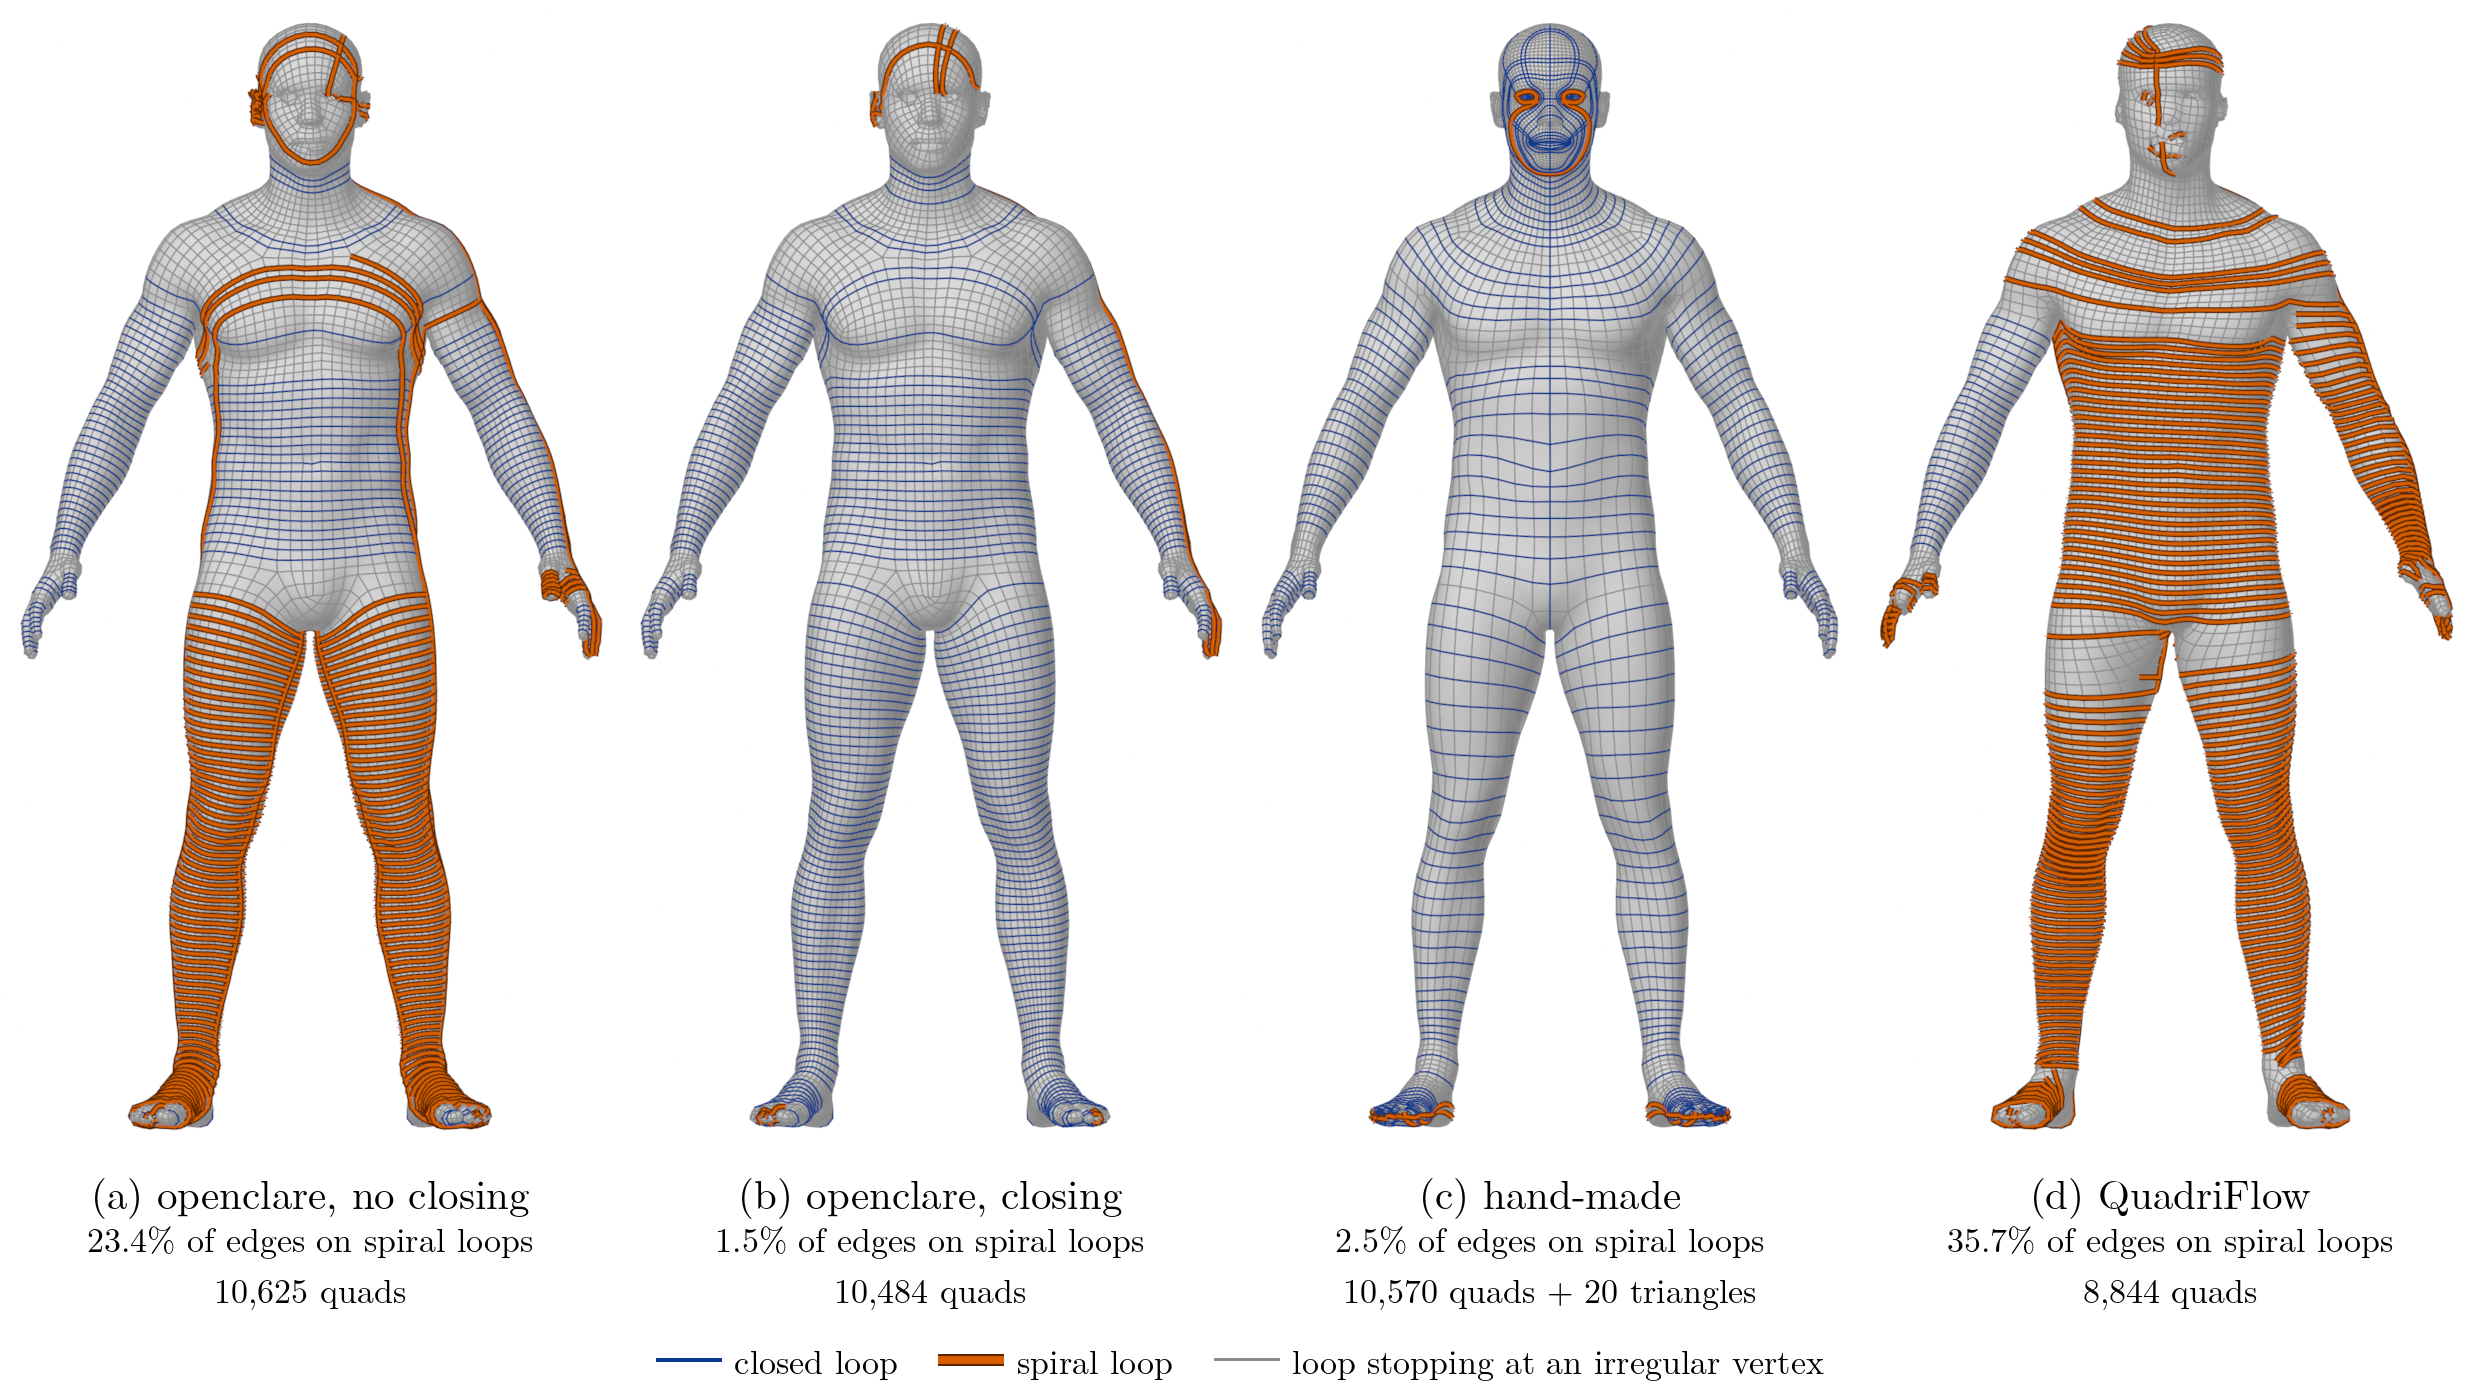
\includegraphics[width=\textwidth]{figures/male-overview.png}
\caption{The male body of the Essentials library, $10{,}590$ quads asked
for: (a)~openclare without closing, (b)~openclare with the closing of
Section~\ref{sec:closing}, (c)~the base mesh modelled by hand,
(d)~QuadriFlow run through Blender, on the source scaled by $100$ and scaled
back: Blender refuses the sculpt as it is, some of its edges being shorter
than its threshold of $10^{-4}$, and QuadriFlow does not depend on the scale.
Edge loops are coloured by their kind in
the measure of Section~\ref{sec:measure}: closed loops dark blue, spiral
loops vermillion (wider, with a dark rim), loops that stop at an irregular
vertex grey. Meshes (a) and (b) come from the engine of version 0.7.0, one
deterministic run each, the runs quoted in the text. Measured on the whole
meshes, they have $10{,}625$, $10{,}484$, $10{,}570$ (plus $20$ triangles)
and $8{,}844$ quads, $23.4\%$ ($21$ loops), $1.46\%$ ($11$), $2.55\%$ ($3$)
and $35.7\%$ ($43$) of their edges on spiral loops, which the panels round to
one decimal, and $17.2\%$, $36.5\%$, $31.6\%$ and $2.7\%$ on closed loops.
QuadriFlow's mesh has $3$ inverted faces and a Hausdorff distance of
$31$\textperthousand\ of the diagonal.}
\label{fig:overview}
\end{figure*}

\begin{figure*}[t]
\centering
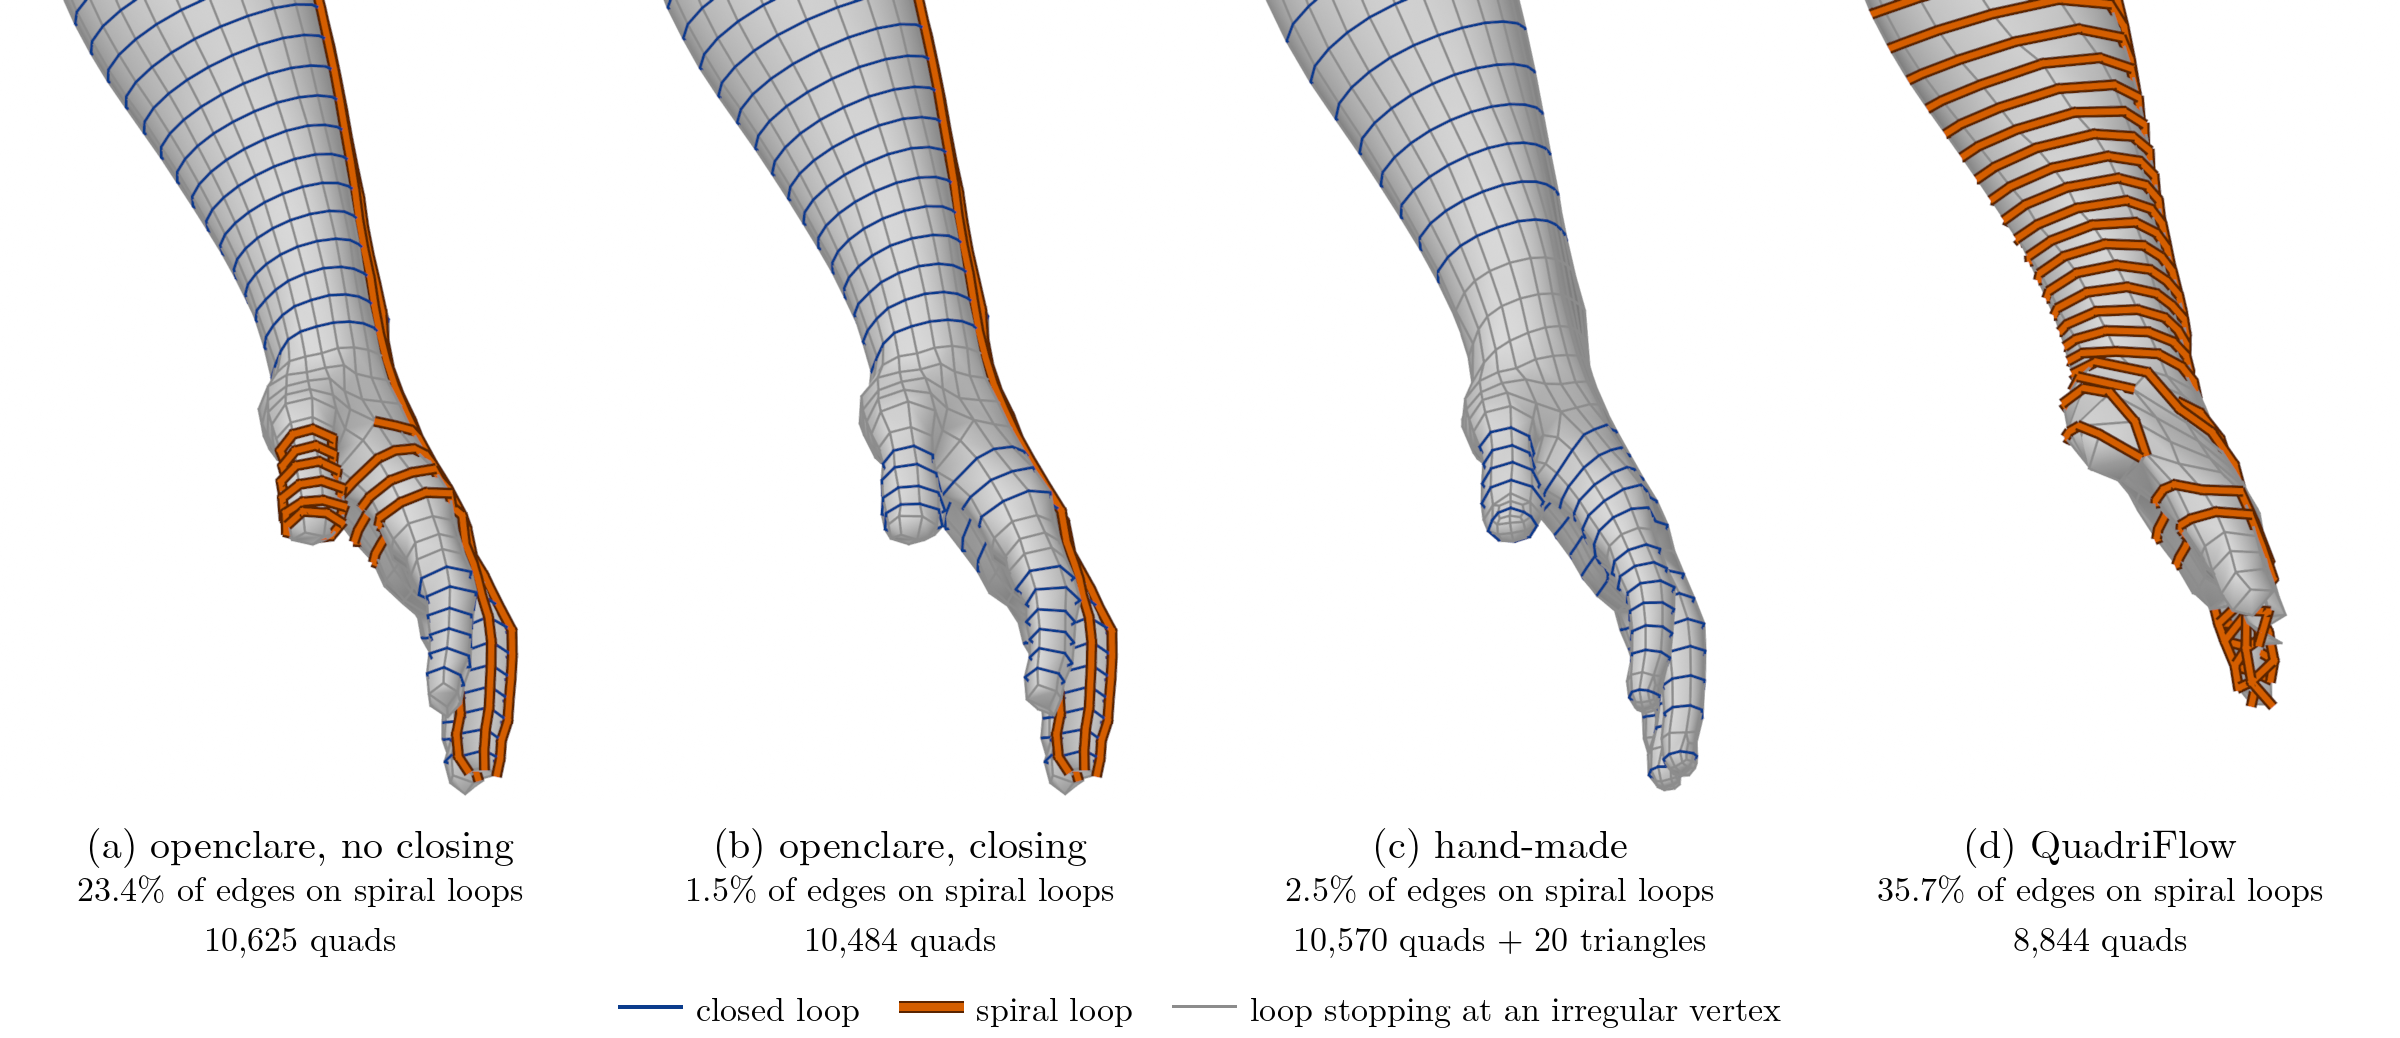
\includegraphics[width=\textwidth]{figures/male-wrist.png}\\[0.6em]
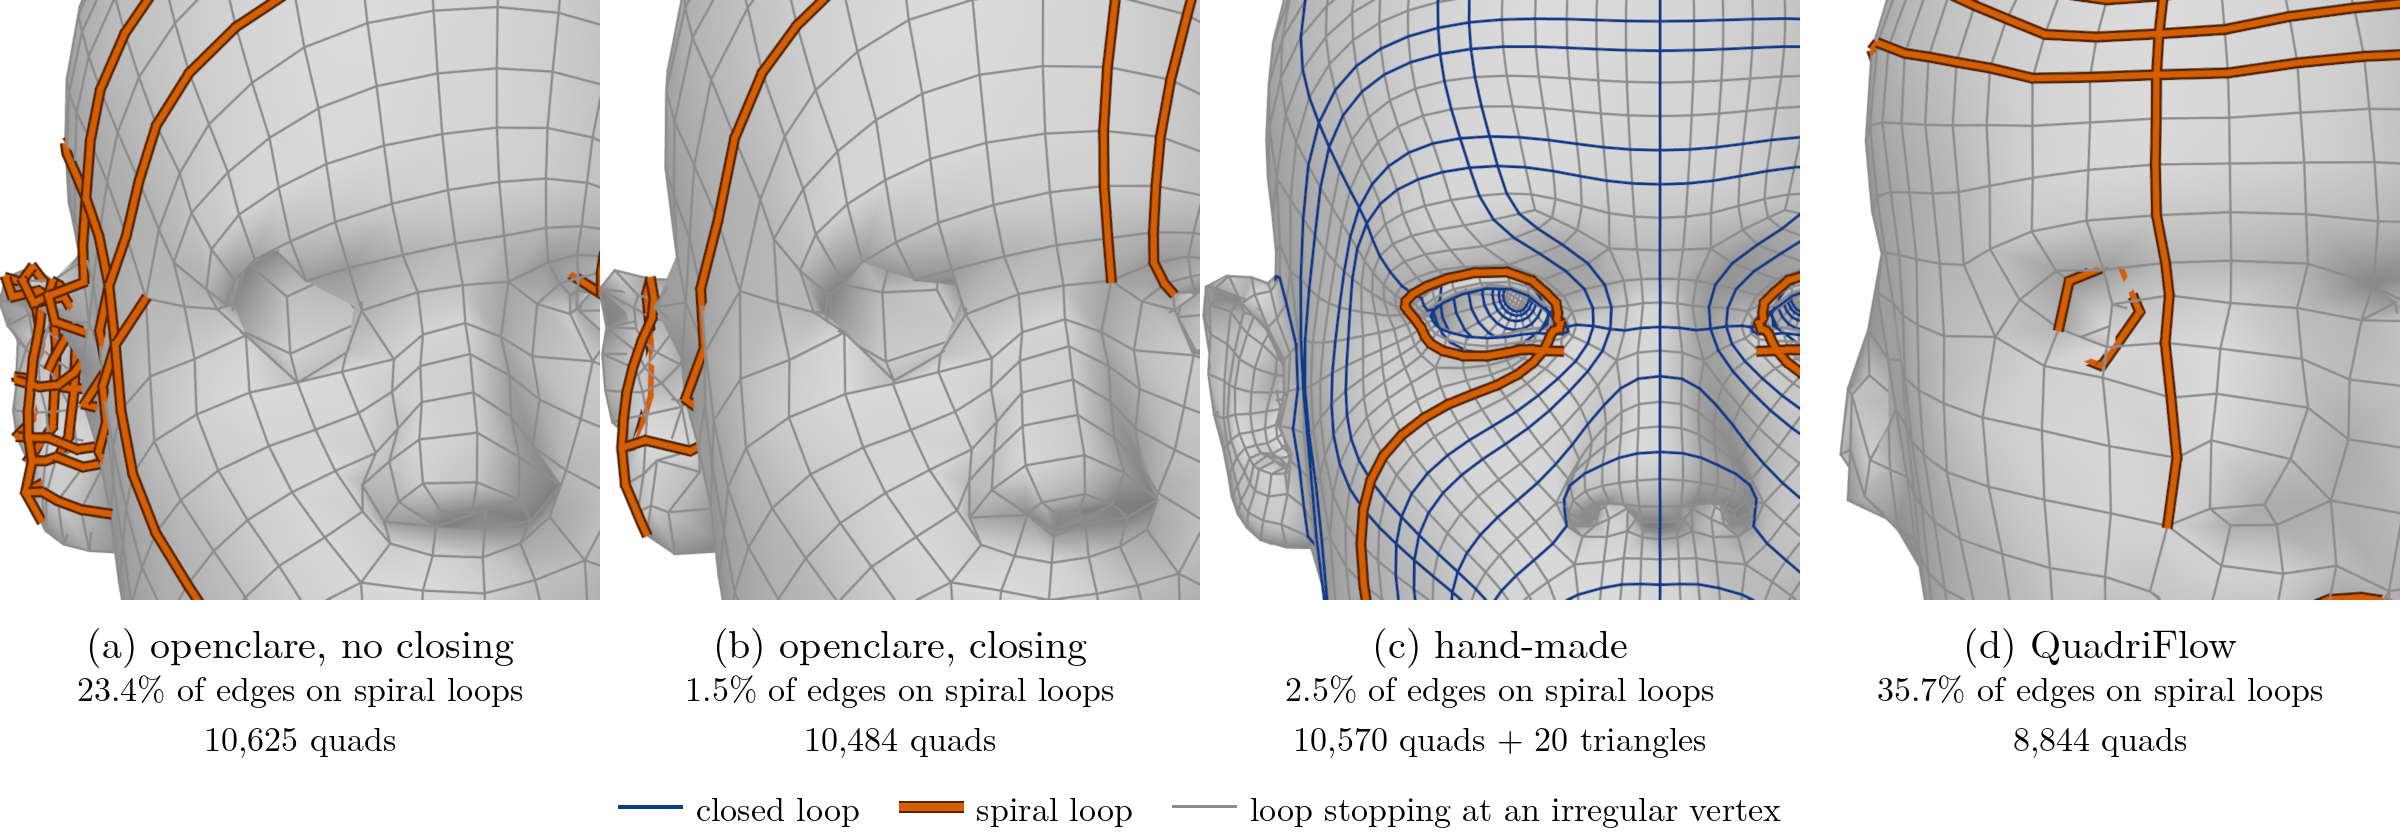
\includegraphics[width=\textwidth]{figures/male-eye.png}
\caption{Close-ups of the four meshes of Figure~\ref{fig:overview}, in the
same order and colours: the left wrist and hand (top; the body's left, on
the viewer's right in Figure~\ref{fig:overview}) and the right eye
(bottom). At the wrist, mesh~(b) has closed loops on the thumb and the back
of the hand where mesh~(a) has spiral ones, and a spiral loop along the outer
side of the forearm remains on both. At the eye, neither openclare mesh has
a spiral loop near the eye, both keep spiral loops on the forehead and at the
ear, and the loop round the eye of the hand-made mesh is itself counted as
spiral.}
\label{fig:closeups}
\end{figure*}

\section{An exact look at the closing system}\label{sec:exact}

How far is the heuristic of Section~\ref{sec:closing} from what the
constraints allow? An experiment option of the engine exports, for each way
of finding turns, the system it works on; we export it for the male body at
$10{,}590$ quads, from the engine as it runs. Its T-mesh has $1{,}342$ nodes
($1{,}068$ T-junctions, $254$ singular vertices, $131$ of valence three and
$123$ of valence five, and $20$ corners of folds), $2{,}146$ arcs and $806$
patches, hence $1{,}612$ balance equations, one per patch and direction. The
export gives the real lengths, every turn found with its shift (on all
$1{,}708$ turns, composing the crossing maps along the walk gives the
exported shift), and the lower bounds the integer search placed on arcs to
keep singularities apart ($36$ to $197$ arcs held at length one, depending on
the way). These bounds are the engine's choice of
\emph{which} arc of a chain between two singular vertices carries their
separation: validity asks a chain to keep a positive total length, not a
given arc. Every statement below is relative to them. We call
$P_{\mathrm{eng}}$ the balanced lengths that meet them; it is neither a
subset nor a superset of the valid quantizations, since it excludes valid
lengths that put the separation on another arc of the chain and allows
lengths that bring other arcs to zero. The ways are numbered as exported:
way $m + 2j + 4i$ starts from the shares $\{0.5\}$ ($m = 0$) or $\{0.2, 0.5,
0.8\}$ ($m = 1$), with the lean bound $0.05$ ($j = 0$) or $0.12$ ($j = 1$)
and the length bound $2$ ($i = 0$) or $6$ ($i = 1$) sides. Without the
other draws the engine keeps way~2 for this body ($1.65\%$ of spiral edges);
with them it keeps the lengths of another draw ($1.46\%$).

\paragraph{The conflict is real but local.}
All held turns can be closed together if the lengths are only asked to be
non-negative; with the bounds of separation, they cannot. By Farkas' lemma a
set of turns cannot be closed within the bounds exactly when some
combination of their shifts equals, modulo the balances, a non-negative
combination of arc lengths that charges an arc held open, and the companion
paper~\cite{gardent2026turns} reads these certificates on the singularities.
In seven ways (all but way~4) some held turn cannot even be closed on its
own. In five of them (0, 1, 2, 5 and 7) it is the same turn, of length
$6.76$, whose shift equals, modulo the balances, $-(\ell_{1892} +
\ell_{1908})$, where arc $1908$, less than $0.09$ quad edges long in the
parametrization, is held at length at least one; in ways 2, 3, 6 and 7 a
second turn, of length $4.72$, is held up in the same way by arc~$1006$ (both
certificates checked in exact rational arithmetic).
Whether $\ell_{1908} = 0$ would merge two singular vertices, that is whether
every valid quantization meets this bound, we did not check. Giving up the
least total amount of the bounds needed to close all held turns, a linear
program, shows that in way~0 the bound of arc $1908$ alone stands in the
way, in way~2 three bounds, that one among them, and in the other ways $6$
to $154$.

\paragraph{How many held turns can close.}
With every bound kept, the largest set of held turns that can be closed
together is found by a mixed-integer program with one binary per turn
(Table~\ref{tab:exact}). The projection of the engine keeps every held turn
closed: its active set asks the lengths to be non-negative only, which, as
above, lets all held turns close; the bounds of separation return in the
integer search. In whole numbers, the same mixed-integer program, with a
limit of fifteen minutes a way, proves its optimum in way~3 only ($90$
turns, as in real numbers); in the other ways it stops with $1$ to $88$
turns fewer than in real numbers.

\begin{table}[t]
\centering
\begin{tabular}{lrr}
\toprule
way & held & closable together \\
\midrule
0 & 58 & 57 \\
1 & 92 & 87 \\
2 & 64 & 61 \\
3 & 102 & 90 \\
4 & 125 & 120 \\
5 & 219 & 189 \\
6 & 131 & 123 \\
7 & 229 & 192 \\
\bottomrule
\end{tabular}
\caption{Male body at $10{,}590$ quads, real numbers, engine of version
0.7.0. ``Closable together'': the largest set of held turns closable with
every bound of separation kept; in way~7 the program stopped at its limit
of $300$ seconds, with a bound of $195$.}
\label{tab:exact}
\end{table}

\paragraph{The rounding ignores the shifts.}
Feeding the integer search of the engine better targets shows what survives
it (Table~\ref{tab:rounding}). The active-set projection, the engine's,
keeps every held turn closed in real numbers, yet after the integer search
$33\%$ to $74\%$ of them are shifted again ($170$ of $229$ in way~7); with a
least-squares projection whose negative lengths are clamped to zero, too,
about $40\%$ of the turns it closes are shifted after the integer search.
The integer search follows the targets but not the shifts. Aiming at the
lengths of the linear program, whose weighted $L^1$ objective puts the
changes on few arcs, the engine ranks first a candidate with $2.63\%$ of
spiral edges, yet outputs the mesh of the plain lengths: after meshing, the
candidates ranked before them were set aside.

\begin{table}[t]
\centering
\small
\begin{tabular}{lrrr}
\toprule
targets of the integer search & turns closed in reals & still shifted after & spiral edges (mesh) \\
\midrule
projection, clamped & 41--52 & 15--25 of them & 2.11\% \\
linear program, $L^1$ & 57--192 & 14--133 of them & 23.39\% \\
active set, floor 0 (the engine) & all held (58--229) & 19--170 of them & 1.46\% \\
active set, floor half the real length & 51--132 & 19--93 of them & 2.80\% \\
\bottomrule
\end{tabular}
\caption{Male body at $10{,}590$ quads, engine of version 0.7.0 with its
experiment options, one run each; ranges over the eight ways. The mesh keeps
the candidate with the fewest spirals, so its share is that of a single way
or draw; with the linear program it is the mesh of the plain lengths.}
\label{tab:rounding}
\end{table}

\paragraph{Whole lengths are not what is missing.}
The balances are the incidence matrix of a bidirected graph whose nodes are
the balance equations and whose edges are the arcs (each arc lies on a side
of each of the two patches it borders). When this graph is connected and has
a cycle that $\pm1$ values cannot balance, as on the body, the companion
paper shows that a set of free arcs parametrizes the lattice of whole
balanced lengths: here $2{,}146 - 1{,}612 = 534$ arcs can be given any whole
lengths and the others follow, so balances alone never obstruct whole
lengths. Closing exactly, in whole numbers, the turns found closable
together, HiGHS finds such lengths in $83$ to $228$ seconds in ways 0 to 3,
and none within ten minutes in ways 4 to 7. The solutions leave $1$, $5$,
$3$ and $12$ held turns shifted where the engine leaves $19$, $40$, $23$ and
$52$, and fewer of the turns not held as well ($3$ against $15$, $9$ against
$25$, $5$ against $18$, $11$ against $34$), at a weighted deviation from the
real lengths $2\%$ to $64\%$ higher. Yet three of the four spiral
\emph{more}, by the engine's count on the connectivity of their lengths:
$5.9\%$, $2.8\%$ and $7.8\%$ of their edges against $4.1\%$, $1.7\%$ and
$3.5\%$ for the engine's lengths in ways 0, 2 and 3; in way~1, $4.9\%$
against $9.1\%$. Only those of way~2 stay within the engine's window of
sizes; the others have $10{,}857$, $12{,}420$ and $11{,}011$ quads. Most of
the loops that spiral are not turns the sampled walks find.

Walking every strip of the mesh of way~2 instead
(Proposition~\ref{prop:complete}) finds $306$ ways round, each strip twice,
once in each direction; $236$ come back shifted. Selecting them by lean, as
the constraint rounds do, keeps $298$, of which $270$ ($135$ strips) can be
closed together in real numbers with every bound kept. Posed directly to
HiGHS, they gave no whole solution in $12{,}651$ seconds; given the $341$
arcs that every real solution sets to zero (each certified by a non-negative
combination of shifts, $216$ certificates over $36$ distinct sets of rings),
none was found in $2{,}596$ seconds either. No real lengths closing the
$270$ rings have a mean deviation from the targets below $1.304$, where the
engine allows $0.522$ ($0.2$ above the $0.322$ of its plain search). The
largest subset closable within a mean deviation of $0.4$, the number of
quads held to first order, found by a program stopped after $600$ seconds,
has $228$ rings (at most $267$) and closes at $0.395$ in real numbers. In
whole numbers, with the reformulation of Aardal, Hurkens and
Lenstra~\cite{aardal2000diophantine} on an LLL-reduced
basis~\cite{lenstra1982lll} of the lattice of closed quantizations, HiGHS,
stopped after $1{,}200$ seconds, finds whole lengths closing all $228$
within every bound at a mean deviation of $0.535$ and $10{,}653$ quads, and
proves that none does better than $0.518$. These lengths lie above the
engine's cap ($0.535$ against $0.522$), so the engine does not take them as
a candidate. Rounding costs between $0.123$ (proven) and $0.140$ (found) of
mean deviation above the real optimum.

\paragraph{The heuristic leaves most of the gap.}
The companion paper~\cite{gardent2026turns} computes the least number of
held turns that any lengths in $P_{\mathrm{eng}}$ leave shifted, a minimum
cover of the irreducible infeasible subsystems~\cite{parker1996iis}: exactly
$1$, $5$, $3$, $12$, $5$, $30$, $8$ and $37$ in ways 0 to 7, against $19$,
$40$, $23$, $52$, $61$, $154$, $72$ and $170$ left shifted by the engine.
With the engine's cap on the deviation and its window of sizes ($10{,}379$
to $10{,}801$ quads) added, at whole lengths, the least number is still
exactly one in way~0 and three in way~2: whole lengths closing every other
held turn exist at $10{,}730$ and $10{,}435$ quads, at mean deviations
$0.387$ and $0.506$. Of the $23$ turns of way~2 the engine leaves shifted,
the bounds of separation force three and the cap, the size and integrality
none; the heuristic accounts for $20$. Closing more turns, however, is not
what the measure of spirals sees: a local search over whole lengths within
the same cap and size closes $45$ more strips of the mesh of way~2 than the
engine does, but at its lengths, where the strips are other walks, $4.7\%$
of the edges spiral, against $1.7\%$ at the engine's lengths of way~2; it is
the choice of the turns to close, at the lengths where they are the strips
of the mesh, that decides how much the mesh spirals. Choosing the most turns to close
is NP-hard for bidirected balances with $0$--$1$ bounds, the algebraic form
of quantization~\cite{gardent2026turns}; whether the balances and turns of an
actual T-mesh stay hard is open.

\paragraph{Closing the most rings, end to end.}
We measured what an exact selection buys on the bench with the slow quality
mode of the engine (\texttt{--quality slow}), against the engine without its
other draws ($5.85\%$ of spiral edges over the $36$ runs), with three
($5.43\%$) and with its twelve ($4.92\%$). For the lengths the engine keeps,
a mixed-integer program closes as many of its strips leaning less than
$0.12$ as it can, weighted by their length round, within the balances, the
bounds of separation, the cap and the quad budget. A strip counts as closed
only where the corridor inequalities~\eqref{eq:corridor} hold for it, so
that it keeps its walk at the new lengths. The engine meshes the result, the
strips are walked again at the new lengths, and the program solved again,
three rounds; each round's lengths join the engine's candidates on the same
terms. The program is solved by HiGHS linked into the engine, each solve
stopped at a work limit (simplex iterations times arcs) that does not depend
on the load. Without the other draws, the slow mode lowers the mean to
$4.41\%$: lower on $9$ of the $36$ runs, never higher. Closed loops ($36.6\%$
against $35.4\%$ of the edges) and mean distance ($0.382$\textperthousand\
in both) barely move, and all $36$ meshes are valid. Against the twelve
other draws it is lower on average ($4.41\%$ against $4.92\%$) but not run
by run: higher on $9$ runs, lower on $5$. On the male body its three rounds
return the lengths they start from: $1.65\%$, as without it, against
$1.46\%$ for the engine with its draws. The gain does not need a solver that
finishes: $90$ of the $120$ solves stop at the work limit, and with a limit
of $5$ seconds per solve instead, $76$ of $100$ stop at it, $18$ of the $66$
rounds (against $12$) return the lengths they start from, and the mean is
$4.56\%$, on four processors where the other runs had eight.

\paragraph{Acting before quantization.}
Moving singular vertices in the parametrization, and rotating the field
cylinder by cylinder, were also tried, with prototypes of the engine that are
not part of it; neither lowered the share of spirals. The Burgers sum of the
companion paper~\cite{gardent2026turns} accounts for it: the shifts of two
parallel turns differ by the across component of the Burgers vector of the
singular vertices between them, which depends only on their developed
positions, so closing one turn by a local change of the map moves its shift
onto the turns beside it. The conflicts are better attacked in quantization.

\section{Limitations and open problems}\label{sec:limits}

The results come from one implementation and are preliminary. The spiral
share of a single model is chaotic, so only the means over three budgets are
robust; the other figures are single runs. The measure sees helices of pitch
up to four only. The exact look covers one body and holds relative to the
engine's bounds of separation, which are its choice of arcs and neither a
subset nor a superset of the valid quantizations. The machine was shared:
its load is recorded, not controlled, and the outcomes that depend on a
time limit depend on it.

Three problems remain open. \emph{An exact formulation}: minimizing the
deviation subject to the balances, the bounds and $\shift_\gamma(\ell) = 0$
for a set of turns is a minimum-deviation flow with linear side constraints;
how much of the exact machinery of~\cite{heistermann2023bimdf} carries over is
open, and the linear relaxation already closes $84\%$ to $98\%$ of the held
turns.
\emph{Closing in whole numbers}: whole lengths closing every ring asked for
are found through a reduced lattice basis, but in minutes, with the number
of quads held only to first order and $0.12$ to $0.14$ above the real optimum
in deviation, here above the engine's cap; can the integer search move within this lattice at the speed of
a flow solver? \emph{Which turns}, the central one on the evidence of
Section~\ref{sec:exact}: closing rings changes the lengths, the lengths
change the strips, and the strips of the new mesh are other walks. Is there a
finite set of turns whose closing implies that every loop of the quad mesh
closes? Can the loops of the quad mesh be read off the T-mesh and its lengths
directly, so that every one is accounted for? Which objective, short of all
loops, predicts the spirals the measure sees?

\section*{AI assistance}
This note and the software it describes were made by a human author working
with an AI system, which is not an author. The author chose the problem and
its aims (edge loops that close into rings and, as an artist, few singular
vertices and few spirals rather than perfectly square quads, quads only), set
the direction and the order of the work, decided which results to pursue and
which changes to merge, and judged the results through the measurements,
pictures and drafts presented to him. Claude Opus 5.5 (Anthropic), used
through Claude Code in October 2026 with several sub-agents in parallel,
wrote the changes to the engine and the experiment scripts, ran all the
experiments and exact computations, searched the literature, stated and
proved the propositions, and drafted the text. References were checked for
existence, and the note of each bibliography entry says how much of the work
was read. A work of which only the abstract, or a review, was read is cited only for what that abstract or review states. Weaker forms of Propositions~\ref{prop:linear}
and~\ref{prop:complete} are checked in Lean~4~\cite{demoura2021lean4} in the
companion paper, as the tag above each says; everything else here not checked by machine was written
with AI help and checked by AI agents rereading it and testing it on the
data, not by a human expert. The note has not been peer reviewed; the author,
who publishes it, is responsible for its content.

\bibliographystyle{plainnat}
\bibliography{refs}

\appendix

\section{Provenance of the figures}\label{app:provenance}

Every figure comes from the engine of version 0.7.0 (commit
\texttt{e13fadb}), built in release mode, and from the scripts of
\nolinkurl{docs/research/closing-loops/experiments/} (those of
Section~\ref{sec:exact} in its folder \nolinkurl{exact/}) and, for the
census, the conflicts and the least number of turns left shifted, which the
companion paper shares, of \nolinkurl{docs/research/turns-of-a-t-mesh/experiments/}.
Each script writes a summary, \texttt{results/}\textit{name}\texttt{.json}
beside it, with the engine's commit and build, the machine, its load and the
solver's version; its README gives the command of every table. The raw
output (meshes, exports, logs) is not in the repository.

\begin{center}
\small
\setlength{\tabcolsep}{4pt}
\begin{tabular}{@{}>{\raggedright\arraybackslash}p{5.6cm}>{\raggedright\arraybackslash}p{4.6cm}>{\raggedright\arraybackslash}p{4.4cm}@{}}
\toprule
figures & script & summary \\
\midrule
twelve models, three budgets (Section~\ref{sec:experiments})
  & \texttt{twelve\_models.py}, the protocol below
  & \texttt{twelve\_models.json} \\
Table~\ref{tab:dev}
  & \texttt{ablation.py}; its last line gave the $36$ meshes above byte for
  byte
  & \texttt{ablation.json} \\
against other remeshers
  & \texttt{against\_remeshers.py}, from \nolinkurl{bench/results/results.json}
  at \texttt{e13fadb}
  & \texttt{against\_remeshers.json} \\
male body, openclare and hand-made
  & \texttt{male\_body.py}
  & \texttt{male\_body.json} \\
Figures~\ref{fig:overview} and~\ref{fig:closeups}, their numbers
  & \texttt{figures/make\_figures.sh}, \texttt{figure\_numbers.py};
  QuadriFlow through Blender, on the source scaled by $100$ and scaled back
  & \texttt{figures.json} \\
Section~\ref{sec:exact}: the T-mesh, the conflicts, the least numbers left
shifted
  & \texttt{census.py}, \texttt{holonomy.py}, \texttt{conflicts.py},
  \texttt{forced.py} of the companion paper
  & their summaries of the same names \\
Section~\ref{sec:exact}: the other figures and Tables~\ref{tab:exact}
and~\ref{tab:rounding}
  & \texttt{exact/}: \texttt{relaxation.py}, \texttt{most\_closable.py},
  \texttt{rings.py}, \texttt{lattice\_rounding.py}, \texttt{local\_search.py},
  \texttt{remesh.py}
  & their summaries of the same names \\
closing the most rings, end to end
  & \texttt{exact/end\_to\_end.py}
  & \texttt{end\_to\_end.json}; the limit of $5$ seconds:
  \texttt{end\_to\_end-time-5.json} \\
\bottomrule
\end{tabular}
\end{center}

\paragraph{The protocol of the twelve models.} For each model $m$ (creature,
blob, suzanne, spot, pig, ogre, bob, jerry, blub, rock with the preset
\texttt{organic}; cage and part with \texttt{hard-surface}) and each budget
$Q \in \{2{,}970, 3{,}000, 3{,}030\}$: \texttt{openclare remesh}
\texttt{bench/out/}$m$\texttt{/source.obj} \textit{out.obj}
\texttt{--preset} $P$ \texttt{--quads} $Q$, then \texttt{openclare measure}
on the source and the output with \texttt{--target} $Q$ \texttt{--json}; the
figures are the means of \texttt{loop\_edges\_spiral},
\texttt{loop\_edges\_closed}, \texttt{loops\_spiral},
\texttt{mean\_distance} and \texttt{angle\_deviation\_mean} over the $36$
runs.

\paragraph{Reproducibility.} The method is implemented in openclare (Rust),
in the main branch of the repository; the bench is driven by
\texttt{bench/run.py}. The export of the T-mesh and the switches of
Table~\ref{tab:dev} are experiment options of the engine of version 0.7.0
(\texttt{ALGORITHM.md}, ``Experiment options''), and the slow quality mode
is its option \texttt{--quality slow}, so the scripts above make every
figure again on that engine; the figures that
depend on a time limit depend on the machine and its load as well. The
prototypes of ``Acting before quantization'' are not part of the engine and
are not scripted. This version of the note was built from commit
\texttt{\enginecommit}.

\end{document}
 gives the paper
% without them, for a venue that wants it plain.
\newcommand{\lean}[1]{\texttt{\detokenize{#1}}}
\ifdefined\plain
\newenvironment{evidence}[3][]{}{}
\else
\usepackage[most]{tcolorbox}
\newcommand{\evlevel}[2]{\expandafter\newcommand\csname ev-name-#1\endcsname{#2}}
\evlevel{lean}{Lean, complete}
\evlevel{core}{Lean, algebraic core}
\evlevel{data}{Checked on the engine's data}
\evlevel{measured}{Measured}
\evlevel{prose}{Proof on paper only}
\evlevel{tested}{Conjecture, checked by computer}
\evlevel{cited}{Standard, cited}
\evlevel{open}{Open, no claim}
\newcommand{\evname}[1]{\csname ev-name-#1\endcsname}
\tcbset{evstyle-lean/.style={}, evstyle-core/.style={}, evstyle-data/.style={},
  evstyle-measured/.style={}, evstyle-tested/.style={}, evstyle-prose/.style={},
  evstyle-cited/.style={},
  evstyle-open/.style={frame hidden, borderline={0.4pt}{0pt}{black!45, dashed}}}
\newtcolorbox{evidence}[3][]{breakable, enhanced, colback=white,
  colframe=black!45, boxrule=0.4pt, arc=0pt, left=4pt, right=4pt, top=2pt,
  bottom=2pt, before skip=6pt, after skip=6pt, evstyle-#2,
  title={\footnotesize\textsc{\evname{#2}}\if\relax\detokenize{#3}\relax\else
    \quad #3\fi},
  coltitle=black, colbacktitle=white, titlerule=0.4pt, toptitle=1pt,
  bottomtitle=1pt, #1}
\fi

\title{Closing Edge Loops at Quantization Time:\\
Helix Constraints for T-Mesh Quantization\\[0.5em]
\large Research note --- draft, not peer reviewed}
\author{Marc Gardent%
\thanks{This note is distributed under the Creative Commons Attribution
4.0 International licence (CC BY 4.0). The code of openclare is under the
GPL-3.0-or-later of the repository. The note describes the engine at commit
\texttt{\enginecommit} of \url{https://github.com/marcgardent/openclare}.
A French translation is in \texttt{paper.fr.pdf}, beside this note.}\\
\normalsize Independent researcher\\
\normalsize ORCID: \href{https://orcid.org/0009-0000-6466-3098}{0009-0000-6466-3098}\\
\normalsize Contact: through the repository,
\url{https://github.com/marcgardent/openclare}}
\date{October 2026}

\begin{document}
\maketitle

\begin{abstract}
Automatic quad remeshing often produces edge loops that wind round a part of
the shape as helices instead of closing into rings. Bommes et
al.~\cite{bommes2011structure} remove such \emph{q-helices} from a finished
mesh; we prevent them where the integer structure of the mesh is decided, in
the quantization of a T-mesh. A straight walk across the patches of a T-mesh
that returns to its first side, a \emph{turn}, has a \emph{shift} that is an
integer linear form in the arc lengths; at whole lengths it is how far the
strip of quads following the turn comes back beside itself, and every strip
of the mesh is such a walk. We add the constraints that close turns to a
minimum-deviation quantizer~\cite{heistermann2023bimdf}, through a
least-change projection, repair walks and rounds of constraint generation on
the strips of the mesh, and keep the candidate with the fewest spiral edges,
counted by a test that tells helices from closed, open and border loops. Over
twelve models at three budgets near 3{,}000 quads, the engine leaves 4.92\%
of the edges on spiral loops (19.8\% without closing); on the seven models
that two other open-source remeshers also mesh validly, 2.2\% against 38.8\% % NIGHT4
and 21.7\%; on a human body, 1.5\%, against 2.5\% for the hand-made mesh.
An exact analysis of the closing system of that body shows that the conflict between closing
turns and keeping singularities apart is real but local, that the heuristic
rather than the constraints leaves most turns shifted, and that closing more
turns does not by itself make fewer spirals: the strips move with the
lengths, and the choice of the turns to close decides.
\end{abstract}

\section{Introduction}

In our experience, element shape and alignment are rarely what limits
field-aligned quad remeshing today (see the
surveys~\cite{bommes2013survey,campen2017survey}). What remains is structure:
the way edge loops run across the surface. Artists expect a loop round an
arm, a leg or a neck to be a ring. Automatic methods often produce a helix
instead: the loop goes round, comes back one or a few rows further, and winds
along the whole part (Figure~\ref{fig:overview}). Bommes et al.\ showed that
helical configurations are a main reason why the base complex of an otherwise
good quad mesh stays dense~\cite{bommes2011structure}, and removed them from
the finished mesh.

Whether a loop closes is decided upstream, when a quantizer assigns whole
lengths to the arcs of a T-mesh traced in a seamless
parametrization~\cite{campen2015qgp,lyon2021constrained,heistermann2023bimdf}.
Quantizers choose these lengths for consistency, validity and closeness to
the parametrization; the loops close or spiral as a side effect. This paper
constrains the loops in the quantization itself. Section~\ref{sec:turns}
defines \emph{turns}, straight walks across the patches of a T-mesh that
return to their first side, and shows that the \emph{shift} of a turn is an
integer linear form in the arc lengths that gives, at whole lengths, the
pitch of the strip of quads following it, and that every strip of the mesh
is such a walk. Section~\ref{sec:closing} adds the closing of turns to a
minimum-deviation quantizer through a least-change projection, repair walks
and rounds of constraint generation on the strips, with safeguards on folds,
distortion and budget. Section~\ref{sec:measure} gives a share of spiral
edges that tells helices of pitch up to four from closed, open and border
loops; loop counts and loop simplicity scores
exist~\cite{liu2025quadgpt,kong2026squadgen}, but they do not separate
helices from open loops. Section~\ref{sec:experiments} measures the method in
the open-source remesher openclare against two open-source remeshers and a
mesh modelled by hand, and Section~\ref{sec:exact} solves the closing system
of a human body exactly to see where the heuristic stands: the conflict
between closing turns and keeping singularities apart is local, the
heuristic leaves most of the shifted turns that no constraint forces, and
yet closing more turns does not by itself reduce the spirals, because the
strips of the mesh move with the lengths; adding the inequalities of the
corridor makes the count of closed strips exact, a coupling of shift and
corridor we found in no earlier quantizer. Section~\ref{sec:limits} states
the limitations and the open problems.

This work began as a programming project, openclare, an open-source quad
remesher, and became research when engineering alone could no longer tell
which results could be guaranteed and which computations could be saved.
Each result used here answers such a question. The shift of a turn is linear
in the arc lengths, so closing a loop becomes a linear constraint of the
quantizer rather than a test after the fact; its parity follows the length
of the turn, so some repairs are known to be impossible before they are
tried; and choosing the largest set of turns to close is NP-hard in the
algebraic form quantization takes, which is why the engine keeps to a heuristic, with an exact solver only on demand.

The theory behind the conflicts, which reads the shift as translational
holonomy of the flat metric and derives obstructions to closing from the
singularities, a lower bound on the turns every quantization leaves shifted,
and the NP-hardness of choosing the turns to close, is the subject of a
companion paper~\cite{gardent2026turns}; we state its results in one
sentence where we need them, without proof. Statements here are
\emph{proved} when they come with a proof, \emph{measured} when they come
from exact arithmetic or solver output on the systems openclare exports, and
\emph{conjectured} otherwise.

\section{Background and related work}\label{sec:related}

\paragraph{T-mesh quantization.}
Mixed-integer quadrangulation~\cite{bommes2009miq} and integer-grid
maps~\cite{bommes2013igm} decide the integer structure of a quad mesh in
their quantization. Campen et al.\ show that even a valid quantization of a seamless
parametrization is a hard combinatorial problem, and solve it through
systems of linear Diophantine equations~\cite{campen2015qgp}.
Lyon et al.\ solve a constrained version as an integer linear program,
bounding the directional deviation of the separatrices of the resulting
layout, and require, as openclare does, that the quantization keep
singularities apart~\cite{lyon2021constrained}. Heistermann et al.\ cast
quantization as a minimum-deviation flow on a bidirected graph and give a
fast approximate solver and an exact refinement~\cite{heistermann2023bimdf};
openclare follows their formulation. To our knowledge none of these
constrains the helices.

\paragraph{Helices after meshing.}
Bommes et al.~\cite{bommes2011structure} define a \emph{q-helix} as a dual
parametric line with an integer \emph{pitch} $h$ and \emph{turn length}
$\tau$: walking $\tau$ steps along it is equivalent to $h$ side-steps. They
detect minimal q-helices by the self-intersections of orthogonal dual lines
and remove them greedily with grid-preserving operators, closed dual paths of
shift and collapse steps that keep the mesh all-quad and its singularities in
place, followed by tangential smoothing; their experiments remove most
helices (from 17--52 down to 1--23 per model). They note that choosing the
pairs of singularities to align directly in the parametrization is often
complicated or even ambiguous to automate, giving the feature-aligned
T-meshes of Myles et al.~\cite{myles2010feature} as an example. Razafindrazaka and
Polthier~\cite{razafindrazaka2017optimal} replace the base complex of a
finished mesh by an optimal one, found as a perfect matching on a graph over
its singular vertices, and note that the operators
of~\cite{bommes2011structure} leave some spirals. Both work after meshing,
not in the quantization.

\paragraph{Periods round a tube.}
QuadCover~\cite{kalberer2007quadcover} lifts the cross field to a branched
covering where it becomes a vector field. The stripe parameterization of
tubular surfaces~\cite{kalberer2011stripe}, built on it, measures the jump
(``gap'') of the parameter across each cut path and rounds it to the nearest
whole number; the gap across a loop round a tube is what we call the shift of
a turn, and rounded to a non-zero whole number it gives a helix of that
pitch. That paper treats spiralling stripes as a legitimate outcome, and
notes that rounding the gaps for least distortion is a hard combinatorial
problem that it does not solve exactly.

\paragraph{Flat metrics and finite trajectories.}
Declaring every quad a unit square turns a quad mesh into a flat metric with
cone points at its irregular vertices. Chen et al.~\cite{chen2019metric}
characterize the metrics that arise this way; one of their conditions is a
\emph{finite geodesic lamination}, the straight lines of the field being
finite loops, which they assume rather than construct. Lei et
al.~\cite{lei2020quartic} show that a closed quad mesh induces a meromorphic
quartic differential and list as an open problem the guarantee that all its
trajectories are finite. A trajectory that is not finite is precisely an edge
loop that does not close. A quadratic differential all of whose non-critical
trajectories close is a Jenkins--Strebel
differential~\cite{strebel1984quadratic}; the complement of its critical
graph is a union of flat cylinders, and a helix is a cylinder glued back with
a shift of a whole number of rows. On a closed surface the valences $k(v)$ of
a quad mesh satisfy $\sum_v (4 - k(v)) = 4\chi$: with valences three and five only, a
closed human body needs at least eight vertices of valence three, but a hand-made base mesh has
hundreds, and their count says nothing of where the loops go.

\paragraph{Loops by construction.}
Dual loops meshing~\cite{campen2012dual} builds a layout from loops traced on
the surface, which close by construction; Lei et
al.~\cite{lei2017foliation} build quad meshes from a Strebel differential
with prescribed cylinders, and skeleton-guided
layouts~\cite{usai2015skeleton} follow the curve skeleton of an articulated
shape. Myles
et al.~\cite{myles2014robust} trace the field into a partition into patches,
Pietroni et al.~\cite{pietroni2016tracing} extract a layout from traced
field-coherent paths with a binary linear program, and Razafindrazaka et
al.~\cite{razafindrazaka2015perfect} obtain a layout as a minimum-weight
perfect matching. These methods build coarse layouts, or, for Myles et al.,
a parametrization from one; none asks the loops of a dense mesh to close.

\paragraph{Measuring loops.}
QuadGPT~\cite{liu2025quadgpt} counts \emph{quad rings} (closed loops of
faces) and \emph{quad lines} (open strips) and uses them as reward signals
for preference optimization, without telling spirals from open lines.
SQuadGen~\cite{kong2026squadgen} scores the loops of a layout by their
self-intersections and their rotation index, and reports the area share of
simple loops; it does not tell helices from open loops either.

\section{Turns of a T-mesh}\label{sec:turns}

A T-mesh is a partition of the surface into rectangles, the \emph{patches},
whose sides are made of \emph{arcs}; nodes where a trace stops on another are
T-junctions, and the singular vertices of the field are nodes. Each patch
$P$ has local coordinates with its first corner at the origin and its sides
along the axes. A quantization assigns every arc $a$ a length $\ell_a \in
\Z_{\ge 0}$ such that opposite sides of every patch have equal length, the
\emph{balances} $B\ell = 0$; the quad mesh is then read off as the integer
grid of each patch.

\begin{definition}[Turn]
A \emph{turn} $\gamma$ is a straight walk across patches, from an offset of
its first side that meets no node: it enters a patch through a side, leaves
through the opposite side at the same distance from the corresponding
corner, enters the neighbouring patch across the arc it reaches, and so on,
until it comes back into its first patch through its first side.
\end{definition}

\begin{figure}[t]
\centering
% A turn of a T-mesh, its corridor, its shift and the helix it makes.
% \input inside a figure; needs \usepackage{tikz} and
% \usetikzlibrary{arrows.meta,decorations.pathreplacing}.
%
% (a) A band of a T-mesh on a cylinder, cut open along the left side of P_1:
% the right side of P_4 is glued to the left side of P_1, drawn again, dashed,
% where the walk comes back into it. The band continues above and below. Every
% node is at a whole position; the faint grid is the quad mesh at these
% lengths. The turn gamma starts on the left side of P_1 at offset o = 2.5 and
% crosses P_1, P_2, P_3, P_4. Measured from the first (lower) corner of each
% patch, its offset grows by l_b crossing into P_2, drops by l_c into P_3 and
% grows by l_d into P_4; the bottoms of P_4 and P_1 meet at the cut. So it comes
% back into P_1 at o + s with s = l_b - l_c + l_d = 1 - 2 + 2 = 1. The corridor
% (the offsets whose walk crosses the same arcs) is 1 < o < 4.
% (b) The strip of quads at o = 2.5 on the cylinder: each round comes back one
% row beside itself, at o = 1.5, 2.5, 3.5 within the corridor, then leaves it:
% a helix of pitch 1. The numbers are the offsets where the rounds start.
\begin{tikzpicture}[x=0.56cm, y=0.56cm, font=\small,
    side/.style={draw=black, line width=0.6pt},
    ghost/.style={draw=black!55, line width=0.6pt, dashed},
    quadgrid/.style={draw=black!18, line width=0.3pt},
    node dot/.style={circle, fill=black, inner sep=0pt, minimum size=3.2pt},
    arc mark/.style={line width=2.2pt, draw=black},
    turn/.style={line width=1.1pt, draw=black, -{Stealth[length=6pt]}},
    brace/.style={decorate, decoration={brace, amplitude=4pt}, line width=0.6pt}]
  \definecolor{corridor}{HTML}{CFE0F3}
  \definecolor{loopspiral}{HTML}{D55E00}

  % ---------------------------------------------------------------- (a)
  \begin{scope}
    \clip (-0.1,-2.4) rectangle (16.1,7.4);
    % The corridor of the turn, 1 < o < 4, from P_1 round to P_1 again.
    \fill[corridor] (0,1) rectangle (13,4);
    \draw[quadgrid, step={(1,1)}] (0,-3) grid (16,8);
    % Sides of the columns of patches, which run through the band.
    \foreach \x in {0,3,7,10,13} \draw[side] (\x,-3) -- (\x,8);
    \draw[ghost] (16,-3) -- (16,8);
    % The bottom and top of P_1, ..., P_4, and of P_1 again.
    \foreach \x/\X/\b/\t in {0/3/0/5, 3/7/-1/4, 7/10/1/6, 10/13/-1/4} {
      \draw[side] (\x,\b) -- (\X,\b) (\x,\t) -- (\X,\t);
      \foreach \px in {\x,\X} \foreach \py in {\b,\t}
        \node[node dot] at (\px,\py) {};
    }
    \draw[ghost] (13,-1) -- (16,-1) (13,4) -- (16,4);
    \foreach \py in {-1,4} \node[node dot, fill=black!55] at (16,\py) {};
  \end{scope}
  % The arcs whose lengths the shift adds up.
  \draw[arc mark] (3,-1) -- (3,0) node[midway, left=1pt] {$b$};
  \draw[arc mark] (7,-1) -- (7,1) node[midway, left=1pt] {$c$};
  \draw[arc mark] (10,-1) -- (10,1) node[midway, right=1pt] {$d$};
  % Patch names.
  \node at (1.5,4.5) {$P_1$};
  \node at (5,0) {$P_2$};
  \node at (8.5,5) {$P_3$};
  \node at (11.5,0) {$P_4$};
  \node[black!60] at (14.5,3.35) {\footnotesize $P_1$ again};
  % The turn, from offset o = 2.5 of the first side of P_1.
  \draw[turn] (0,2.5) -- (13.08,2.5);
  \node[above] at (6.4,2.5) {$\gamma$};
  \draw[black, line width=0.6pt, fill=white] (0,2.5) circle (2.2pt);
  % Where it comes back: in the frame of P_1, at o + s.
  \draw[black!60, dashed, line width=0.8pt] (13,2.5) -- (16,2.5);
  \draw[black!60, dotted, line width=0.9pt] (13,1.5) -- (16,1.5);
  \draw[black, line width=0.6pt, fill=white] (13,1.5) circle (2.2pt);
  \node[right, inner sep=1pt] at (16.15,2.5) {\footnotesize $o + s_\gamma(\ell)$};
  \node[right, inner sep=1pt] at (16.15,1.5) {\footnotesize $o$};
  \draw[brace, decoration={mirror}] (15.7,1.5) -- (15.7,2.5)
    node[midway, left=4pt, inner sep=1pt] {\footnotesize $s_\gamma$};
  % Offset and corridor on the first side.
  \node[left] at (-0.05,2.5) {$o$};
  \draw[brace] (-0.9,1) -- (-0.9,4) node[midway, left=4pt, rotate=90, anchor=south]
    {\footnotesize corridor};
  % The shift as a linear form of the arc lengths.
  \node[anchor=north west] at (0,-2.7)
    {$s_\gamma(\ell) = \ell_b - \ell_c + \ell_d = 1 - 2 + 2 = 1$};
  \node[anchor=north] at (8,-4.2) {(a)};

  % ---------------------------------------------------------------- (b)
  % The strip of quads at o = 2.5 on the cylinder, seen from slightly above:
  % a helix of pitch |s| = 1 row, three rounds in the corridor, 13 quads a
  % round (the length of the turn).
  \begin{scope}[shift={(22.4,-1.6)}]
    \pgfmathsetmacro{\R}{1.9}   % radius
    \pgfmathsetmacro{\k}{0.2}   % flattening of the ellipses
    \pgfmathsetmacro{\w}{1.15}  % one row of quads
    \pgfmathsetmacro{\H}{7.0}   % height
    \pgfmathsetmacro{\zz}{1.4}  % bottom of the first round
    % Back halves: the centre line of the strip, seen through the cylinder.
    \foreach \j in {0,1,2} {
      \draw[loopspiral!80, dashed, line width=0.7pt]
        plot[domain=360*\j+180:360*\j+360, samples=40, variable=\t]
          ({\R*cos(\t)}, {\zz + \w*(\t/360 + 0.5) - \k*\R*sin(\t)});
    }
    % The cylinder, translucent.
    \fill[black!25, fill opacity=0.18] (-\R,0) -- (-\R,\H) arc[start angle=180, end angle=360,
      x radius=\R, y radius=\k*\R] -- (\R,0) arc[start angle=0, end angle=-180,
      x radius=\R, y radius=\k*\R] -- cycle;
    \draw[line width=0.6pt] (-\R,0) -- (-\R,\H) (\R,0) -- (\R,\H);
    \draw[line width=0.6pt] (0,\H) ellipse[x radius=\R, y radius=\k*\R];
    \draw[line width=0.6pt] (\R,0) arc[start angle=0, end angle=-180,
      x radius=\R, y radius=\k*\R];
    \draw[line width=0.4pt, black!40, dashed] (\R,0) arc[start angle=0, end angle=180,
      x radius=\R, y radius=\k*\R];
    % Front halves: the quads of the strip, 13 a round, and its centre line.
    \foreach \j in {0,1,2} {
      \fill[loopspiral!35, fill opacity=0.55]
        plot[domain=360*\j:360*\j+180, samples=40, variable=\t]
          ({\R*cos(\t)}, {\zz + \w*\t/360 - \k*\R*sin(\t)})
        -- plot[domain=360*\j+180:360*\j, samples=40, variable=\t]
          ({\R*cos(\t)}, {\zz + \w*(\t/360 + 1) - \k*\R*sin(\t)}) -- cycle;
      \foreach \e in {0,1} {
        \draw[loopspiral!70, line width=0.5pt]
          plot[domain=360*\j:360*\j+180, samples=40, variable=\t]
            ({\R*cos(\t)}, {\zz + \w*(\t/360 + \e) - \k*\R*sin(\t)});
      }
      \foreach \q in {1,...,6} {
        \pgfmathsetmacro{\t}{360*\j + \q*360/13}
        \draw[loopspiral!70, line width=0.4pt]
          ({\R*cos(\t)}, {\zz + \w*\t/360 - \k*\R*sin(\t)}) --
          ({\R*cos(\t)}, {\zz + \w*(\t/360 + 1) - \k*\R*sin(\t)});
      }
      \draw[loopspiral, line width=1.1pt, -{Stealth[length=5pt]}]
        plot[domain=360*\j:360*\j+176, samples=40, variable=\t]
          ({\R*cos(\t)}, {\zz + \w*(\t/360 + 0.5) - \k*\R*sin(\t)});
      % The offset on the first side where the round starts.
      \pgfmathsetmacro{\n}{\j + 1.5}
      \node[right, font=\scriptsize, inner sep=2pt] at (\R,\zz + \w*\j + 0.5*\w)
        {$\pgfmathprintnumber[fixed, precision=1, fixed zerofill]{\n}$};
    }
    \node[anchor=north, align=center, font=\footnotesize] at (0,-0.5)
      {the strip at $o = 2.5$: one helix\\ through $o = 1.5$, $2.5$, $3.5$,\\ pitch $|s_\gamma(\ell)| = 1$};
  \end{scope}
  \node[anchor=north] at (22.4,-4.2) {(b)};
\end{tikzpicture}

\caption{A turn and the helix it makes. (a)~A band of a T-mesh on a
cylinder, cut open along the first side of $P_1$, which is drawn again,
dashed, past $P_4$, where it is glued; every node is at a whole position and
the faint grid is the quad mesh at these lengths. The turn $\gamma$ leaves
the first side at offset $o$ and crosses $P_1$ to $P_4$; measured from the
first corner of each patch, its offset grows by $\ell_b$, drops by $\ell_c$
and grows by $\ell_d$, so it comes back at $o + \shift_\gamma(\ell)$ with
$\shift_\gamma(\ell) = \ell_b - \ell_c + \ell_d = 1$. The corridor
(shaded), the offsets whose walk crosses the same arcs, is $1 < o < 4$.
(b)~The strip of quads at $o = 2.5$ on the cylinder: each round comes back
one row beside itself, through $o = 1.5$, $2.5$ and $3.5$, then leaves the
corridor: a helix of pitch $1$ (Proposition~\ref{prop:linear}).}
\label{fig:turn}
\end{figure}

Crossing from patch $P$ to patch $Q$ across an arc composes a quarter-turn
rotation of the local frame with a translation whose components are signed
sums of arc lengths along the rims of $P$ and $Q$, the position of a rim
point being the sum of the lengths of the arcs between it and the first
corner.

\begin{evidence}{core}{\lean{TMesh.Turn.shift_linear}, \lean{TMesh.Turn.mem_corridor_iff}, \lean{TMesh.Turn.comes_back}, \lean{TMesh.Turn.winds}; examples: \lean{TMesh.twistedTorus.walk_turn}; assumed: an oriented gluing; the corridor without half-integers is not formalized}
\begin{proposition}[The shift of a turn is linear]\label{prop:linear}
For a turn $\gamma$ there are integer coefficients $c_a$, independent of the
lengths, such that after a full turn a point of the first side has moved
across the walking direction by
\[
  \shift_\gamma(\ell) = \sum_a c_a\, \ell_a .
\]
For whole lengths $\ell$, let $o$ be a half-integer offset of the first side
whose walk at the lengths $\ell$ crosses the same patches as $\gamma$ (the
set of such offsets is the \emph{corridor} of $\gamma$ at $\ell$). Then the
dual line of the quad mesh at $o$ comes back at $o + \shift_\gamma(\ell)$:
it closes after one round if and only if $\shift_\gamma(\ell) = 0$. If
moreover $o + j\,\shift_\gamma(\ell)$ lies in the corridor for $j = 1, \dots,
t - 1$, it winds $t$ times round as a helix of pitch $|\shift_\gamma(\ell)|$
in the sense of~\cite{bommes2011structure}.
\end{proposition}
\end{evidence}

\begin{proof}[Sketch]
Each crossing is a map $x \mapsto R^k x + t$ with $R$ the quarter-turn and
$t$ a vector whose entries are sums of $\pm\ell_a$. The walk re-enters its
first side inward, so the composition along $\gamma$ has trivial rotation and
is a translation $T_\gamma(\ell)$, linear in $\ell$ with integer
coefficients. Its component along the walking direction does not move a
point of the first side off that side; its component across is
$\shift_\gamma(\ell)$. Singularities are nodes, never inside a patch, so the
quad mesh is a regular grid along the walk, and a dual line at distance $o$
from the first corner, as long as it crosses the same patches as $\gamma$,
comes back at distance $o + \shift_\gamma(\ell)$.
\end{proof}

The component of $T_\gamma(\ell)$ along the walking direction is the
\emph{length} $\alpha_\gamma(\ell)$ of the turn, also an integer linear form,
which at whole lengths is the number of quads of the strip in one turn. The
shift is the across component of the translational holonomy of the flat
metric along the turn; for a ring of quads it is the
twist of a cylinder. What is specific here is its expression in the arc
lengths of a T-mesh, as a constraint of the quantization. The companion
paper~\cite{gardent2026turns} shows that it is set by the singularities: for
a turn whose curve is simple, it equals up to sign the across component of
the Burgers vector of the singular vertices on one side, so that two parallel turns bounding an annulus free
of singular vertices have the same shift, and a helix is a property of a
whole cylinder of turns, not of one of them. In openclare
(\texttt{quantization/tubes.rs}) the shift is built once per turn as an
expression in the arc lengths, by composing the rim expressions of the
crossed patches; evaluated at the real lengths of the parametrization it
gives the \emph{real shift}, the twist the field itself gives the cylinder.
Figure~\ref{fig:turn} shows a turn, its corridor and the helix its shift
makes.

The closing constraint $\shift_\gamma(\ell) = 0$ thus speaks of a fixed
sequence of crossed patches, and describes a strip of the mesh only together
with the corridor. Explicitly, let $\gamma$ cross the arcs $a_1, \dots, a_m$
in turn; the walk from offset $o$ crosses the side holding $a_j$ at the
distance $\epsilon_j o + q_j(\ell)$ from its first corner, with $\epsilon_j =
\pm 1$ and $q_j$ an integer linear form, and $a_j$ starts at the distance
$e_j(\ell)$, a sum of arc lengths. At whole lengths and for a half-integer
$o$, the corridor is cut out by the inequalities
\begin{equation}\label{eq:corridor}
  e_j(\ell) + \tfrac12 \;\le\; \epsilon_j\, o + q_j(\ell) \;\le\; e_j(\ell) +
  \ell_{a_j} - \tfrac12, \qquad j = 1, \dots, m,
\end{equation}
two per crossing. The closing steps of Section~\ref{sec:closing} impose the
shifts but not these inequalities; Section~\ref{sec:exact} measures what
this costs. The strips themselves are all walks of this kind.

\begin{definition}[Strip]
For whole lengths $\ell$ balancing every patch, with every patch side
positive and no two singular vertices at the same point, the quad mesh is, in
each patch, the integer grid of its sides. A \emph{strip} is a maximal
sequence of quads, each sharing with the next the edge opposite the one it
shares with the previous.
\end{definition}

\begin{evidence}{core}{\lean{Completeness.completeness_at_given_lengths}, in a model; assumed: integer rectangles glued along their arcs by $t \mapsto \pm t + c$, $c$ whole; a closed surface, crossing an arc taking the unit edges of a side one to one onto unit edges; that the cycles of the model are the strips of the mesh; the strips that reach a border are not formalized}
\begin{proposition}[Completeness at given lengths]\label{prop:complete}
Let $\ell$ be as in the definition. Every strip of the quad mesh that
crosses a side $\sigma$ of a patch $P$ at the quad edge $[k, k+1]$ of
$\sigma$ is the walk taken \emph{with the lengths $\ell$} from $\sigma$ at
offset $k + \tfrac12$. On a closed surface the strips are thus the cycles of
the walk on the half-integer stations of all sides, each oriented strip one
cycle, and a strip closes after one round exactly when the turn it follows
has $\shift_\gamma(\ell) = 0$. With borders, the strips that reach a border
are open paths of the walk.
\end{proposition}
\end{evidence}

\begin{proof}
Inside $P$, the quads of the strip are the unit squares between the grid
lines at $k$ and $k+1$ across $\sigma$; their dual line is the straight line
at $k + \tfrac12$, which reaches the opposite side at the same distance from
the corresponding corner, the move of the walk. The crossing map to the
neighbouring patch is a quarter-turn followed by a translation with whole
components: it maps the grid of $P$ onto the grid of the neighbour and the
midpoint of a quad edge onto the midpoint of a quad edge. Every node lies at
a whole distance along the sides, so a walk at a half-integer offset never
meets a node and the arc it crosses is determined; an arc of length zero
holds no half-integer and no walk crosses it. Strip and walk thus continue
together, patch after patch; positive sides make every station lie on a quad
edge of the mesh.
\end{proof}

A walk from a fixed share of the real side lengths samples the turns;
Proposition~\ref{prop:complete} says where the turns of a given mesh are
\emph{all} found: at the half-integers of its whole lengths. The constraint
rounds of Section~\ref{sec:closing} use it.

\section{Closing turns in quantization}\label{sec:closing}

This section describes the engine at commit \texttt{\enginecommit}, in
\nolinkurl{crates/openclare/src/quantization/}. The quantizer minimizes a
separable cost of the whole lengths, subject to the balances, by cancelling
improving walks in a strip network. The network is the minimum-deviation-flow
formulation of~\cite{heistermann2023bimdf}; their objective is a sum of
absolute deviations and their solver is based on matchings. The cost of arc
$a$ at length $x$ is
\[
  w_a \Bigl[(x - \lambda r_a)^2 + 4 \sum_f s_f\, \bigl(\sigma_f x - \lfloor
  \sigma_f x \rceil\bigr)^2\Bigr] + 10^7 \max(0,\, b_a - x)^2,
  \qquad w_a = \frac{1}{\lambda r_a + 1},
\]
where $f$ runs over the folds of the surface the arc crosses, $\sigma_f$ is
the share of the arc at which $f$ lies, $s_f \in [0, 1]$ its sharpness and
$\lfloor \cdot \rceil$ the nearest integer: the second term draws a vertex
onto each fold, and the last makes going below a lower bound $b_a$ cost more
than any walk saves. The fold term is periodic in $x$, so the cost is convex
only on the arcs that cross no fold; where folds are crossed, cancelling walks
reaches a local optimum, not the optimum of a convex flow. The real lengths $r_a$ carry a fixed per-arc
perturbation of at most $0.5\%$, drawn from a seed, so that arcs of equal length do not all
change at the same scale; the scale $\lambda$ is searched for the number of
quads asked for, and arcs whose zero length would break the structure of the
mesh, by bringing two singular vertices together, are held at length at
least one, the \emph{bounds of separation}. Closing turns is a side constraint that is not a
flow constraint; Figure~\ref{fig:closing} shows its effect on one turn.

\begin{figure}[t]
\centering
% The turn of turn.tex before and after the quantization closes it.
% \input inside a figure; needs \usepackage{tikz} and
% \usetikzlibrary{arrows.meta,decorations.pathreplacing}.
%
% Same T-mesh, two choices of whole lengths. Left, as in turn.tex: l_d = 2,
% s = l_b - l_c + l_d = 1, the walk comes back one row above where it left,
% and the strip at o = 2.5 is a helix. Right: the column of P_4 sits one unit
% higher (l_d = 1, and the arc above P_4 on the same side one shorter); no node
% passes another, so the T-mesh is the same and only lengths changed. Now
% s = 1 - 2 + 1 = 0: the walk comes back where it left, and the corridor
% 1 < o < 4 holds three closed rings, at o = 1.5, 2.5, 3.5.
\begin{tikzpicture}[x=0.4cm, y=0.4cm, font=\footnotesize,
    side/.style={draw=black, line width=0.5pt},
    ghost/.style={draw=black!55, line width=0.5pt, dashed},
    quadgrid/.style={draw=black!18, line width=0.25pt},
    node dot/.style={circle, fill=black, inner sep=0pt, minimum size=2.6pt},
    arc mark/.style={line width=1.8pt, draw=black},
    turn/.style={line width=1pt, draw=black, -{Stealth[length=5pt]}},
    brace/.style={decorate, decoration={brace, amplitude=3pt}, line width=0.5pt}]
  \definecolor{corridor}{HTML}{CFE0F3}
  \definecolor{loopspiral}{HTML}{D55E00}
  \definecolor{loopclosed}{HTML}{0B3C8C}

  % The two layouts: \p is the bottom of P_4 and of P_1 again (the cut keeps
  % them together), so l_d = 1 - \p and s = -\p.
  \foreach \p/\X in {-1/0, 0/21} {
    \begin{scope}[shift={(\X,0)}]
      \pgfmathtruncatemacro{\top}{\p + 5}
      \begin{scope}
        \clip (-0.1,-2.4) rectangle (16.1,7.4);
        \fill[corridor] (0,1) rectangle (13,4);
        \draw[quadgrid, step={(1,1)}] (0,-3) grid (16,8);
        \foreach \x in {0,3,7,10,13} \draw[side] (\x,-3) -- (\x,8);
        \draw[ghost] (16,-3) -- (16,8);
        \foreach \x/\Y/\b/\t in {0/3/0/5, 3/7/-1/4, 7/10/1/6, 10/13/\p/\top} {
          \draw[side] (\x,\b) -- (\Y,\b) (\x,\t) -- (\Y,\t);
          \foreach \px in {\x,\Y} \foreach \py in {\b,\t}
            \node[node dot] at (\px,\py) {};
        }
        \draw[ghost] (13,\p) -- (16,\p) (13,\top) -- (16,\top);
        \foreach \py in {\p,\top} \node[node dot, fill=black!55] at (16,\py) {};
      \end{scope}
      \draw[arc mark] (3,-1) -- (3,0) node[midway, left=0pt] {$b$};
      \draw[arc mark] (7,-1) -- (7,1) node[midway, left=0pt] {$c$};
      \draw[arc mark] (10,\p) -- (10,1) node[midway, right=0pt] {$d$};
      \node at (1.5,4.5) {$P_1$};
      \node at (8.5,5) {$P_3$};
      \node at (12,\p+0.5) {$P_4$};
      \node[black!60] at (14.5,\top+0.6) {$P_1$};
      % The turn, and where it comes back in the frame of P_1.
      \draw[turn] (0,2.5) -- (13.08,2.5);
      \node[above] at (6.4,2.5) {$\gamma$};
      \draw[black, line width=0.5pt, fill=white] (0,2.5) circle (1.8pt);
      \node[left] at (-0.05,2.5) {$o$};
      \draw[black!60, dashed, line width=0.7pt] (13,2.5) -- (16,2.5);
      \draw[black!60, dotted, line width=0.8pt] (13,2.5+\p) -- (16,2.5+\p);
      \draw[black, line width=0.5pt, fill=white] (13,2.5+\p) circle (1.8pt);
    \end{scope}
  }
  % Before: comes back one row above.
  \node[right, inner sep=1pt] at (16.15,2.5) {$o + 1$};
  \node[right, inner sep=1pt] at (16.15,1.5) {$o$};
  \node[anchor=north west] at (0,-2.6) {$\ell_d = 2$:\quad $s_\gamma(\ell) = 1 - 2 + 2 = 1$};
  % After: comes back where it left.
  \node[right, inner sep=1pt] at (37.15,2.5) {$o$};
  \node[anchor=north west] at (21,-2.6) {$\ell_d = 1$:\quad $s_\gamma(\ell) = 1 - 2 + 1 = 0$};

  % The strip at o = 2.5 on the cylinder: a helix before, rings after.
  \pgfmathsetmacro{\R}{2.6}
  \pgfmathsetmacro{\k}{0.2}
  \pgfmathsetmacro{\w}{1.5}
  \pgfmathsetmacro{\H}{7.6}
  \pgfmathsetmacro{\zz}{1.55}
  \foreach \cx/\pitch/\colour in {8/1/loopspiral, 29/0/loopclosed} {
    \begin{scope}[shift={(\cx,-14.2)}]
      % Back halves of the centre lines, through the cylinder.
      \foreach \j in {0,1,2} {
        \draw[\colour!80, dashed, line width=0.6pt]
          plot[domain=360*\j+180:360*\j+360, samples=40, variable=\t]
            ({\R*cos(\t)}, {\zz + \w*(\j + \pitch*(\t/360 - \j) + 0.5) - \k*\R*sin(\t)});
      }
      \fill[black!25, fill opacity=0.18] (-\R,0) -- (-\R,\H) arc[start angle=180, end angle=360,
        x radius=\R, y radius=\k*\R] -- (\R,0) arc[start angle=0, end angle=-180,
        x radius=\R, y radius=\k*\R] -- cycle;
      \draw[line width=0.5pt] (-\R,0) -- (-\R,\H) (\R,0) -- (\R,\H);
      \draw[line width=0.5pt] (0,\H) ellipse[x radius=\R, y radius=\k*\R];
      \draw[line width=0.5pt] (\R,0) arc[start angle=0, end angle=-180,
        x radius=\R, y radius=\k*\R];
      \draw[line width=0.35pt, black!40, dashed] (\R,0) arc[start angle=0, end angle=180,
        x radius=\R, y radius=\k*\R];
      % Front halves: the quads, 13 a round, and the centre lines.
      \foreach \j in {0,1,2} {
        \fill[\colour!35, fill opacity=0.55]
          plot[domain=360*\j:360*\j+180, samples=40, variable=\t]
            ({\R*cos(\t)}, {\zz + \w*(\j + \pitch*(\t/360 - \j)) - \k*\R*sin(\t)})
          -- plot[domain=360*\j+180:360*\j, samples=40, variable=\t]
            ({\R*cos(\t)}, {\zz + \w*(\j + \pitch*(\t/360 - \j) + 1) - \k*\R*sin(\t)}) -- cycle;
        \foreach \e in {0,1} {
          \draw[\colour!70, line width=0.45pt]
            plot[domain=360*\j:360*\j+180, samples=40, variable=\t]
              ({\R*cos(\t)}, {\zz + \w*(\j + \pitch*(\t/360 - \j) + \e) - \k*\R*sin(\t)});
        }
        \foreach \q in {1,...,6} {
          \pgfmathsetmacro{\t}{360*\j + \q*360/13}
          \draw[\colour!70, line width=0.35pt]
            ({\R*cos(\t)}, {\zz + \w*(\j + \pitch*(\t/360 - \j)) - \k*\R*sin(\t)}) --
            ({\R*cos(\t)}, {\zz + \w*(\j + \pitch*(\t/360 - \j) + 1) - \k*\R*sin(\t)});
        }
        \draw[\colour, line width=1pt, -{Stealth[length=4.5pt]}]
          plot[domain=360*\j:360*\j+176, samples=40, variable=\t]
            ({\R*cos(\t)}, {\zz + \w*(\j + \pitch*(\t/360 - \j) + 0.5) - \k*\R*sin(\t)});
        \pgfmathsetmacro{\n}{\j + 1.5}
        \node[right, font=\scriptsize, inner sep=2pt] at (\R,\zz + \w*\j + 0.5*\w)
          {$\pgfmathprintnumber[fixed, precision=1, fixed zerofill]{\n}$};
      }
    \end{scope}
  }
  \node[anchor=north, align=center] at (8,-15.0)
    {one helix through $o = 1.5$, $2.5$, $3.5$};
  \node[anchor=north, align=center] at (29,-15.0)
    {three closed rings, at $o = 1.5$, $2.5$, $3.5$};
  \node[anchor=north, font=\small] at (8,-17.0) {(a) before: $s_\gamma(\ell) = 1$};
  \node[anchor=north, font=\small] at (29,-17.0) {(b) after: $s_\gamma(\ell) = 0$};
\end{tikzpicture}

\caption{The turn of Figure~\ref{fig:turn} before and after closing, on the
same T-mesh. (a)~With $\ell_d = 2$, $\shift_\gamma(\ell) = 1$: the strips of
the corridor form one helix. (b)~The column of $P_4$ sits one unit higher:
$\ell_d$ and the arc above $P_4$ on the same side are one shorter, no node
passes another, and only lengths have changed. Now $\shift_\gamma(\ell) = 1 -
2 + 1 = 0$, and the corridor holds three closed rings, at $o = 1.5$, $2.5$
and $3.5$.}
\label{fig:closing}
\end{figure}

\paragraph{Finding turns.}
From points at given shares along each side of each patch, we walk straight
across patches and keep the walks that return. Not every shifted turn should
close: a turn round a part of the shape whose real shift is far from zero is
not a rounding artefact, the field winds round the part, and a turn round a
group of singularities may legitimately come back shifted. A turn is
therefore \emph{held} if its real shift is above $0.05$, its \emph{lean}, the
real shift as a share of its length, below a bound, and its length below a
multiple of the side of the T-mesh (the side of a square of its area). Two
turns with the same shift expression up to sign are one ring and held once.
Eight \emph{ways} are tried: starting shares $\{0.5\}$ or $\{0.2, 0.5,
0.8\}$, lean bounds $0.05$ or $0.12$, length bounds $2$ or $6$ sides; a way
that holds the same turns as another is skipped.

\paragraph{Least-change projection.}
The real lengths $r_a$, at scale one, are changed as little as possible, in
the weighted least-squares sense, for every held turn $\gamma \in H$ to have
zero shift and every patch to stay balanced:
\[
  \min_{x}\ \sum_a v_a\,(x_a - r_a)^2
  \quad\text{s.t.}\quad B x = 0,\quad \shift_\gamma(x) = 0\ \ \forall\gamma\in H,
  \qquad v_a = \frac{1}{r_a + 1},
\]
solved with a sparse Cholesky factorization of the balances, computed once
per quantization, and a small dense Schur complement for the turns. Arcs the
solution would make negative are held at zero and the system solved again
(an active set). If the system cannot be met, the held turn left with the
largest shift is let go and the projection repeated. The projected lengths
$x$ then take the place of $r$ in the cost above, and $\lambda$ is searched
on them.

\paragraph{Integer search and repair.}
The integer search of the quantizer runs on the projected targets. Rounding
leaves some turns shifted by one or a few rows. Repair walks are then taken
one at a time: a walk is guided by a linear term $\beta_a x$ added to the cost
of each arc, with $\beta_a = 0.5 \sum_\gamma \operatorname{sign}(\shift_\gamma)
c_{\gamma, a}$ over the turns shifted by at least one half, $c_{\gamma, a}$
the coefficient of arc $a$ in the shift of $\gamma$
(Proposition~\ref{prop:linear}), and accepted if it reduces the total shift, costs little in
deviation, keeps the structure intact and the number of quads within
tolerance. A second, \emph{aimed} repair treats each held turn still shifted
on its own: the term is put on its arcs alone, with $3$ in place of $0.5$, and a walk is accepted if it
shifts that turn less and the others no more. Two results of the companion
paper~\cite{gardent2026turns} prune these walks. On a closed sphere the shift
of every turn has, at all whole balanced lengths, the parity of its length,
$\alpha_\gamma(\ell) \equiv \shift_\gamma(\ell) \pmod 2$, so a walk that
keeps the length of a turn of odd shift cannot close it; on the pieces that
are closed spheres such walks are turned down without being judged. And a
turn whose shift equals, modulo the balances, a non-negative combination of
arc lengths is never negative and vanishes only when those arcs do; such a
turn already at its least is not aimed at. The debug builds of the engine
check the integer coefficients of the shifts and the parity.

\paragraph{Rounds of constraint generation.}
After a way whose lengths are admissible (within the budget and the
deviation cap below), up to three rounds of lazy constraint generation
follow; the constraints added are equalities on the shifts, not
integrality cuts. Every strip of the whole lengths is walked
(Proposition~\ref{prop:complete}; up to $6$ times the side of the mesh);
those that come back shifted although their real lengths bring them back
within $0.12$ of their length are held as well, and the projection and the
integer search are run again from the lengths of the round before. In these
rounds the projection does not use the active set and the repair is not
aimed. Each round gives one more candidate.

\paragraph{Selection and safeguards.}
For every candidate, the quad mesh connectivity is built and its share of
edges on spiral loops measured (Section~\ref{sec:measure}). A candidate is
kept if it spirals less than the plain search (without closing), its number
of quads is within the tolerance (or no further from the budget than that of
the plain search), its mean absolute deviation from the real lengths is at
most $\max(1.5\,d_0,\ d_0 + 0.2)$ with $d_0$ that of the plain search, and it
leaves the vertices no further from the folds of the surface than the plain
search did, by more than chance would. If the candidate with the fewest
spirals still has spiral edges, twelve other draws of the per-arc
perturbation, from the next twelve seeds, are each quantized and closed as
above, and the closed lengths each would keep join the candidates on the
same terms, provided their deviation from the real lengths is no larger than
that of the engine's candidate with the fewest spirals: a draw that spirals
less may lie further from the shape. Among candidates that spiral equally,
the engine's own come first, then the draws in the order of their seeds, so
the choice is deterministic. The three with the fewest spirals are kept, in
that order, then the plain lengths. The ways and the draws are independent
and run in parallel. After meshing, if the first candidate makes a face fold over
the surface, the others are meshed in turn until one does not, and the mesh
with the fewest folds, then the fewest spirals, is kept.

\section{Measuring loops}\label{sec:measure}

An edge loop is followed straight through every regular vertex (valence
four, interior), each edge belonging to one loop. A loop is \emph{closed} if
it comes back to its start; \emph{border} if it runs from border to border;
\emph{open} if it stops at an irregular vertex or a non-quad face; and
\emph{spiral}, whatever its ends, if a strip of quads leaving it across meets
it again, the same way round, within $k_{\max} = 4$ quads. The last test
catches helices of pitch up to four, including bundles of interleaved
helices~\cite{bommes2011structure}, while a ring is met again only round a
whole torus or over a cap the other way round. We report the share of edges
on each kind of loop, edges of borders left out. The same count chooses
among the candidates of Section~\ref{sec:closing} and colours the spiral
loops in the figures.

\section{Experiments}\label{sec:experiments}

Every figure is measured on the engine of version 0.7.0 (commit
\texttt{e13fadb}), on the output meshes against their sources;
Appendix~\ref{app:provenance} gives the script and the summary of every
figure. The engine is deterministic: one run per model and budget. Models:
twelve organic and mechanical models for development, and a corpus of $33$
models for the full bench, among them two human bodies from Blender's
Essentials library (CC0) whose base meshes, modelled by hand, serve as
references. All runs were made on one machine, an Intel Core i7-7700K (4
cores, 8 threads, 4.2\,GHz, 2017) with 62\,GB of memory, shared with other
jobs; each summary records the load average, which reached $15$ during some
runs, so times are wall-clock times and give orders of magnitude only. % NIGHT4
Linear and mixed-integer
programs were solved with HiGHS 1.8.0~\cite{huangfu2018highs} through SciPy
1.16.3~\cite{virtanen2020scipy} (\texttt{linprog} and \texttt{milp}), with
default options except one thread and the time limits stated.

\paragraph{Spirals on the twelve development models.}
The share of edges on spiral loops is chaotic on a single model: a change of
one per cent of the budget moves it as much as a real change of the method.
We therefore judge the engine by its mean over the twelve models at three
budgets, $2{,}970$, $3{,}000$ and $3{,}030$ quads ($36$ runs).
The engine leaves $4.92\%$ of the edges on spiral loops ($3.24\%$,
$4.95\%$ and $6.58\%$ at the three budgets; $117$ spiral loops in the $36$
meshes, all valid), with $36.1\%$ of the edges on closed loops, a mean
distance to the source of $0.381$\textperthousand\ of the diagonal and a mean
corner deviation of $5.05$ degrees. Table~\ref{tab:dev} adds the parts of
the method one at a time to the same engine, through its experiment
options, over the same $36$ runs: from $19.81\%$ of spiral edges without
closing to $4.92\%$. Across the lines the Hausdorff distance stays within
$4\%$ and the mean corner deviation within $5\%$. The decrease is not
monotone: the deviation cap, which turns down the candidates too far from
the real lengths, raises the share from $6.63\%$ to $8.43\%$, and the
constraint rounds and the floor of the cap bring it back down.

\begin{table}[t]
\centering
\small
\begin{tabular}{lrrr}
\toprule
& spiral edges & Hausdorff (\textperthousand) & corner deviation (deg) \\
\midrule
no closing & 19.81\% & 8.35 & 4.90 \\
closing: lean bound $0.05$, turns up to $2$ sides & 10.14\% & 8.43 & 5.01 \\
+ lean bound $0.12$ & 9.08\% & 8.33 & 5.07 \\
+ aimed repair & 7.86\% & 8.12 & 5.10 \\
+ turns up to $6$ sides & 6.63\% & 8.32 & 5.15 \\
+ deviation cap, without its floor & 8.43\% & 8.29 & 5.10 \\
+ constraint rounds & 7.26\% & 8.30 & 5.14 \\
+ active set & 7.58\% & 8.27 & 5.04 \\
+ floor of the cap & 5.85\% & 8.38 & 5.10 \\
+ fold guard & 5.85\% & 8.38 & 5.10 \\
+ twelve other draws: the engine & 4.92\% & 8.38 & 5.05 \\
\bottomrule
\end{tabular}
\caption{Parts of the method, engine of version 0.7.0 with its experiment
options: each line adds one part to those above; mean over the twelve
models at three budgets ($36$ runs per line). The last line sets no option
and gives the $36$ meshes of the engine byte for byte.}
\label{tab:dev}
\end{table}

\paragraph{Against other remeshers.}
The full bench of version 0.7.0 ($3{,}000$ quads; one run per model for
openclare and AutoRemesher~\cite{autoremesher}, the median of five seeds for
QuadriFlow~\cite{huang2018quadriflow}, run through Blender) compares the
tools. They do not mesh the same models: QuadriFlow produces a mesh for $22$
of the $33$ models, AutoRemesher for $18$. On the $7$ models that all three
mesh validly in every run, the mean share of spiral edges is $2.2\%$ for % NIGHT4
openclare, $38.8\%$ for QuadriFlow and $21.7\%$ for AutoRemesher; on the $15$
models where all three produce a mesh, valid or not, $2.9\%$, $27.2\%$ and % NIGHT4
$27.3\%$. Without closing (the same engine through the same chain, with no
way of closing tried) openclare has $15.3\%$ and $15.2\%$ on the same
subsets. The comparison favours openclare by construction as well: the engine
chooses among its candidates by this very share (Section~\ref{sec:closing}),
which the other two do not optimize, and the share sees no helix of pitch
above four. A measure of structure the selection does not use is left to
future work.

\paragraph{Against the hand-made mesh.}
The male body of the Essentials library has a base mesh of $10{,}590$ quads
modelled by hand, with $2.5\%$ of spiral edges in $3$ spiral loops and
$31.6\%$ of its edges on closed loops. Remeshed by openclare at that count
with the closing of Section~\ref{sec:closing}, it has $1.46\%$ of spiral
edges, in $11$ spiral loops: fewer spiral edges than the hand-made mesh, in
more loops. It has $36.5\%$ of its edges on closed loops, a mean distance to
the source of $0.19$\textperthousand\ of the diagonal and a mean corner
deviation of $4.3$ degrees, against $0.17$\textperthousand\ and $9.2$ degrees
for the hand-made mesh; these fidelity figures compare meshes made for
different ends, the hand-made one being a base mesh whose distance and
angles are choices of its modeller. With the lean bound $0.05$ alone (ways
0, 1, 4 and 5 of Section~\ref{sec:exact}), the body has $1.67\%$ of spiral
edges in $12$ loops.

Figure~\ref{fig:overview} shows the body meshed by openclare with and
without closing, next to the hand-made mesh and QuadriFlow's; mesh~(b) is
the run above. Without closing, helices wind round both legs, the upper
torso, along the left arm and on the head. With closing, the loops round the
limbs and the torso are rings, as on the hand-made mesh, and the spiral
loops left run along the outer side of the left arm to the hand and over the
top of the head. QuadriFlow winds helices round the torso, the shoulders,
the legs and one arm. Closing does not remove every spiral loop
(Figure~\ref{fig:closeups}): at the left wrist it closes the loops of the
thumb and the back of the hand, which spiral without closing, but a loop
along the outer side of the forearm spirals on both meshes; near the right
eye neither openclare mesh has a spiral loop, and both keep some on the
forehead and at the ear.

\begin{figure*}[t]
\centering
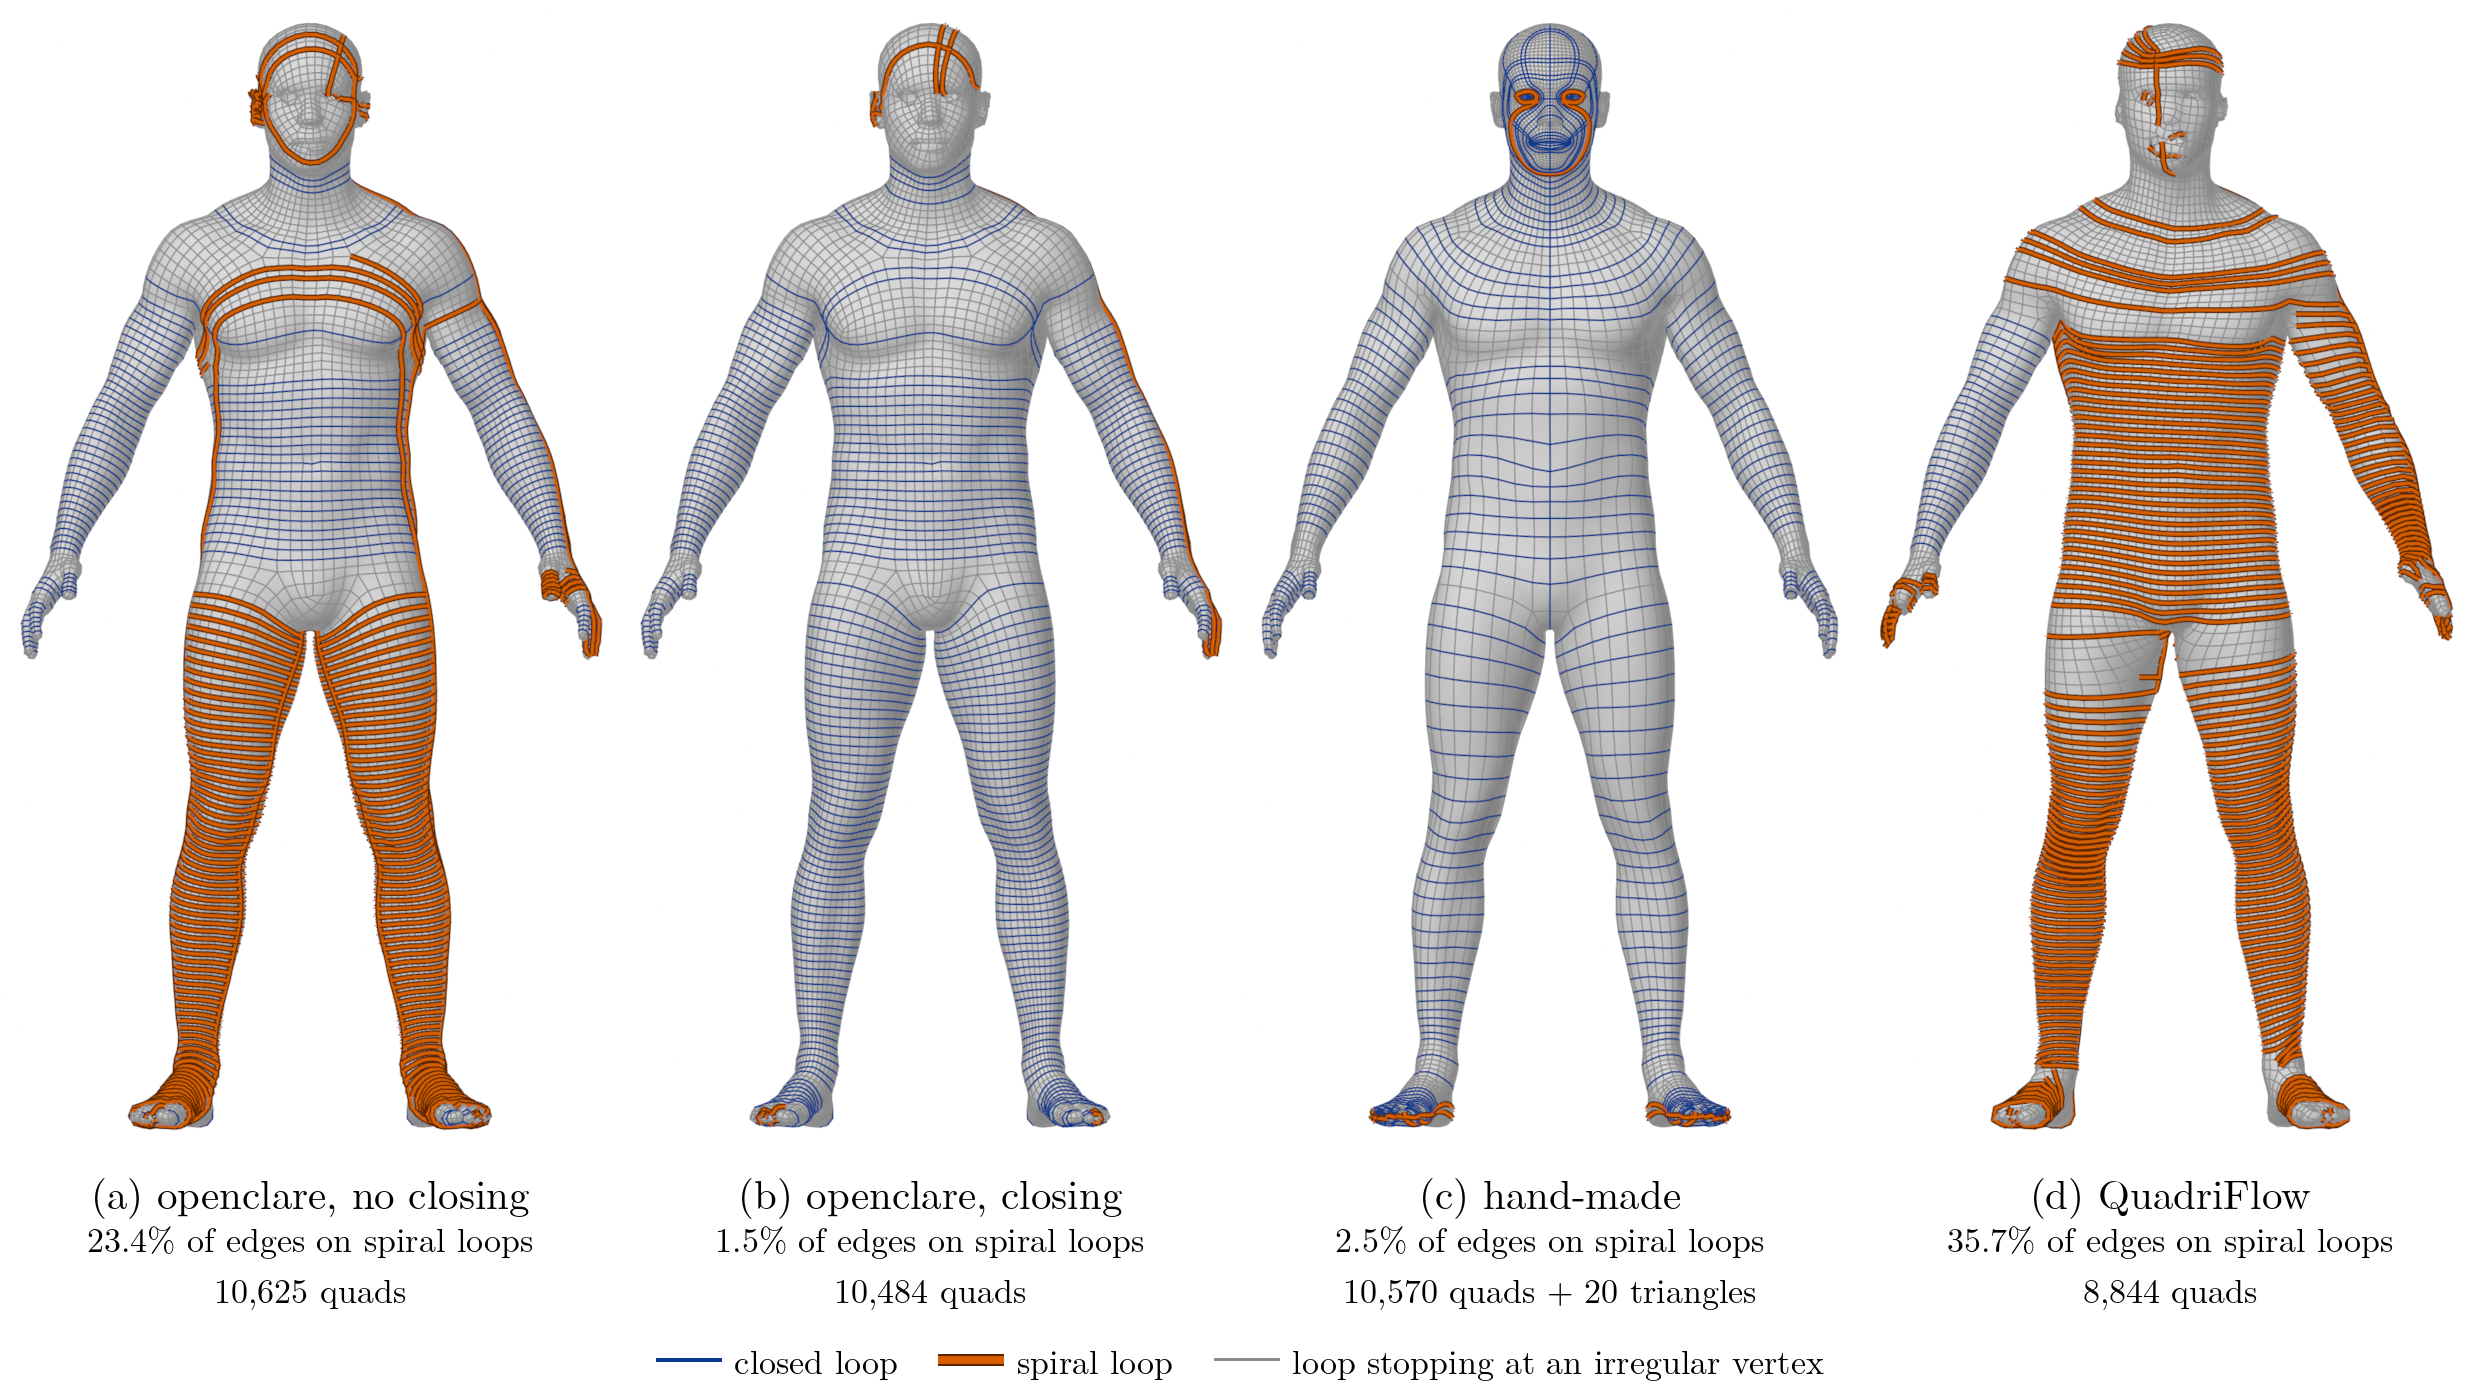
\includegraphics[width=\textwidth]{figures/male-overview.png}
\caption{The male body of the Essentials library, $10{,}590$ quads asked
for: (a)~openclare without closing, (b)~openclare with the closing of
Section~\ref{sec:closing}, (c)~the base mesh modelled by hand,
(d)~QuadriFlow run through Blender, on the source scaled by $100$ and scaled
back: Blender refuses the sculpt as it is, some of its edges being shorter
than its threshold of $10^{-4}$, and QuadriFlow does not depend on the scale.
Edge loops are coloured by their kind in
the measure of Section~\ref{sec:measure}: closed loops dark blue, spiral
loops vermillion (wider, with a dark rim), loops that stop at an irregular
vertex grey. Meshes (a) and (b) come from the engine of version 0.7.0, one
deterministic run each, the runs quoted in the text. Measured on the whole
meshes, they have $10{,}625$, $10{,}484$, $10{,}570$ (plus $20$ triangles)
and $8{,}844$ quads, $23.4\%$ ($21$ loops), $1.46\%$ ($11$), $2.55\%$ ($3$)
and $35.7\%$ ($43$) of their edges on spiral loops, which the panels round to
one decimal, and $17.2\%$, $36.5\%$, $31.6\%$ and $2.7\%$ on closed loops.
QuadriFlow's mesh has $3$ inverted faces and a Hausdorff distance of
$31$\textperthousand\ of the diagonal.}
\label{fig:overview}
\end{figure*}

\begin{figure*}[t]
\centering
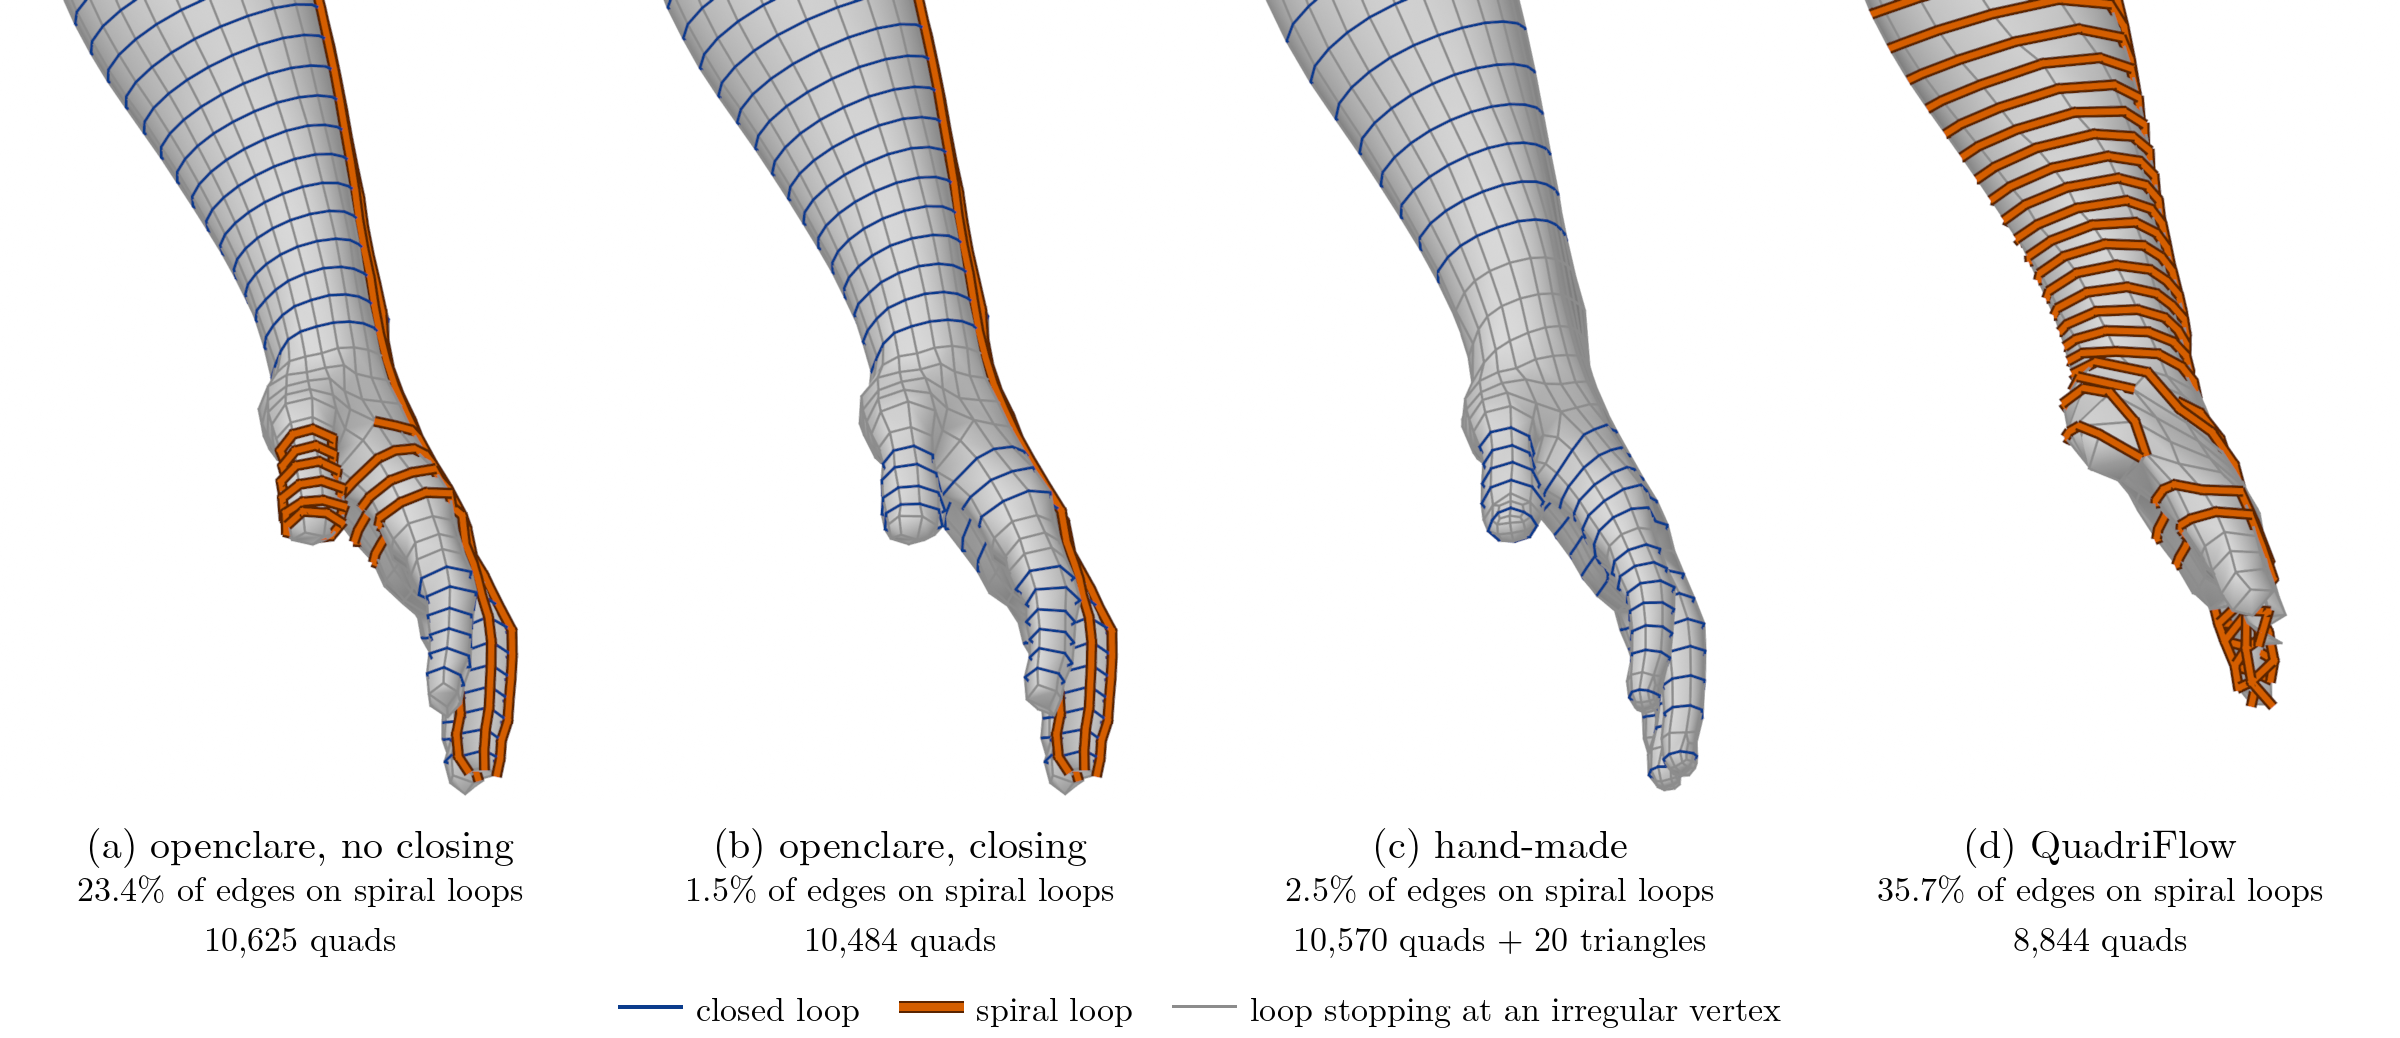
\includegraphics[width=\textwidth]{figures/male-wrist.png}\\[0.6em]
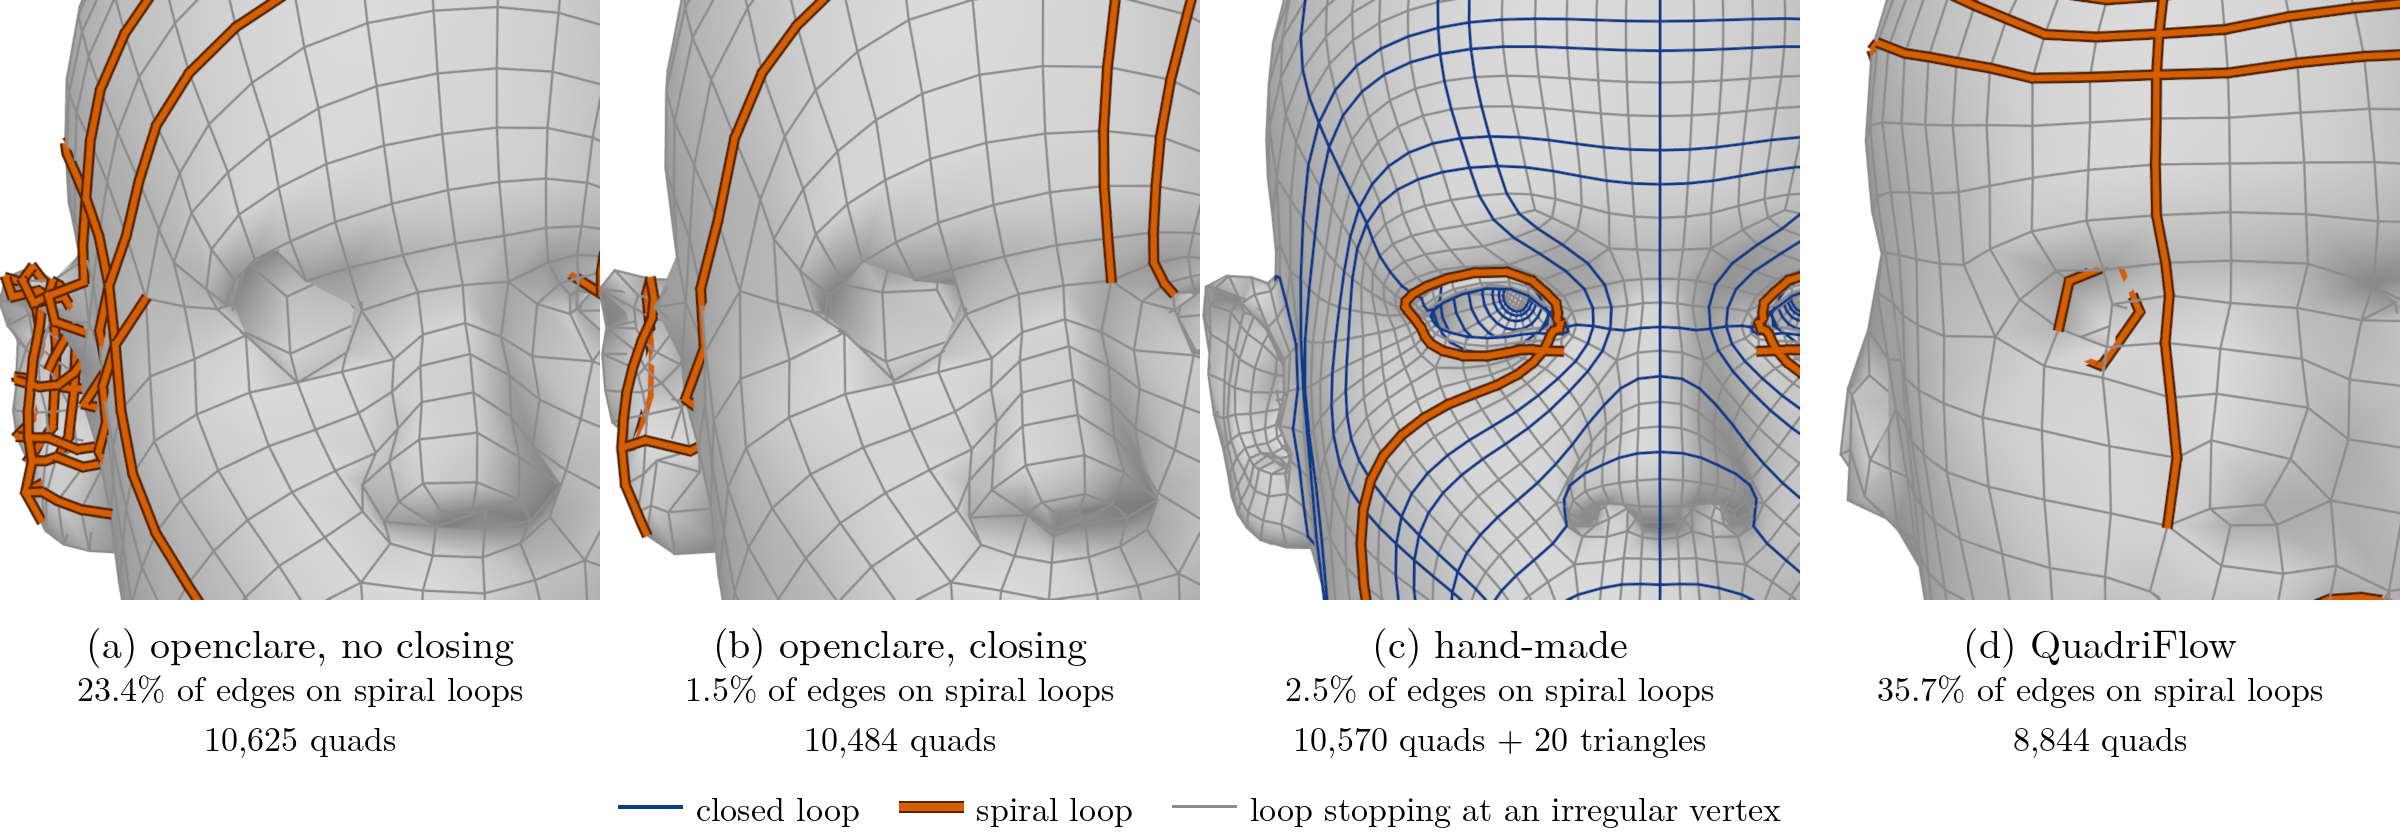
\includegraphics[width=\textwidth]{figures/male-eye.png}
\caption{Close-ups of the four meshes of Figure~\ref{fig:overview}, in the
same order and colours: the left wrist and hand (top; the body's left, on
the viewer's right in Figure~\ref{fig:overview}) and the right eye
(bottom). At the wrist, mesh~(b) has closed loops on the thumb and the back
of the hand where mesh~(a) has spiral ones, and a spiral loop along the outer
side of the forearm remains on both. At the eye, neither openclare mesh has
a spiral loop near the eye, both keep spiral loops on the forehead and at the
ear, and the loop round the eye of the hand-made mesh is itself counted as
spiral.}
\label{fig:closeups}
\end{figure*}

\section{An exact look at the closing system}\label{sec:exact}

How far is the heuristic of Section~\ref{sec:closing} from what the
constraints allow? An experiment option of the engine exports, for each way
of finding turns, the system it works on; we export it for the male body at
$10{,}590$ quads, from the engine as it runs. Its T-mesh has $1{,}342$ nodes
($1{,}068$ T-junctions, $254$ singular vertices, $131$ of valence three and
$123$ of valence five, and $20$ corners of folds), $2{,}146$ arcs and $806$
patches, hence $1{,}612$ balance equations, one per patch and direction. The
export gives the real lengths, every turn found with its shift (on all
$1{,}708$ turns, composing the crossing maps along the walk gives the
exported shift), and the lower bounds the integer search placed on arcs to
keep singularities apart ($36$ to $197$ arcs held at length one, depending on
the way). These bounds are the engine's choice of
\emph{which} arc of a chain between two singular vertices carries their
separation: validity asks a chain to keep a positive total length, not a
given arc. Every statement below is relative to them. We call
$P_{\mathrm{eng}}$ the balanced lengths that meet them; it is neither a
subset nor a superset of the valid quantizations, since it excludes valid
lengths that put the separation on another arc of the chain and allows
lengths that bring other arcs to zero. The ways are numbered as exported:
way $m + 2j + 4i$ starts from the shares $\{0.5\}$ ($m = 0$) or $\{0.2, 0.5,
0.8\}$ ($m = 1$), with the lean bound $0.05$ ($j = 0$) or $0.12$ ($j = 1$)
and the length bound $2$ ($i = 0$) or $6$ ($i = 1$) sides. Without the
other draws the engine keeps way~2 for this body ($1.65\%$ of spiral edges);
with them it keeps the lengths of another draw ($1.46\%$).

\paragraph{The conflict is real but local.}
All held turns can be closed together if the lengths are only asked to be
non-negative; with the bounds of separation, they cannot. By Farkas' lemma a
set of turns cannot be closed within the bounds exactly when some
combination of their shifts equals, modulo the balances, a non-negative
combination of arc lengths that charges an arc held open, and the companion
paper~\cite{gardent2026turns} reads these certificates on the singularities.
In seven ways (all but way~4) some held turn cannot even be closed on its
own. In five of them (0, 1, 2, 5 and 7) it is the same turn, of length
$6.76$, whose shift equals, modulo the balances, $-(\ell_{1892} +
\ell_{1908})$, where arc $1908$, less than $0.09$ quad edges long in the
parametrization, is held at length at least one; in ways 2, 3, 6 and 7 a
second turn, of length $4.72$, is held up in the same way by arc~$1006$ (both
certificates checked in exact rational arithmetic).
Whether $\ell_{1908} = 0$ would merge two singular vertices, that is whether
every valid quantization meets this bound, we did not check. Giving up the
least total amount of the bounds needed to close all held turns, a linear
program, shows that in way~0 the bound of arc $1908$ alone stands in the
way, in way~2 three bounds, that one among them, and in the other ways $6$
to $154$.

\paragraph{How many held turns can close.}
With every bound kept, the largest set of held turns that can be closed
together is found by a mixed-integer program with one binary per turn
(Table~\ref{tab:exact}). The projection of the engine keeps every held turn
closed: its active set asks the lengths to be non-negative only, which, as
above, lets all held turns close; the bounds of separation return in the
integer search. In whole numbers, the same mixed-integer program, with a
limit of fifteen minutes a way, proves its optimum in way~3 only ($90$
turns, as in real numbers); in the other ways it stops with $1$ to $88$
turns fewer than in real numbers.

\begin{table}[t]
\centering
\begin{tabular}{lrr}
\toprule
way & held & closable together \\
\midrule
0 & 58 & 57 \\
1 & 92 & 87 \\
2 & 64 & 61 \\
3 & 102 & 90 \\
4 & 125 & 120 \\
5 & 219 & 189 \\
6 & 131 & 123 \\
7 & 229 & 192 \\
\bottomrule
\end{tabular}
\caption{Male body at $10{,}590$ quads, real numbers, engine of version
0.7.0. ``Closable together'': the largest set of held turns closable with
every bound of separation kept; in way~7 the program stopped at its limit
of $300$ seconds, with a bound of $195$.}
\label{tab:exact}
\end{table}

\paragraph{The rounding ignores the shifts.}
Feeding the integer search of the engine better targets shows what survives
it (Table~\ref{tab:rounding}). The active-set projection, the engine's,
keeps every held turn closed in real numbers, yet after the integer search
$33\%$ to $74\%$ of them are shifted again ($170$ of $229$ in way~7); with a
least-squares projection whose negative lengths are clamped to zero, too,
about $40\%$ of the turns it closes are shifted after the integer search.
The integer search follows the targets but not the shifts. Aiming at the
lengths of the linear program, whose weighted $L^1$ objective puts the
changes on few arcs, the engine ranks first a candidate with $2.63\%$ of
spiral edges, yet outputs the mesh of the plain lengths: after meshing, the
candidates ranked before them were set aside.

\begin{table}[t]
\centering
\small
\begin{tabular}{lrrr}
\toprule
targets of the integer search & turns closed in reals & still shifted after & spiral edges (mesh) \\
\midrule
projection, clamped & 41--52 & 15--25 of them & 2.11\% \\
linear program, $L^1$ & 57--192 & 14--133 of them & 23.39\% \\
active set, floor 0 (the engine) & all held (58--229) & 19--170 of them & 1.46\% \\
active set, floor half the real length & 51--132 & 19--93 of them & 2.80\% \\
\bottomrule
\end{tabular}
\caption{Male body at $10{,}590$ quads, engine of version 0.7.0 with its
experiment options, one run each; ranges over the eight ways. The mesh keeps
the candidate with the fewest spirals, so its share is that of a single way
or draw; with the linear program it is the mesh of the plain lengths.}
\label{tab:rounding}
\end{table}

\paragraph{Whole lengths are not what is missing.}
The balances are the incidence matrix of a bidirected graph whose nodes are
the balance equations and whose edges are the arcs (each arc lies on a side
of each of the two patches it borders). When this graph is connected and has
a cycle that $\pm1$ values cannot balance, as on the body, the companion
paper shows that a set of free arcs parametrizes the lattice of whole
balanced lengths: here $2{,}146 - 1{,}612 = 534$ arcs can be given any whole
lengths and the others follow, so balances alone never obstruct whole
lengths. Closing exactly, in whole numbers, the turns found closable
together, HiGHS finds such lengths in $83$ to $228$ seconds in ways 0 to 3,
and none within ten minutes in ways 4 to 7. The solutions leave $1$, $5$,
$3$ and $12$ held turns shifted where the engine leaves $19$, $40$, $23$ and
$52$, and fewer of the turns not held as well ($3$ against $15$, $9$ against
$25$, $5$ against $18$, $11$ against $34$), at a weighted deviation from the
real lengths $2\%$ to $64\%$ higher. Yet three of the four spiral
\emph{more}, by the engine's count on the connectivity of their lengths:
$5.9\%$, $2.8\%$ and $7.8\%$ of their edges against $4.1\%$, $1.7\%$ and
$3.5\%$ for the engine's lengths in ways 0, 2 and 3; in way~1, $4.9\%$
against $9.1\%$. Only those of way~2 stay within the engine's window of
sizes; the others have $10{,}857$, $12{,}420$ and $11{,}011$ quads. Most of
the loops that spiral are not turns the sampled walks find.

Walking every strip of the mesh of way~2 instead
(Proposition~\ref{prop:complete}) finds $306$ ways round, each strip twice,
once in each direction; $236$ come back shifted. Selecting them by lean, as
the constraint rounds do, keeps $298$, of which $270$ ($135$ strips) can be
closed together in real numbers with every bound kept. Posed directly to
HiGHS, they gave no whole solution in $12{,}651$ seconds; given the $341$
arcs that every real solution sets to zero (each certified by a non-negative
combination of shifts, $216$ certificates over $36$ distinct sets of rings),
none was found in $2{,}596$ seconds either. No real lengths closing the
$270$ rings have a mean deviation from the targets below $1.304$, where the
engine allows $0.522$ ($0.2$ above the $0.322$ of its plain search). The
largest subset closable within a mean deviation of $0.4$, the number of
quads held to first order, found by a program stopped after $600$ seconds,
has $228$ rings (at most $267$) and closes at $0.395$ in real numbers. In
whole numbers, with the reformulation of Aardal, Hurkens and
Lenstra~\cite{aardal2000diophantine} on an LLL-reduced
basis~\cite{lenstra1982lll} of the lattice of closed quantizations, HiGHS,
stopped after $1{,}200$ seconds, finds whole lengths closing all $228$
within every bound at a mean deviation of $0.535$ and $10{,}653$ quads, and
proves that none does better than $0.518$. These lengths lie above the
engine's cap ($0.535$ against $0.522$), so the engine does not take them as
a candidate. Rounding costs between $0.123$ (proven) and $0.140$ (found) of
mean deviation above the real optimum.

\paragraph{The heuristic leaves most of the gap.}
The companion paper~\cite{gardent2026turns} computes the least number of
held turns that any lengths in $P_{\mathrm{eng}}$ leave shifted, a minimum
cover of the irreducible infeasible subsystems~\cite{parker1996iis}: exactly
$1$, $5$, $3$, $12$, $5$, $30$, $8$ and $37$ in ways 0 to 7, against $19$,
$40$, $23$, $52$, $61$, $154$, $72$ and $170$ left shifted by the engine.
With the engine's cap on the deviation and its window of sizes ($10{,}379$
to $10{,}801$ quads) added, at whole lengths, the least number is still
exactly one in way~0 and three in way~2: whole lengths closing every other
held turn exist at $10{,}730$ and $10{,}435$ quads, at mean deviations
$0.387$ and $0.506$. Of the $23$ turns of way~2 the engine leaves shifted,
the bounds of separation force three and the cap, the size and integrality
none; the heuristic accounts for $20$. Closing more turns, however, is not
what the measure of spirals sees: a local search over whole lengths within
the same cap and size closes $45$ more strips of the mesh of way~2 than the
engine does, but at its lengths, where the strips are other walks, $4.7\%$
of the edges spiral, against $1.7\%$ at the engine's lengths of way~2; it is
the choice of the turns to close, at the lengths where they are the strips
of the mesh, that decides how much the mesh spirals. Choosing the most turns to close
is NP-hard for bidirected balances with $0$--$1$ bounds, the algebraic form
of quantization~\cite{gardent2026turns}; whether the balances and turns of an
actual T-mesh stay hard is open.

\paragraph{Closing the most rings, end to end.}
We measured what an exact selection buys on the bench with the slow quality
mode of the engine (\texttt{--quality slow}), against the engine without its
other draws ($5.85\%$ of spiral edges over the $36$ runs), with three
($5.43\%$) and with its twelve ($4.92\%$). For the lengths the engine keeps,
a mixed-integer program closes as many of its strips leaning less than
$0.12$ as it can, weighted by their length round, within the balances, the
bounds of separation, the cap and the quad budget. A strip counts as closed
only where the corridor inequalities~\eqref{eq:corridor} hold for it, so
that it keeps its walk at the new lengths. The engine meshes the result, the
strips are walked again at the new lengths, and the program solved again,
three rounds; each round's lengths join the engine's candidates on the same
terms. The program is solved by HiGHS linked into the engine, each solve
stopped at a work limit (simplex iterations times arcs) that does not depend
on the load. Without the other draws, the slow mode lowers the mean to
$4.41\%$: lower on $9$ of the $36$ runs, never higher. Closed loops ($36.6\%$
against $35.4\%$ of the edges) and mean distance ($0.382$\textperthousand\
in both) barely move, and all $36$ meshes are valid. Against the twelve
other draws it is lower on average ($4.41\%$ against $4.92\%$) but not run
by run: higher on $9$ runs, lower on $5$. On the male body its three rounds
return the lengths they start from: $1.65\%$, as without it, against
$1.46\%$ for the engine with its draws. The gain does not need a solver that
finishes: $90$ of the $120$ solves stop at the work limit, and with a limit
of $5$ seconds per solve instead, $76$ of $100$ stop at it, $18$ of the $66$
rounds (against $12$) return the lengths they start from, and the mean is
$4.56\%$, on four processors where the other runs had eight.

\paragraph{Acting before quantization.}
Moving singular vertices in the parametrization, and rotating the field
cylinder by cylinder, were also tried, with prototypes of the engine that are
not part of it; neither lowered the share of spirals. The Burgers sum of the
companion paper~\cite{gardent2026turns} accounts for it: the shifts of two
parallel turns differ by the across component of the Burgers vector of the
singular vertices between them, which depends only on their developed
positions, so closing one turn by a local change of the map moves its shift
onto the turns beside it. The conflicts are better attacked in quantization.

\section{Limitations and open problems}\label{sec:limits}

The results come from one implementation and are preliminary. The spiral
share of a single model is chaotic, so only the means over three budgets are
robust; the other figures are single runs. The measure sees helices of pitch
up to four only. The exact look covers one body and holds relative to the
engine's bounds of separation, which are its choice of arcs and neither a
subset nor a superset of the valid quantizations. The machine was shared:
its load is recorded, not controlled, and the outcomes that depend on a
time limit depend on it.

Three problems remain open. \emph{An exact formulation}: minimizing the
deviation subject to the balances, the bounds and $\shift_\gamma(\ell) = 0$
for a set of turns is a minimum-deviation flow with linear side constraints;
how much of the exact machinery of~\cite{heistermann2023bimdf} carries over is
open, and the linear relaxation already closes $84\%$ to $98\%$ of the held
turns.
\emph{Closing in whole numbers}: whole lengths closing every ring asked for
are found through a reduced lattice basis, but in minutes, with the number
of quads held only to first order and $0.12$ to $0.14$ above the real optimum
in deviation, here above the engine's cap; can the integer search move within this lattice at the speed of
a flow solver? \emph{Which turns}, the central one on the evidence of
Section~\ref{sec:exact}: closing rings changes the lengths, the lengths
change the strips, and the strips of the new mesh are other walks. Is there a
finite set of turns whose closing implies that every loop of the quad mesh
closes? Can the loops of the quad mesh be read off the T-mesh and its lengths
directly, so that every one is accounted for? Which objective, short of all
loops, predicts the spirals the measure sees?

\section*{AI assistance}
This note and the software it describes were made by a human author working
with an AI system, which is not an author. The author chose the problem and
its aims (edge loops that close into rings and, as an artist, few singular
vertices and few spirals rather than perfectly square quads, quads only), set
the direction and the order of the work, decided which results to pursue and
which changes to merge, and judged the results through the measurements,
pictures and drafts presented to him. Claude Opus 5.5 (Anthropic), used
through Claude Code in October 2026 with several sub-agents in parallel,
wrote the changes to the engine and the experiment scripts, ran all the
experiments and exact computations, searched the literature, stated and
proved the propositions, and drafted the text. References were checked for
existence, and the note of each bibliography entry says how much of the work
was read. A work of which only the abstract, or a review, was read is cited only for what that abstract or review states. Weaker forms of Propositions~\ref{prop:linear}
and~\ref{prop:complete} are checked in Lean~4~\cite{demoura2021lean4} in the
companion paper, as the tag above each says; everything else here not checked by machine was written
with AI help and checked by AI agents rereading it and testing it on the
data, not by a human expert. The note has not been peer reviewed; the author,
who publishes it, is responsible for its content.

\bibliographystyle{plainnat}
\bibliography{refs}

\appendix

\section{Provenance of the figures}\label{app:provenance}

Every figure comes from the engine of version 0.7.0 (commit
\texttt{e13fadb}), built in release mode, and from the scripts of
\nolinkurl{docs/research/closing-loops/experiments/} (those of
Section~\ref{sec:exact} in its folder \nolinkurl{exact/}) and, for the
census, the conflicts and the least number of turns left shifted, which the
companion paper shares, of \nolinkurl{docs/research/turns-of-a-t-mesh/experiments/}.
Each script writes a summary, \texttt{results/}\textit{name}\texttt{.json}
beside it, with the engine's commit and build, the machine, its load and the
solver's version; its README gives the command of every table. The raw
output (meshes, exports, logs) is not in the repository.

\begin{center}
\small
\setlength{\tabcolsep}{4pt}
\begin{tabular}{@{}>{\raggedright\arraybackslash}p{5.6cm}>{\raggedright\arraybackslash}p{4.6cm}>{\raggedright\arraybackslash}p{4.4cm}@{}}
\toprule
figures & script & summary \\
\midrule
twelve models, three budgets (Section~\ref{sec:experiments})
  & \texttt{twelve\_models.py}, the protocol below
  & \texttt{twelve\_models.json} \\
Table~\ref{tab:dev}
  & \texttt{ablation.py}; its last line gave the $36$ meshes above byte for
  byte
  & \texttt{ablation.json} \\
against other remeshers
  & \texttt{against\_remeshers.py}, from \nolinkurl{bench/results/results.json}
  at \texttt{e13fadb}
  & \texttt{against\_remeshers.json} \\
male body, openclare and hand-made
  & \texttt{male\_body.py}
  & \texttt{male\_body.json} \\
Figures~\ref{fig:overview} and~\ref{fig:closeups}, their numbers
  & \texttt{figures/make\_figures.sh}, \texttt{figure\_numbers.py};
  QuadriFlow through Blender, on the source scaled by $100$ and scaled back
  & \texttt{figures.json} \\
Section~\ref{sec:exact}: the T-mesh, the conflicts, the least numbers left
shifted
  & \texttt{census.py}, \texttt{holonomy.py}, \texttt{conflicts.py},
  \texttt{forced.py} of the companion paper
  & their summaries of the same names \\
Section~\ref{sec:exact}: the other figures and Tables~\ref{tab:exact}
and~\ref{tab:rounding}
  & \texttt{exact/}: \texttt{relaxation.py}, \texttt{most\_closable.py},
  \texttt{rings.py}, \texttt{lattice\_rounding.py}, \texttt{local\_search.py},
  \texttt{remesh.py}
  & their summaries of the same names \\
closing the most rings, end to end
  & \texttt{exact/end\_to\_end.py}
  & \texttt{end\_to\_end.json}; the limit of $5$ seconds:
  \texttt{end\_to\_end-time-5.json} \\
\bottomrule
\end{tabular}
\end{center}

\paragraph{The protocol of the twelve models.} For each model $m$ (creature,
blob, suzanne, spot, pig, ogre, bob, jerry, blub, rock with the preset
\texttt{organic}; cage and part with \texttt{hard-surface}) and each budget
$Q \in \{2{,}970, 3{,}000, 3{,}030\}$: \texttt{openclare remesh}
\texttt{bench/out/}$m$\texttt{/source.obj} \textit{out.obj}
\texttt{--preset} $P$ \texttt{--quads} $Q$, then \texttt{openclare measure}
on the source and the output with \texttt{--target} $Q$ \texttt{--json}; the
figures are the means of \texttt{loop\_edges\_spiral},
\texttt{loop\_edges\_closed}, \texttt{loops\_spiral},
\texttt{mean\_distance} and \texttt{angle\_deviation\_mean} over the $36$
runs.

\paragraph{Reproducibility.} The method is implemented in openclare (Rust),
in the main branch of the repository; the bench is driven by
\texttt{bench/run.py}. The export of the T-mesh and the switches of
Table~\ref{tab:dev} are experiment options of the engine of version 0.7.0
(\texttt{ALGORITHM.md}, ``Experiment options''), and the slow quality mode
is its option \texttt{--quality slow}, so the scripts above make every
figure again on that engine; the figures that
depend on a time limit depend on the machine and its load as well. The
prototypes of ``Acting before quantization'' are not part of the engine and
are not scripted. This version of the note was built from commit
\texttt{\enginecommit}.

\end{document}
